
\documentclass[oneside,a4paper,14pt]{extreport}

% Font tiếng Việt
\usepackage[T5]{fontenc}
\usepackage[utf8]{inputenc}
\usepackage{amsmath}
\usepackage{amssymb}
\DeclareTextSymbolDefault{\DH}{T1}

% Tài liệu tham khảo

\usepackage[
	sorting=nty,
	backend=bibtex,
  style=numeric]{biblatex}

\usepackage[unicode]{hyperref} % Bookmark tiếng Việt
\addbibresource{References/references.bib}

\makeatletter
\def\blx@maxline{77}
\makeatother

% Chèn hình, các hình trong luận văn được để trong thư mục Images/
\usepackage{graphicx}
\graphicspath{ {Images/} }

% Chèn và định dạng mã nguồn
\usepackage{listings}
\usepackage{color}
\definecolor{codegreen}{rgb}{0,0.6,0}
\definecolor{codegray}{rgb}{0.5,0.5,0.5}
\definecolor{codepurple}{rgb}{0.58,0,0.82}
\definecolor{backcolour}{rgb}{0.95,0.95,0.92}
\lstdefinestyle{mystyle}{
    backgroundcolor=\color{backcolour},   
    commentstyle=\color{codegreen},
    keywordstyle=\color{magenta},
    numberstyle=\tiny\color{codegray},
    stringstyle=\color{codepurple},
    basicstyle=\footnotesize,
    breakatwhitespace=false,         
    breaklines=true,                 
    captionpos=b,                    
    keepspaces=true,                 
    numbers=left,                    
    numbersep=5pt,                  
    showspaces=false,                
    showstringspaces=false,
    showtabs=false,                  
    tabsize=2
}
\lstset{style=mystyle}


% Chèn và định dạng mã giả
\usepackage{amsmath}
\usepackage{algorithm}
\usepackage[noend]{algpseudocode}
\makeatletter
\def\BState{\State\hskip-\ALG@thistlm}
\makeatother

% Bảng biểu
\usepackage{multirow}
\usepackage{array}
\newcolumntype{L}[1]{>{\raggedright\let\newline\\\arraybackslash\hspace{0pt}}m{#1}}
\newcolumntype{C}[1]{>{\centering\let\newline\\\arraybackslash\hspace{0pt}}m{#1}}
\newcolumntype{R}[1]{>{\raggedleft\let\newline\\\arraybackslash\hspace{0pt}}m{#1}}

% Đổi tên mặc định
\renewcommand{\chaptername}{Chương}
\renewcommand{\figurename}{Hình}
\renewcommand{\tablename}{Bảng}
\renewcommand{\contentsname}{Mục lục}
\renewcommand{\listfigurename}{Danh sách hình}
\renewcommand{\listtablename}{Danh sách bảng}
\renewcommand{\appendixname}{Phụ lục}

% Định nghĩa
\newtheorem{definition}{Định nghĩa}
% Vẽ cây
\usepackage{tikz}
\usetikzlibrary{calc}
\usetikzlibrary{trees}

% Dãn dòng 1.5
\usepackage{setspace}
\onehalfspacing

% Thụt vào đầu dòng
\usepackage{indentfirst}

% Canh lề
\usepackage[
  top=30mm,
  bottom=25mm,
  left=30mm,
  right=20mm,
  includefoot]{geometry}
  
% Trang bìa
\usepackage{tikz}
\usetikzlibrary{calc}
\newcommand\HRule{\rule{\textwidth}{1pt}}
% ========================================================================================= %
% PACKAGE CUSTOMIZE
% pdf
\usepackage{pdfpages}

\usepackage[strings]{underscore}
\usepackage{url}

% Math
\usepackage{amsfonts}

\usepackage{stmaryrd}
\newcommand*\concat{\mathbin{\|}} % parallel

% Vẽ cây
\usetikzlibrary{trees}

% caption
\usepackage[justification=centering,font=small,labelfont=bf]{caption}
\captionsetup[figure]{font=small}
% % subfigure
\usepackage[font=small,labelfont=bf]{subcaption}
\usepackage{wrapfig}
% \usepackage[justification=centering,font=normalsize]{caption}

\renewcommand{\figureautorefname}{Hình}
% \renewcommand{\thesection}{\arabic{section}}
% \renewcommand\thesubsection{\alph{subsection}.}
\renewcommand{\thefigure}{\arabic{figure}}
\renewcommand{\theequation}{\arabic{equation}} % Change equation numbering style to consecutive numbers
\renewcommand{\equationautorefname}{Phương trình} % Change "Equation" to "Formula"
\usepackage{tocloft}
\usepackage{tabularx}
\usepackage{booktabs}

% Bảng thuật ngữ
\usepackage[acronym,nomain]{glossaries}

% Customize 
\usepackage[export]{adjustbox}
% ========================================================================================= %
% CHÚ Ý: Thông tin chung về KLTN - sinh viên điền vào đây để tự động update các trang khác  %
% ========================================================================================= %
\newcommand{\tenSV}{Hoàng~Minh~Thanh} % Dấu ~ là khoảng trắng không được tách (các chữ nối với nhau bằng dấu ~ sẽ nằm cùng 1 dòng
\newcommand{\mssv}{21C11029}
\newcommand{\tenKL}{XÂY DỰNG HỆ THỐNG SINH CỬ CHỈ TỪ ÂM THANH CHO TRỢ LÝ ẢO} % Chú ý dấu ~ trong tên khóa luận
\newcommand{\tenGVHD}{PSG. TS. Lý Quốc Ngọc}
\newcommand{\tenBM}{BM. Khoa~Học~Máy~Tính}

\begin{document}

\begin{titlepage}

\begin{center}
%ĐẠI HỌC QUỐC GIA THÀNH PHỐ HỒ CHÍ MINH\\
TRƯỜNG ĐẠI HỌC KHOA HỌC TỰ NHIÊN\\
\textbf{KHOA CÔNG NGHỆ THÔNG TIN}\\[2cm]

\begin{figure}[htp]
\centering

\includegraphics[width=8 cm]{images/logo-khtn.png}
% \caption{Hình ví dụ 1}
%\label{fig:vd1}
{\\[1cm]}
\end{figure}

{ \Large \bfseries \tenSV \\[1cm] } 

%Tên đề tài Khóa luận tốt nghiệp/Đồ án tốt nghiệp

%{ \Large \bfseries BÁO CÁO KHÓA LUẬN TỐT NGHIỆP \\
%OPENHUMAN.AI: HỆ THỐNG TỔNG HỢP CỬ CHỈ HỘI THOẠI DỰA TRÊN CẢM XÚC VÀ NGỮ NGHĨA \\[2cm]}
%{ \Large \bfseries BÁO CÁO KHÓA LUẬN TỐT NGHIỆP \\
%	DEEPGESTURE: MÔ HÌNH TỰ ĐỘNG GỠ RỐI CHO VIỆC HỌC CÁC ĐA TẠP CHUYỂN ĐỘNG CỬ CHỈ ĐỰA TRÊN GIỌNG NÓI \\[2cm]}
 
{ \Large \bfseries
	DEEPGESTURE: MÔ HÌNH TỰ ĐỘNG GỠ RỐI CHO VIỆC HỌC CÁC ĐA TẠP CHUYỂN ĐỘNG CỬ CHỈ ĐỰA TRÊN GIỌNG NÓI  \\[2cm]}
	
%	DeepGesture: Disentangled Autoencoders for Learning Speech-Driven Gesture Motion Manifolds


%Chọn trong các dòng sau
\large KHÓA LUẬN TỐT NGHIỆP THẠC SĨ\\
%\large ĐỒ ÁN TỐT NGHIỆP CỬ NHÂN\\
%\large THỰC TẬP TỐT NGHIỆP CỬ NHÂN\\
%Đưa vào dòng này nếu thuộc chương trình Chất lượng cao, hoặc lớp Cử nhân tài năng
% \large CHƯƠNG TRÌNH THẠC SĨ\\
% \large CHƯƠNG TRÌNH CHÍNH QUY\\
%\large CHƯƠNG TRÌNH CHẤT LƯỢNG CAO\\
%\large CHƯƠNG TRÌNH CỬ NHÂN TÀI NĂNG\\[2cm]


\begin{tikzpicture}[remember picture, overlay]
  \draw[line width = 2pt] ($(current page.north west) + (2cm,-2cm)$) rectangle ($(current page.south east) + (-1.5cm,2cm)$);
\end{tikzpicture}

\vfill
Tp. Hồ Chí Minh, tháng 12/2024

\end{center}

\pagebreak



\begin{center}

TRƯỜNG ĐẠI HỌC KHOA HỌC TỰ NHIÊN\\
\textbf{KHOA CÔNG NGHỆ THÔNG TIN}\\[2cm]


{\large \bfseries Hoàng Minh Thanh - 21C11029\\[2cm]}

%Tên đề tài Khóa luận tốt nghiệp/Đồ án tốt nghiệp

{ \Large \bfseries  BÁO CÁO KHÓA LUẬN TỐT NGHIỆP \\
	DEEPGESTURE: MÔ HÌNH TỰ ĐỘNG GỠ RỐI CHO VIỆC HỌC CÁC ĐA TẠP CHUYỂN ĐỘNG CỬ CHỈ ĐỰA TRÊN GIỌNG NÓI \\[2cm] } 
	
%	DeepGesture: Disentangled Autoencoders for Learning Speech-Driven Gesture Motion Manifolds

%Chọn trong các dòng sau
\large KHÓA LUẬN TỐT NGHIỆP THẠC SĨ \\

%\large ĐỒ ÁN TỐT NGHIỆP CỬ NHÂN\\
%Đưa vào dòng này nếu thuộc chương trình Chất lượng cao, hoặc lớp Cử nhân tài năng
% \large CHƯƠNG TRÌNH HOÀN CHỈNH\\[2cm]
%\large CHƯƠNG TRÌNH CHẤT LƯỢNG CAO\\[2cm]
%\large CHƯƠNG TRÌNH CỬ NHÂN TÀI NĂNG\\[2cm]

\textbf{GIÁO VIÊN HƯỚNG DẪN}\\
\tenGVHD\\
\tenBM\\

\begin{tikzpicture}[remember picture, overlay]
  \draw[line width = 2pt] ($(current page.north west) + (2cm,-2cm)$) rectangle ($(current page.south east) + (-1.5cm,2cm)$);
\end{tikzpicture}

\vfill
Tp. Hồ Chí Minh, tháng 09/2023

\end{center}

\end{titlepage}
% Sasu trang Title, các bạn chèn nhận xét gủa GVHD và GVPB. Nhận xét sẽ được giáo vụ phát sau buổi bảo vệ để các bạn đóng quyển.

\pagenumbering{roman} % Đánh số i, ii, iii, ...

\addcontentsline{toc}{chapter}{Lời cam đoan}
\chapter*{Lời cam đoan}
\label{reassurances}

Tôi xin cam đoan đây là công trình nghiên cứu của riêng chúng tôi. Các số liệu và kết quả nghiên cứu trong luận văn này là trung thực và không trùng lặp với các đề tài khác.

\addcontentsline{toc}{chapter}{Lời cảm ơn}
\chapter*{Lời cảm ơn}
\label{thanks}

%Tôi xin chân thành cảm ơn các thầy cô 

Chúng tôi xin chân thành cảm ơn thầy Lý Quốc Ngọc đã tận tình hướng dẫn, truyền đạt kiến thức và kinh nghiệm, và đưa ra các giải pháp cho chúng tôi trong suốt quá trình thực hiện đề tài luận văn tốt nghiệp này.

Xin gửi lời cảm ơn đến quý thầy cô Khoa Công Nghệ Thông Tin trường Đại Học Khoa Học Tự Nhiên - Đại Học Quốc Gia Thành Phố Hồ Chí Minh, những người đã truyền đạt kiến thức quý báu cho chúng tôi trong thời gian học tập vừa qua.

Đồng thời cảm ơn các nhà khoa học đã nghiên cứu về đề tài mà chúng tôi đã trích dẫn để có thể có những kiến thức hoàn thiện luận văn của chúng tôi.

Sau cùng chúng tôi xin gửi lời cảm ơn đến gia đình, bạn bè,.. những người luôn động viên, giúp đỡ chúng tôi trong quá trình làm luận văn. 

Một lần nữa, xin chân thành cảm ơn !

\addcontentsline{toc}{chapter}{Đề cương chi tiết}
%\includepdf[page={1,2,3,4}]{outline}

% Mục lục, danh sách hình, danh sách bảng
\addcontentsline{toc}{chapter}{Mục lục}
\tableofcontents
\listoffigures
\listoftables

\addcontentsline{toc}{chapter}{Tóm tắt}
\chapter*{Tóm tắt}
\label{abstract}

Việc xây dựng người kỹ thuật số (digital human) và các nhân vật trợ lý ảo siêu thực có khả năng tương tác giống như con người đã từ lâu trở thành mục tiêu nghiên cứu của các nhà khoa học máy tính. Sự tiến bộ trong đồ họa máy tính để mô phỏng người siêu thực, cùng với sự phát triển mạnh mẽ của phần cứng và thành công của các mô hình ngôn ngữ lớn, đã mở ra nhiều cơ hội mới. Tuy nhiên, thách thức lớn nhất hiện nay là sinh ra các biểu cảm khuôn mặt (facial expressions) và chuyển động của khung xương 3D  trước khi hiển thị trên màn hình cho người dùng. 
Sinh cử chỉ (gesture generation) không chỉ quan trọng trong việc phát triển các trợ lý ảo mà còn có ứng dụng trong game, robot và ngành công nghiệp điện ảnh. Để giải quyết vấn đề đồng bộ giữa âm thanh và cử chỉ, chúng tôi đề xuất phương pháp \textbf{DeepGesture}, dựa trên mô hình tự động gỡ rối với đầu vào là chuỗi cử chỉ khởi tạo và đoạn âm thanh tương ứng.


%Xây dựng người kỹ thuật số (digital human) hay các nhân vật trợ lý ảo siêu thật có thể tương tác như một con người là mục tiêu nghiên cứu từ lâu của các nhà khoa học máy tính. Với sự phát triển của đồ họa máy tính trong việc mô phỏng người siêu thật cũng như sự phát triển mạnh mẽ của phần cứng máy tính và thành công của các mô hình ngôn ngữ lớn gần đây.
%Thì nút thắt cổ chai duy nhất hiện nay là việc sinh ra các biểu cảm khuôn mặt (facial expression), cũng như các khung xương (joins) 3D trước khi kết xuất (render) để hiển thị lên màn hình cho người dùng.
%Sinh cử chỉ (gesture generation) không chỉ được sử dụng để xây dựng người trợ lý ảo mà còn được sử dụng trong game, robot cũng như trong công nghiệp điện ảnh.
%Để giải quyết vấn đề đồng bộ giữa âm thanh và cử chỉ, chúng tôi đề xuất phương pháp \textbf{OHGesture} dựa trên mô hình diffusion với đầu vào là chuỗi cử chỉ khởi tạo, và đoạn âm thanh tương ứng.	
%Đóng góp của tôi là sử dụng văn bản và cảm xúc, sử dụng cơ chế cross-attention và self-attention trong quá trình diffuse để sinh cử mượt mà và chân thực.
%
%Thực nghiệm chứng minh phương pháp của chúng tôi có thể giúp chúng tôi tạo ra cử chỉ theo nhiều cảm xúc khác nhau và đạt kết quả tốt hơn khi áp dụng cross-attention.

% Ngoài ra mô hình OHGesture cũng sinh được các cử chỉ với đa dạng cảm xúc khác nhau như vui vẻ, buồn bã, người già.

% OHGesture sẽ biểu diễn các dự liệu đầu vào thành các vùng trong không gian với mỗi vùng một đại diện tương ứng. Sau đó sắp xếp lại vị trí đại diện của mỗi vùng dựa trên khoảng cách với cử chỉ khởi tạo để tạo ra các chuỗi cử chỉ ứng viên.

% Cử chỉ sinh ra do người nói có tính tuần hoàn, dựa vào phương pháp mã hóa tuần hoàn (Periodic Autoencoders \cite{starke2022deepphase} ), mô hình sẽ trích xuất được các pha (phrase) của cử chỉ, từ đó giúp mô hình chọn được cử chỉ có pha phù hợp với ngữ nghĩa hoặc nhịp điệu của lời nói.
% Đóng góp của chính của chúng tôi là 

Mã nguồn của chúng tôi được công khai ở

\href{https://github.com/DeepGesture/DeepGesture}{DeepGesture/DeepGesture}

\clearpage

\pagenumbering{arabic} % Đánh số 1, 2, 3, ...

% Các chương nội dung
% Giới thiệu
% \usepackage[utf8]{inputenc}
% \usepackage[T1]{fontenc}%❖ Là chương mở rộng của tóm tắt
%❖ Nội dung bao gồm
%o Ngữ cảnh, vấn đề cần giải quyết là gì?
%o Vì sao vấn đề/bài toán quan trọng và thú vị?
%o Bài toán có gì khó? Vì sao cần phải giải quyết?
%o Những giải pháp (nghiên cứu, ứng dụng) đã giải quyết bài toán này?
%o Những giải pháp này có hạn chế, thiếu sót gì?
%o Giải pháp của bạn là gì? Kết quả thế nào?
%o Đóng góp của nghiên cứu/ứng dụng của bạn? 
%❖ Độ dài từ 3 đến 8 trang
%❖ Có thể chia ra các mục
%o Đặt vấn đề (Problem)
%o Mục tiêu (Objectives)
%o Giải pháp/Cách tiếp cận (An Approach)
%o Đóng góp (Contributions)
%o Bố cục (Outline)
%❖ Lưu ý, nội dung các chương sau phải khớp với mục tiêu, giải pháp, đóng góp ở chương này
\chapter{Giới thiệu}
\label{Chapter1}

\section{Bối cảnh chung}

\begin{figure}[h!]
  \centering
  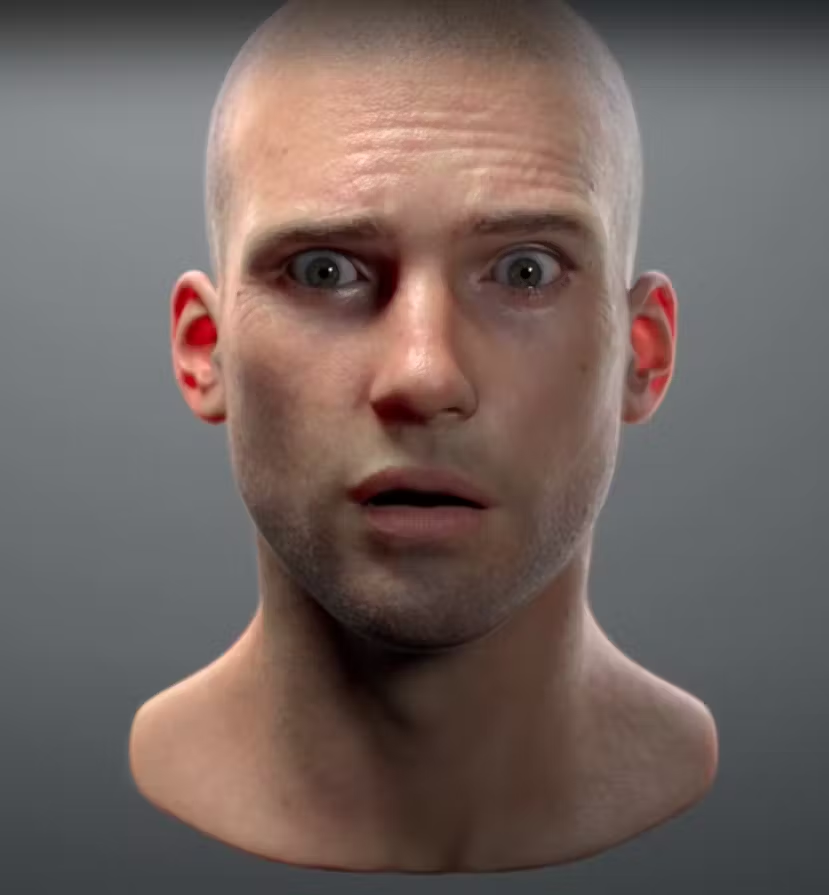
\includegraphics[width=0.5\linewidth]{images/cgi.png}
  \caption{Công nghệ CGI với người kỹ thuật số siêu thật}
  \label{fig:cgi}
\end{figure}

Mỗi ngày, trên thế giới có hàng tỷ người nhìn vào màn hình RGB, kết quả hiển thị trên màn hình là đầu ra của mọi hệ thống phần mềm, nên việc hiển thị từng pixel trên màn hình và cách để mô phỏng lại hình ảnh trên một cách chân thực nhất được các nhà khoa học về đồ họa máy tính (Computer Graphic) nghiên cứu từ những năm 1960s và đặc biệt là việc mô phỏng lại con người \autoref{fig:cgi}. 

Ngày nay, công nghệ đồ họa máy tính đã hoàn toàn có thể mô phỏng nhiều vật giống đến mức siêu thực (realistic) các vật phức tạp như nước, đường xá, bánh mỳ,...  và thậm chí là cả cơ thể và khuôn mặt con người với độ chi tiết đến từng lông tơ, nốt mụn và vân mắt. 
Vào năm 2015, bằng kỹ thuật quyét 3 chiều ghi lại toàn bộ các góc của khuôn mặt, sự phản chiếu ánh sáng, trong công trình \cite{metallo2015scanning}
nhà khoa học đồ họa máy tính đã có thể tái tạo toàn bộ khuôn mặt của tổng thống Obama trên máy tính với độ chính xác cao và gần như không thể phân biệt \autoref{fig:obamascan}.

\begin{figure}
    \centering
    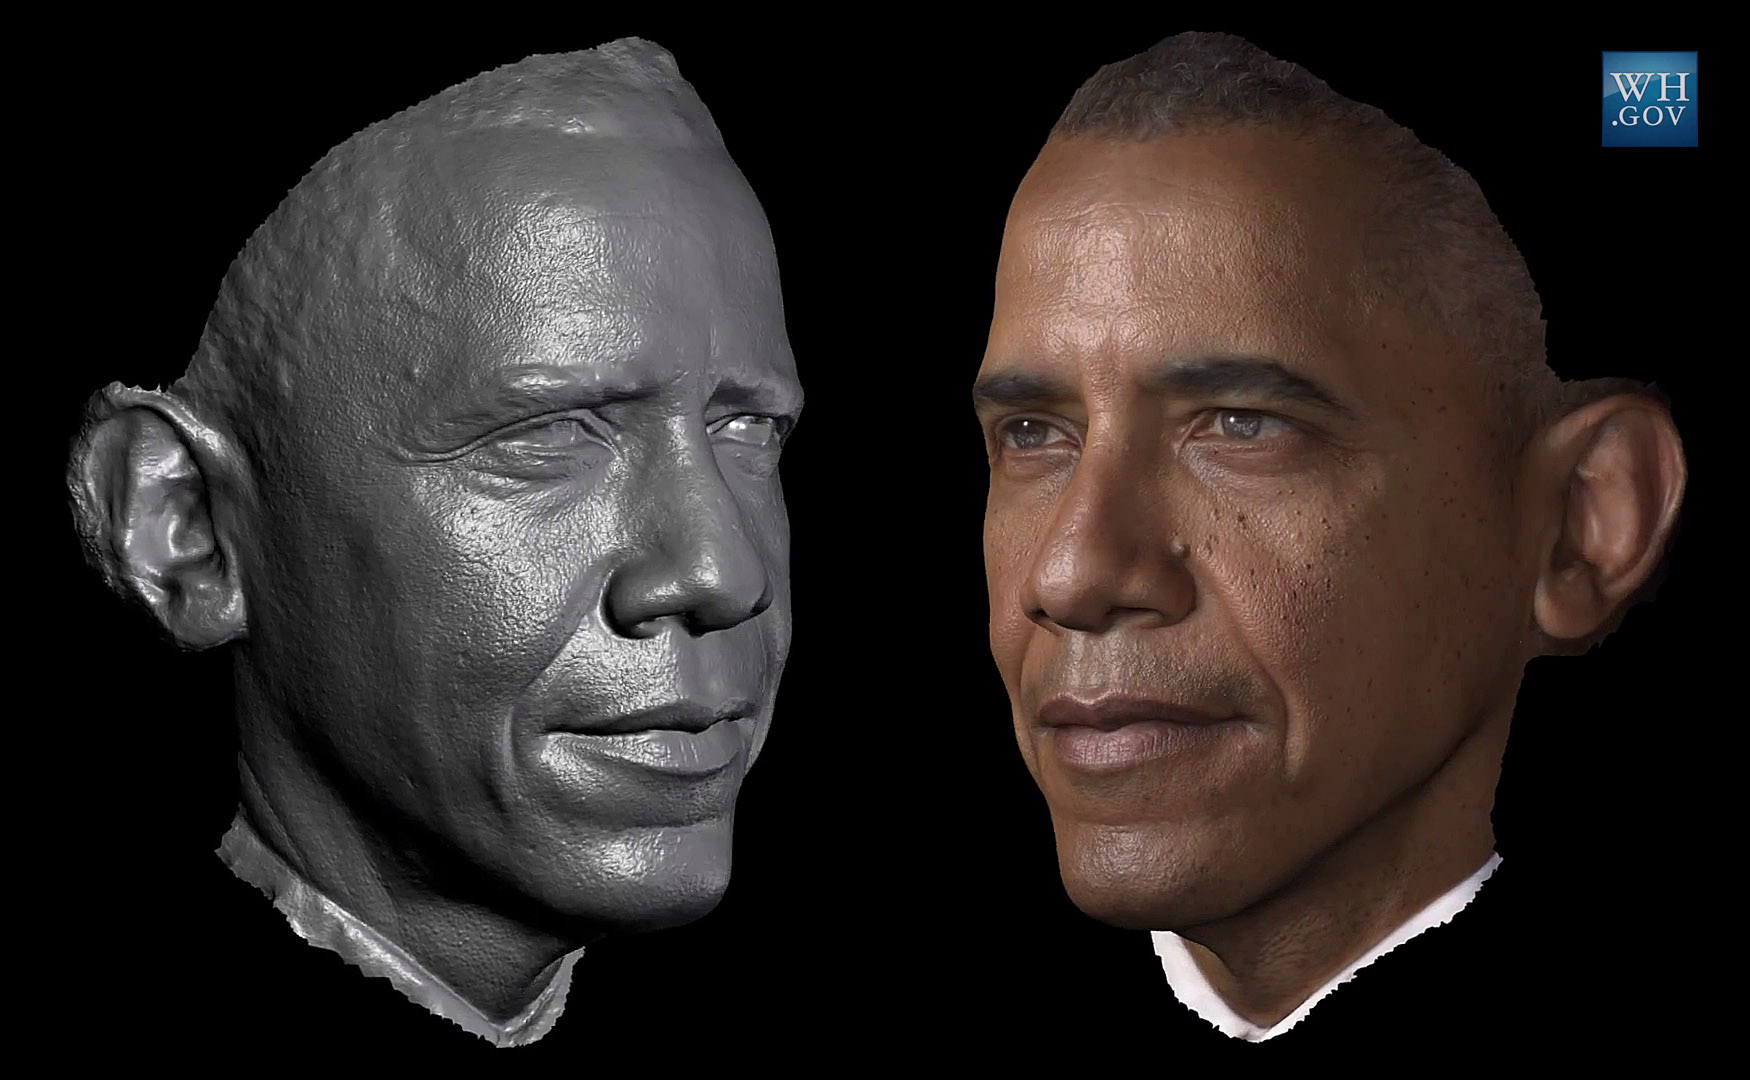
\includegraphics[width=\linewidth]{images/obama_scan.jpg}
    \caption{Minh họa công trình tái tạo khuôn mặt tổng thống Obama}
    \label{fig:obamascan}
\end{figure}

Trí tuệ nhân tạo thể hiện kết quả vượt bậc những năm gần đây không chỉ trong nghiên cứu mà con trong ứng dụng thực tế, tiêu biểu như ứng dụng ChatGPT, Midjouney và sự phát triển cả theo chiều dọc và chiều ngang trong việc ứng dụng trí tuệ nhân tạo với nhiều lĩnh vực khác nhau. Mặc dù đồ họa máy tính đã có thể xây dựng khuôn mặt người siêu thật, việc sinh cử chỉ lại phụ thuộc vào việc Chụp chuyển động (Motion Capture) từ các cảm biến và gặp rất nhiều khó khăn khi xây dựng một hệ thống trí tuệ nhân tạo để học từ dữ liệu.

Các hệ thống trí tuệ nhân tạo hiện nay đã có thể tạo văn bản và âm thanh tiệm cận như con người, nhưng một trong những trở ngại lớn nhất để xây dựng con người kỹ thuật số hiện nay chính là việc sinh cử chỉ. Chính vì vậy mà mục tiêu của luận văn là xây dựng một hệ thống sinh cử chỉ hội thoại dựa trên cảm xúc và ngữ nghĩa với dữ liệu đầu vào gồm cả văn bản và giọng nói.

\section{Động lực nghiên cứu}

% Ý nghĩa khoa học và ứng dụng của đề tài
% Vai trò của việc sinh cử chỉ
Tổng hợp cử chỉ hội thoại giúp ích cho rất nhiều lĩnh vực như hoạt ảnh, dựng phim, trò chơi điện tử, giáo dục và những ứng dụng thực tại ảo. Việc tổng hợp cử chỉ chuyển động được thực hiện theo cách truyền thống là thuê các diễn viên sử dụng các tracker và bố trí các hệ thống cảm biến xung quanh thu nhận chuyển động để đạt được độ chính xác nhân thực nhất. Tuy nhiên, các chuyển động thu được sau đó chỉ được phát lại và không có sự biến chuyển giữa các hành động hay chuyển động, chính vì vậy, việc áp dụng trí tuệ nhân tạo để có thể học các chuyển động từ dữ liệu thu nhận và sau đó có thể sinh ra dữ liệu mới sẽ là một cuộc cách mạng trong ngành công nghiệp Motion Capture.

Vào năm 2011, một nhóm tác giả \cite{bergmann2011relation} đã chứng minh rằng có sự liên hệ giữa giọng nói và cử chỉ con người, đây chính là tiền đề để cho thấy chúng ta có thể dùng dữ liệu âm thanh để có thể dùng để học và biểu diễn được cử chỉ con người.
Với sự thành công của các mô hình ngôn ngữ tự nhiên trong việc xử lý ngôn ngữ văn bản, với sự chính xác siêu thật trong việc mô phỏng gương mặt con người trong lĩnh vực Đồ họa máy tính và với sự chính xác và dễ dàng từ việc tổng hợp giọng nói con người hiện nay. Thì việc ứng dụng trí tuệ nhân tạo để sinh cử chỉ con người là một trong những điểm nghẽn cổ chai duy nhất trong việc phát triển một trợ lý ảo để trao đổi và tương tác với con người.

\section{Phát biểu bài toán}

Mục tiêu của việc sinh cử chỉ (gesture generation) bằng phương pháp học máy là tạo ra các cử chỉ tự nhiên (naturalness), chân thật (realistic) như con người và đồng thời phù hợp với ngữ cảnh.
%Sinh cử chỉ (gesture generation) là bài toán dựa vào những dữ liệu trước đó bao gồm văn bản và âm thanh, cử chỉ khởi tạo để nội suy ra chuỗi cử chỉ tiếp theo.
Sinh cử chỉ là bài toán hồi quy (regression), với đầu vào là một chuỗi cử chỉ cho trước và kết quả đầu ra là chuỗi cử chỉ tiếp tục với cử chỉ trước đó.

Mỗi khung hình chuyển động của một nhân vật hay khung xương (skeleton) bao gồm dữ liệu về toạ độ vị trí và vận tốc theo thời gian.
Ở đây dữ liệu của chúng tôi của một khung xương với mỗi khung hình (frame) bao gồm:

\begin{equation} \label{eq:gesturevector}
\mathbf{g} = \Big[ \mathbf{p}_{\text{root}},  \mathbf{r}_{\text{root}},
\mathbf{ p }'_{\text{root}},  \mathbf{r}'_{\text{root}},
\mathbf{p}_{\text{joins}},  \mathbf{r}_{\text{joins}},
\mathbf{p}'_{\text{joins}},  \mathbf{r}'_{\text{joins}},
\mathbf{d}_{\text{gaze}}
\Big]
\end{equation}

Trong  đó với mỗi $\mathbf{g} \in \mathbb{R}^{1141}$ bao gồm:
\begin{itemize}
	\item $\mathbf{p}_{\text{root}} \in \mathbb{R}^3$: Toạ độ của điểm gốc
	\item $\mathbf{r}_{\text{root}} \in \mathbb{R}^4$: Góc quay của điểm gốc
	\item $\mathbf{p}'_{\text{root}} \in \mathbb{R}^3$: Vận tốc thay đổi của toạ độ gốc
	\item $\mathbf{r}'_{\text{root}} \in \mathbb{R}^3$: Vận tốc thay đổi của góc quay gốc
	
	\item $\mathbf{p}_{\text{joins}} \in \mathbb{R}^{3 n_{\text{join} }}$: Toạ độ của các khung xương
	\item $\mathbf{r}_{\text{joins}} \in \mathbb{R}^{3 n_{\text{join} }}$: Góc quay của các khung xương
	\item $\mathbf{p}'_{\text{joins}} \in \mathbb{R}^{3n_{\text{join} }}$: Vận tốc thay đổi của toạ độ các khung xương
	\item $\mathbf{r}'_{\text{joins}} \in \mathbb{R}^{3n_{\text{join} }}$: Vận tốc thay đổi của góc quay các khung xương
	
	\item $\mathbf{d}_{\text{gaze}} \in \mathbb{R}^3$: Là hướng nhìn
\end{itemize}

%\begin{figure}
%	\centering
%	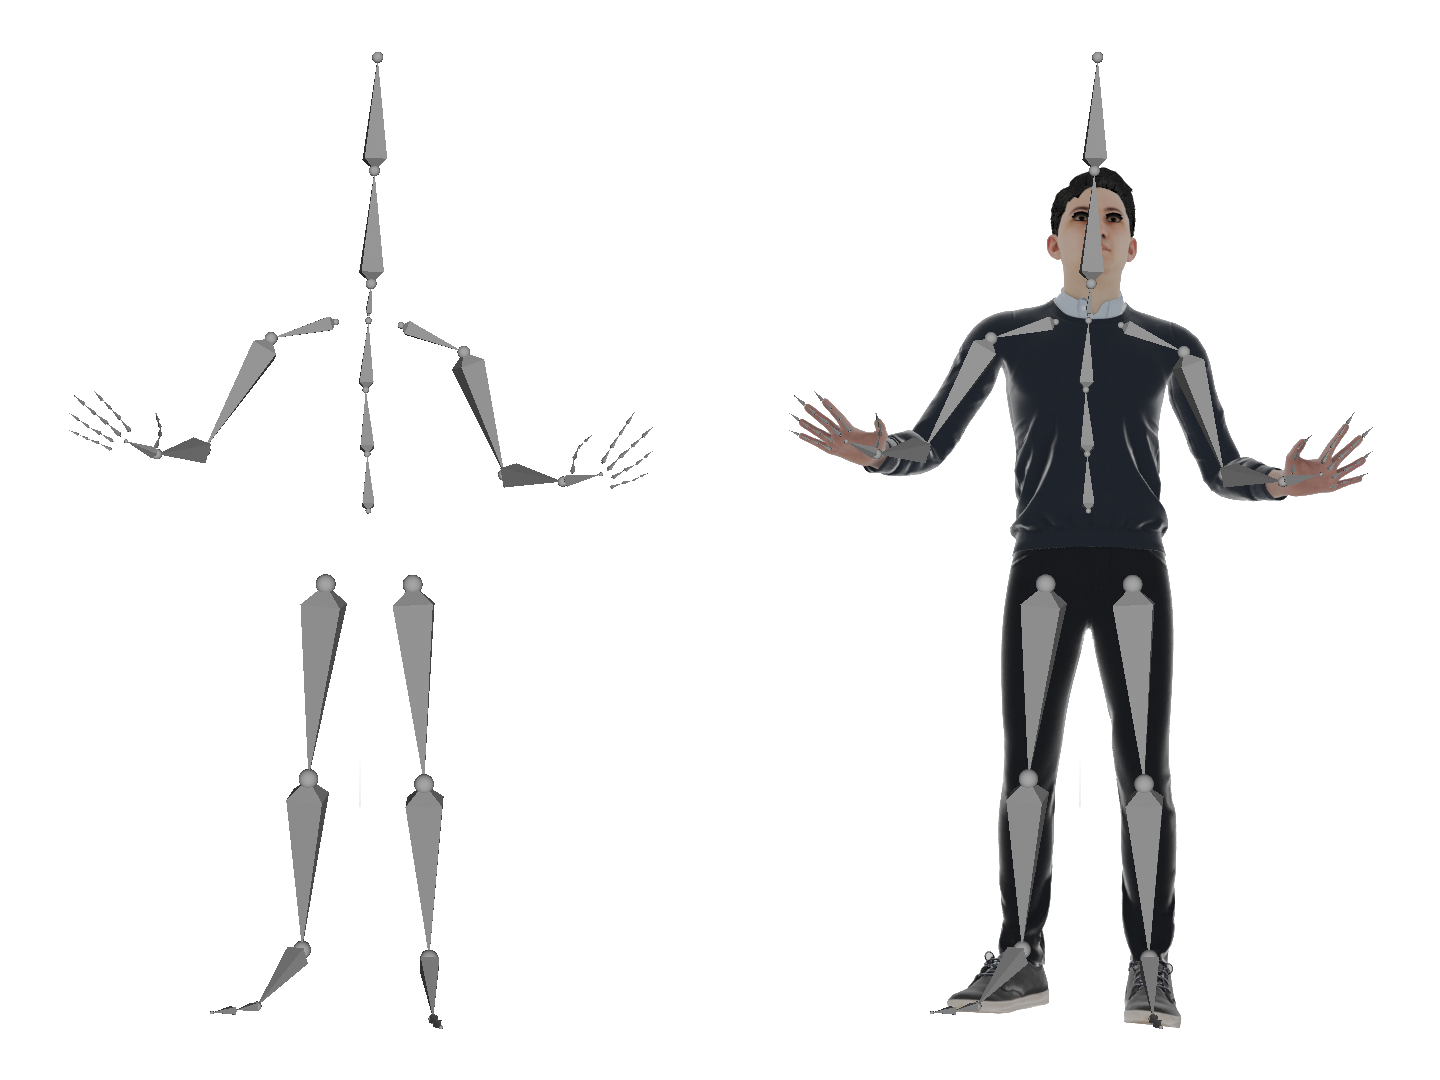
\includegraphics[width=0.8\linewidth]{images/skeleton_sample.png}
%	\caption{Minh họa một cử chỉ và mô hình nhân vật}
%	\label{fig:software}
%\end{figure}
\begin{figure}
	\centering
	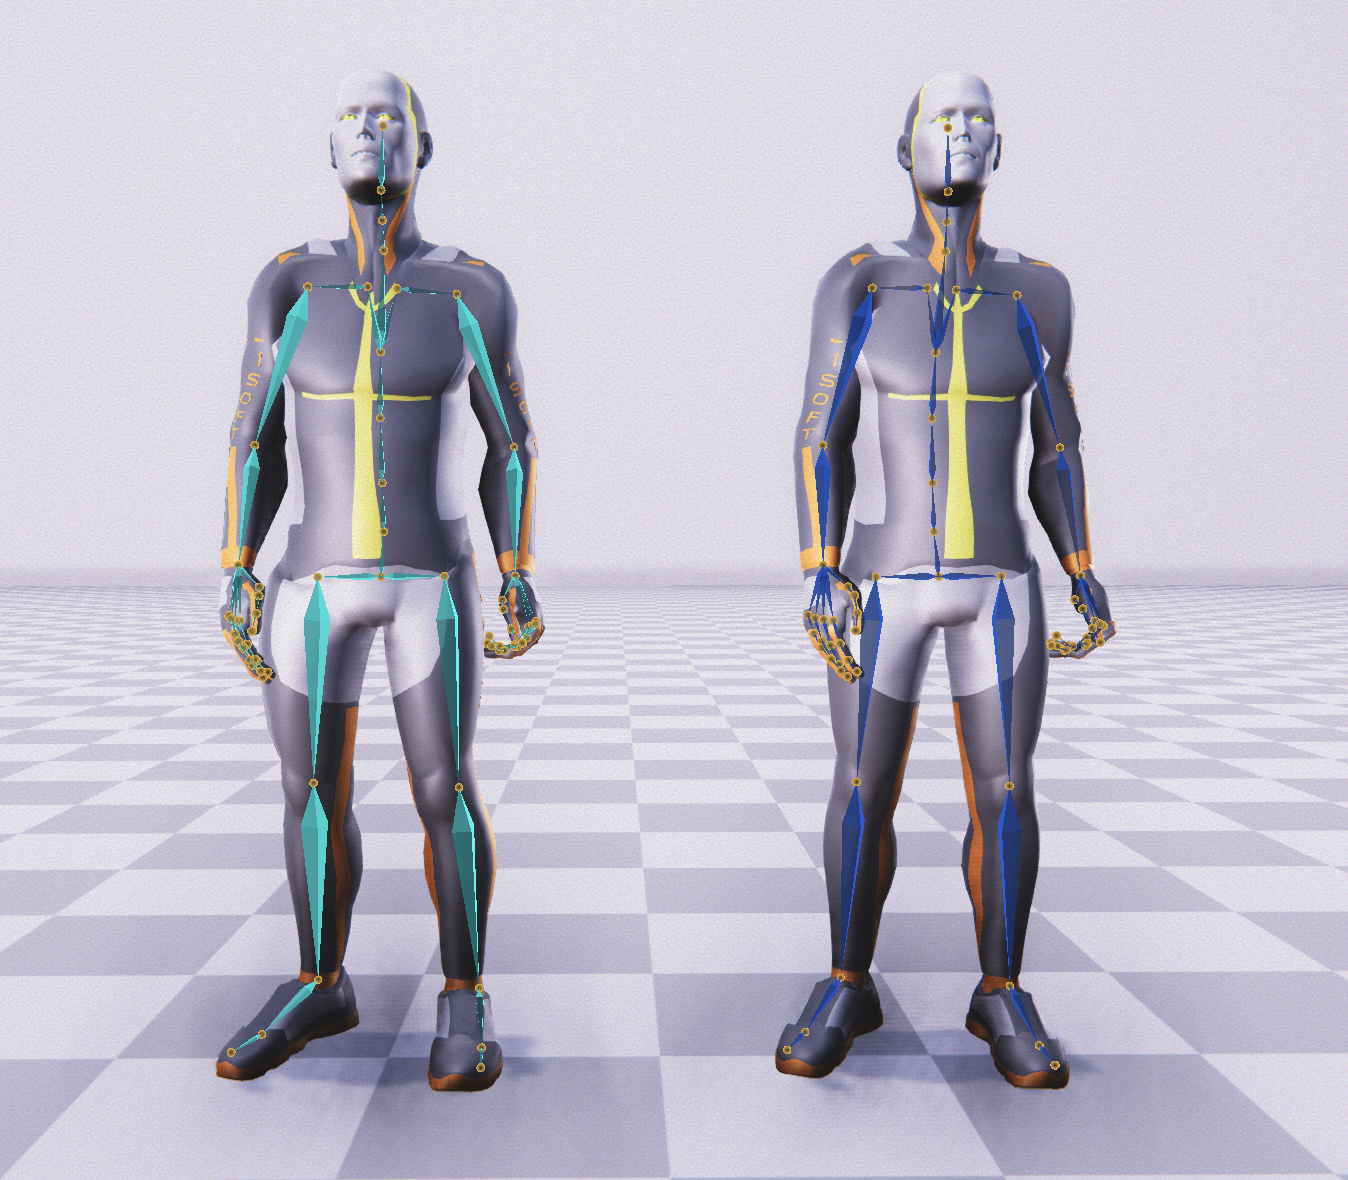
\includegraphics[height=10cm]{images/AnimationSample.png}
	\caption{Minh hoạ khung xương của nhân vật.}
	\label{fig:AnimationSample}
\end{figure}

Tổng cộng có $75$ khớp (joins) hay $n_{\text{join}} = 75$, với mỗi khung hình (frame) ta sẽ có một vector gồm 1141 chiều.
Tập dữ liệu là tập nhiều chuỗi cử chỉ với độ dài tuỳ ý, từ mỗi cử chỉ độ dài tuỳ tý ta sẽ cắt thành các đoạn $8 + N$ khung hình, $g \in \mathbb{R}^{(8+N) \times 1141}$ , trong đó cử chỉ $g \in \mathbb{R}^{8 \times 1141}$ đầu tiên là cử chỉ khởi tạo (seed gesture), $g \in \mathbb{R}^{N \times 1141}$ cử chỉ tiếp theo cho việc dự đoán.

Dữ liệu âm thanh $\mathbf{a}_{\text{raw}} \in \mathbb{R}^{ \text{wave\_size } }$  là một chuỗi waveform có độ dài tương ứng với cử chỉ được đọc với sample rate là 16000. Chuỗi waveform sẽ được cắt thành các đoạn chồng nhau, áp dụng Hamming windows, và áp dụng thuật toán fast fourier transform để biến đổi chuỗi âm thanh thành các hệ số thể hiện cường độ của các tần số trong chuỗi âm thanh, các hệ số này được làm tròn thành các đoạn tần số (frequency bins), các đoạn hệ số này được chuẩn hoá theo hệ cơ số log để tương ứng với cảm nhận của tai người để có được đặc trưng MFCC $\mathbf{a} \in \mathbb{R}^{\text{size} \times \mathcal{C}}$ trong đó $\mathcal{C}=13$ là số frequency bins. 


% \begin{figure}
%     \centering
%     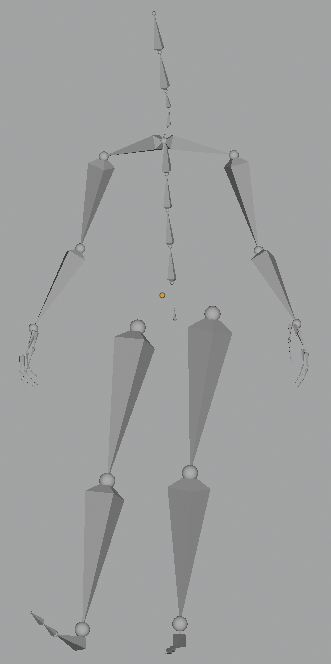
\includegraphics[width=3cm]{images/gesture_sample.png}
%     \caption{Minh họa cử chỉ}
%     \label{fig:gesture_sample}
% \end{figure}

\section{Các khó khăn cần giải quyết}

Có rất nhiều khó khăn trong việc xây dựng một mô hình có thể học được các đăng trưng cử chỉ hội thoại như con người theo thời gian thực:

Thứ nhất, \textit{dữ liệu không đủ nhiều và chất lượng}, chi phí để tạo ra một bộ dữ liệu trong ngành công nghiệp Motion Capture có chất lượng và quy mô lớn để ứng dụng vào trong thực tế là rất lớn.

Thứ hai, \textit{sự thiếu đồng nhất của về ngữ cảnh của các loại dữ liệu}, các bộ dữ liệu về văn bản thường rất nhiều hơn so với giọng nói và cũng không thể biết được văn bản đó được tạo bởi người nào, sự đồng bộ giữa giọng nói và cảm xúc lúc nói cũng thiếu trong việc tạo tập dữ liệu. Ngoài ra, các dữ liệu văn bản lại được nói bởi rất nhiều người khác nhau và ở nhiều nội dung và chủ đề khác nhau.
 
Thứ ba, \textit{sự phân bố không cân xứng về  dữ liệu giữa các loại đăng trưng cần học}. Các dữ liệu dùng cho nghiên cứu cử chỉ hiện nay thường tập trung vào ngôn ngữ Tiếng Anh, các cử chỉ có sự phân bố không cân xứng giữa khi nói, khi hỏi, khi im lặng.

Thứ tư, \textit{chi phí tính toán với nhiều loại dữ liệu của mô hình rất lớn}. Với đầu vào của mô hình gồm rất nhiều loại dữ liệu khác nhau như văn bản, tiếng nói và điểm 3D, nên cần rất nhiều lớp encode cho từng loại dữ liệu cũng là rào cản không nhỏ bởi chi phí tính toán khi huấn luyện và khi suy luận. Nếu giảm thông tin dữ liệu đầu vào cũng sẽ giảm kết quả suy luận của mô hình khi sinh cử chỉ.

Cuối cùng, \textit{các bước xử lý phải yêu cầu tuần tự}, cách hiệu quả nhất để con người tương tác với máy tính là thông qua giọng nói và nhập từ bàn phím, tuy nhiên việc xử lý được văn bản và giọng nói để làm đầu vào cho mô hình phải thực hiện tuần tự, độ trễ để có thể suy luận trong sản phẩm thực tế cũng là một vấn đề bởi người dùng không thể đợi lâu để nhận được kết quả cử chỉ và từ cử chỉ đó biểu diễn lên máy tính bằng kỹ thuật đồ họa máy tính.


\section{Đóng góp của chúng tôi}

\begin{itemize}
\item Chúng tôi mở rộng mô hình diffusion với thông tin thời gian cho việc sinh cử chỉ kèm theo lời nói dựa trên âm thanh. Nhờ mô hình diffusion, chúng tôi có thể kiểm soát một cách linh hoạt cử chỉ được sinh ra, ví dụ: chỉnh sửa phong cách của cử chỉ, thiết lập cử chỉ ban đầu, và sinh cử chỉ đa dạng.

\item Chúng tôi sử dụng chú ý cục bộ chéo và tự chú ý toàn cục để nắm bắt thông tin đặc trưng và sinh ra cử chỉ phù hợp hơn với lời nói.

\item Các thử nghiệm mở rộng chỉ ra rằng mô hình của chúng tôi có thể sinh ra cử chỉ giống người, phù hợp với lời nói, phù hợp với phong cách vượt trội so với các phương pháp sinh cử chỉ hiện có.

\end{itemize}


% Đầu vào của hệ thống trí tuệ nhân tạo cho việc sinh cử chỉ bao gồm: 

% Tức đã có input (audio/text) sang output (text). Nhưng chưa có từ text sang 1 visual.

% Để xây dựng 1 virtual human assitant mà tương tác được cần sinh ra Output:

% - Hình ảnh: text to visual: 3D scan da người, các texture, mesh và quan trọng nhất là cử chỉ của người đó.

% - Âm thanh: text to speech.

% Để học được các cử chỉ thì dữ liệu đầu vào dĩ nhiên bao gồm các keypoint 3D về cử chỉ, dữ liệu cử chỉ bao gồm cử chỉ của cơ thể ($\Omega_{\text{Body}}$) cử chỉ của bàn tay ($\Omega_{\text{Hand}}$) và biểu cảm khuôn mặt ($\Omega_{\text{Facial}}$).

% $$
% \Omega = \{ \Omega_{\text{Speaker_ID}}; \Omega_{\text{Emotion_ID}}; \Omega_{\text{Text}}; \Omega_{\text{Speech}}; \\
% \Omega_{\text{Facial}}; \Omega_{\text{Hand}}; \Omega_{\text{Body}}
% \} 
% $$

% \section{Bài toán sinh cử chỉ}

%Đầu vào của mô hình sinh cử chỉ là chuỗi văn bản (text), chuỗi lời nói (speech) và tọa độ cử chỉ khởi tạo, với đầu ra là chuỗi cử chỉ được sinh ra tương ứng với văn bản và lời nói tương ứng.

%là các keypoint chuyển động trên không gian tọa độ 3 chiều của cử chỉ cơ thể (\textbf{body gesture}), cử chỉ bàn tay (\textbf{hand gesture}) và biểu cảm khuôn mặt (\textbf{facial expression}), tương ứng từng cử chỉ là văn bản (\textbf{text}) và giọng nói (\textbf{speech}). Mỗi người đều có phong cách cử chỉ khác nhau và cảm xúc lúc nói khác nhau nên cũng cần phải có thêm thông tin về người nói (\textbf{speaker identity}) và cảm xúc lúc nói (\textbf{emotions}) tương ứng. 
%
%Kết quả đầu ra của việc sinh cử chỉ là chuỗi các cử chỉ (gesture), với mỗi cử chỉ là tập các điểm trong tọa độ 3D ( bao gồm vị trí ($x, y, z$) và góc quay ($r_{x}, r_{y}, r_{z}$ ) ) như hình minh họa 


% \section{Đóng góp dự kiến}

% Đặc điểm của các hệ thống học sâu là dựa trên một lượng rất lớn dữ liệu để có thể khái quát hóa được những đặc trưng từ đó có thể suy luận ra theo từng ngữ cảnh cụ thể. Để các mô hình học sâu có thể học tốt được các cử chỉ phức tạp tương tự như con người thì đầu vào của mô hình phải cung cấp càng nhiều thông tin nhất càng tốt. 

% Đóng góp dự kiến của em trong nghiên cứu này là như sau:

% 0. Sử dụng mô hình Whisper để chuyển âm thanh thành văn bản và chỉ lấy dữ liệu đầu vào là âm thanh.

% 1. Collect dataset mới từ các buổi Ted talk Tiếng Việt và training trên bộ Dataset mới.

% (Mô hình hiện tại đang training trên Tiếng Anh và tiếng Trung)

% 2. Sử dụng các phương pháp cải tiến trong Deep learning để training tốt hơn như Hard negative mining, thêm hoặc điều chỉnh các tham số để cải tiến mô hình...

% 3. Kết hợp thêm mã nguồn của mô hình DeepPhase (hiện đang là mô hình tốt nhất và có kết quả đáng kinh ngạc) https://www.youtube.com/watch?v=wNqpSk4FhSw 
% Hiện tại DeepMotion chỉ học dựa trên chuyển động trên không gian đa tạp.

% 3. [Hướng rất khó] Có thể cải tiến bằng cách training mô hình sinh cử chỉ thêm một input nữa đó là dựa trên constant dáng người vật lý, tức khi sinh dáng người thì dựa trên các cơ có sẵn và chuyển động mới phụ thuộc vào các CƠ dáng người trước đó.

% (Hiện tại có một bài báo đã nghiên cứu về cách mô phỏng Cơ trên cơ thể người trong 3D:
% https://www.youtube.com/watch?v=higGxGmwDbs
% Code: https://github.com/hmthanh/viper)

% 4. [Hướng rất khó] Tìm hiểu cách cơ chế hoạt động của Reinforcement Learning from Human Feedback (RLHF) để có thể fine-tine lại mô hình khi 

% 5. [Hướng rất khó, có thể phát triển sau này] Team bên trường ĐH Thượng Hải họ scan 3D MRI và mô phỏng các cơ và tạo ra một bàn tay hoàn toàn giống như thật:  https://github.com/reyuwei/NIMBLE_model. Có thể nghiên cứu sâu hơn về cơ người để tạo tạo từ dữ liệu Scan 3D MRI.
% (https://github.com/reyuwei/PIANO_model)



% Ngôn ngữ để viết và trình bày báo cáo khóa luận tốt nghiệp, đồ án tốt nghiệp, thực tập tốt nghiệp (sau đây gọi chung là báo cáo) là tiếng Việt hoặc tiếng Anh. 
% Trường hợp chọn ngôn ngữ tiếng Anh để viết và trình bày báo cáo,  sinh viên cần có đơn đề nghị, được cán bộ hướng dẫn (CBHD) đồng ý và nộp cho bộ phận Giáo vụ của Khoa vào thời điểm đăng ký đề tài để xin ý kiến.
% Báo cáo viết và trình bày bằng tiếng Anh phải có bản tóm tắt viết bằng tiếng Việt.


%Tóm tắt luận văn được trình bày nhiều nhất trong 24 trang in trên hai mặt giấy, cỡ chữ Times New Roman 11 của hệ soạn thảo Winword hoặc phần mềm soạn thảo Latex đối với các chuyên ngành thuộc ngành Toán.

%Mật độ chữ bình thường, không được nén hoặc kéo dãn khoảng cách giữa các chữ.
%Chế độ dãn dòng là Exactly 17pt.
%Lề trên, lề dưới, lề trái, lề phải đều là 1.5 cm.
%Các bảng biểu trình bày theo chiều ngang khổ giấy thì đầu bảng là lề trái của trang.
%Tóm tắt luận án phải phản ảnh trung thực kết cấu, bố cục và nội dung của luận án, phải ghi đầy đủ toàn văn kết luận của luận án.
%Mẫu trình bày trang bìa của tóm tắt luận văn (phụ lục 1).


% Các công trình liên quan
\chapter{Các công trình liên quan}
\label{Chapter2}

Bài toán sinh cử chỉ là cũng tương tự như các bài toán khác đều đã nghiên cứu và phát triển song hành cùng các phương pháp học máy truyền thống cũng như các phương pháp học sâu hiện đại ngày nay, gồm các nhóm phương pháp dựa trên luật và các phương pháp dựa trên dữ liệu. 

\section{Mối quan hệ giữa cử chỉ và lời nói}

Cử chỉ được chia thành 6 nhóm chính theo ngôn ngữ  học \cite{ekman1969repertoire}, \cite{sebeok2011advances} cử chỉ thích nghi (adaptors), cử chỉ biểu tượng (emblems), cử chỉ chỉ định (deictics), cử chỉ biểu trưng (iconics), cử chỉ ẩn dụ (metaphorics) và cử chỉ nhấn mạnh (beat).

 Trong đó, cử chỉ nhấn mạnh không liên quan trực tiếp đến ngữ nghĩa lời nói \cite{kipp2005gesture} nhưng rất quan trọng để tạo sự hài hòa về nhịp điệu giữa lời nói và cử chỉ  \cite{sebeok2011advances} . Tuy nhiên, lời nói và cử chỉ nhấn mạnh không đồng bộ hoàn toàn về mặt nhịp điệu \cite{mcclave1994gestural}, nên việc học mối liên hệ thời gian giữa chúng gặp khó khăn \cite{bhattacharya2021speech2affectivegestures}; \cite{kucherenko2020gesticulator}; \cite{yoon2020speech}.

Cử chỉ liên quan đến các cấp độ khác nhau của thông tin lời nói \cite{sebeok2011advances}. Ví dụ, cử chỉ biểu tượng như cầm ngược cái ngón cái thường đi kèm với ngữ nghĩa cấp cao như tốt hay tuyệt vời, trong khi cử chỉ nhấn mạnh thường xuất hiện cùng với sự nhấn mạnh âm thanh cấp thấp. Nhiều nghiên cứu trước đây chỉ sử dụng các đặc trưng được trích xuất từ lớp cuối cùng của bộ mã hóa âm thanh để tổng hợp cử chỉ \cite{alexanderson2020style}; \cite{bhattacharya2021speech2affectivegestures}; \cite{kucherenko2021large}; \cite{qian2021speech}; \cite{yoon2022genea}. Tuy nhiên, cách thiết lập này có thể khuyến khích bộ mã hóa trộn lẫn thông tin lời nói ở nhiều cấp độ khác nhau vào cùng một đặc trưng, gây ra sự mơ hồ và tăng độ khó khăn trong việc khai thác các dấu hiệu nhịp điệu và ngữ nghĩa rõ ràng.

Trong bài báo này, chúng tôi tập trung vào việc tạo ra cử chỉ trên đi kèm lời nói có thể đồng hành với một loạt các nội dung lời nói rộng - từ một câu đến bài phát biểu công khai, nhằm đạt được kết quả thuyết phục cả về nhịp điệu và ngữ nghĩa. Quan sát đầu tiên của chúng tôi là cử chỉ có thể được coi là một dạng nhảy đặc biệt dưới nhịp điệu thay đổi. Chúng tôi phát triển một khuôn khổ chuẩn hóa và tạo ra nhịp điệu để đối phó với thách thức tạo ra cử chỉ đồng bộ với lời nói, phân đoạn lời nói thành các đoạn ngắn tại các nhịp âm thanh, chuẩn hóa các đoạn này thành các khối chuẩn có cùng độ dài, tạo ra cử chỉ cho mỗi khối và căn chỉnh chuyển động được tạo ra với nhịp điệu của lời nói. Khuôn khổ này, được lấy cảm hứng một phần từ các nghiên cứu gần đây về tạo múa \cite{aristidou2022rhythm}, cung cấp cho mô hình cử chỉ một gợi ý rõ ràng về nhịp điệu, cho phép mô hình học hiệu quả mẫu cử chỉ nhấn mạnh trong một khối nhịp điệu. Cả đánh giá định lượng với một chỉ số nhịp điệu mới và đánh giá chất lượng với nghiên cứu người dùng đều cho thấy cử chỉ được tạo ra bởi quy trình này thể hiện sự đồng bộ tự nhiên với lời nói.

Như được chỉ ra trong các tài liệu ngôn ngữ học \cite{kipp2005gesture} \cite{neff2008gesture} \cite{webb1997linguistic},
cử chỉ được sử dụng trong cuộc hội thoại hàng ngày có thể được chia thành một số lượng hạn chế các đơn vị ngữ nghĩa với các biến thể chuyển động khác nhau. Chúng tôi giả định rằng các đơn vị ngữ nghĩa này, thường được gọi là từ ngữ, liên quan đến các đặc trưng cấp cao của âm thanh lời nói, trong khi các biến thể chuyển động được xác định bởi các đặc trưng âm thanh cấp thấp. Do đó, chúng tôi tách rời các đặc trưng cấp cao và cấp thấp từ các lớp khác nhau của bộ mã hóa âm thanh và học các ánh xạ giữa chúng và các từ ngữ cử chỉ và các biến thể chuyển động, tương ứng. Các thử nghiệm chứng minh cơ chế này thành công trong việc tách rời các đặc trưng ở nhiều cấp độ của cả lời nói và chuyển động và tổng hợp các cử chỉ phù hợp về mặt ngữ nghĩa và có phong cách.

\section{Các phương pháp cho bài toán sinh cử chỉ}

\subsection{Phương pháp dựa trên luật}

Các phương pháp dựa trên luật thường ánh xạ (mappings) từng âm thanh với từng đơn vị cử chỉ \cite{huang2012robot}. Và luật được tạo thủ công. Phương pháp dựa trên luật thì chúng ta có thể dễ dàng điều khiển kết quả của mô hình và có khả năng giải thích tốt kết quả dự đoán của mô hình.
Tuy nhiên chi phí để tạo thủ công là không khả thi để xây dựng cho các ứng dụng phức tạp.

\subsection{Phương pháp dựa trên thống kê}

Tương tự như phương pháp dựa trên luật, phương pháp dựa trên dữ liệu cũng ánh xạ các đặc trưng của âm thanh tương ứng với cử chỉ nhưng thay vì làm thủ công thì được sử dụng học một cách tự động dựa trên dữ liệu.
Trong đó có hai phương pháp chính là phương pháp thống kê và phương pháp dựa trên dữ liệu.


\subsubsection{Phương pháp thống kê}

Phương pháp thống kê sử dụng phân phối xác xuất để tìm sự tương đồng giữa các đặc trưng âm thanh và cử chỉ \cite{levine2010gesture}. Tác giả \cite{neff2008gesture} xây dựng mô hình để học từng phong cách của từng người nói.

\subsubsection{Phương pháp học sâu}

Phương pháp học sâu sử dụng mạng nơ-ron (neural) thông qua nhiều lớp ẩn để học một cách tự động các phối xác xuất giữa cử chỉ và âm thanh.

Mô hình được kết hợp với văn bản đầu vào được gắn thẻ với chủ đề, trọng tâm câu và thành ngữ để tạo ra các kịch bản cử chỉ, sau đó được ánh xạ sang một chuỗi các cử chỉ được chọn từ một từ điển hoạt họa. \cite{chiu2015predicting} huấn luyện một mô hình phân loại thần kinh để chọn một đơn vị cử chỉ phù hợp dựa trên đầu vào lời nói. Nghiên cứu gần đây đã bắt đầu tận dụng học sâu và huấn luyện các mô hình kết thúc đến cuối sử dụng dữ liệu cử chỉ thô trực tiếp, giải phóng các nỗ lực thủ công trong thiết kế từ điển cử chỉ và các quy tắc ánh xạ. Cử chỉ có thể được tổng hợp bằng các mô hình xác định như perceptron đa tầng (MLP) \cite{kucherenko2020gesticulator}, recurrent neural networks \cite{bhattacharya2021speech2affectivegestures}, \cite{liu2022learning}, \cite{hasegawa2018evaluation}, \cite{yoon2020speech}, convolutional networks \cite{habibie2021learning} và transformer \cite{bhattacharya2021text2gestures} và các mô hình như normalizing flow \cite{alexanderson2020style}, WGAN \cite{wu2021probabilistic} và phương pháp học code nhiễu \cite{xu2022freeform}.

%\section{Mô hình diffusion}

%\begin{figure}[t]
%	\centering
%	\includegraphics[width=\linewidth]{pdf/survey_generation.pdf}
%	\caption{
%		Tổng quan về các mô hình tạo sinh khác nhau.
%	}
%	\vspace{-3mm}
%	\label{fig:generative-models}
%\end{figure}

Với đặc điểm dữ liệu là giá trị của các góc quay, các toạ độ của điểm khớp, nên cần độ chi tiết cao để tạo ra sự chân thực trong các chuyển động của nhân vật. Ngoài ra dữ liệu sẽ thiếu và rất ít dữ liệu trong các trường hợp cực trị của tham số.
Nên chúng tôi sử dụng mô hình Diffusion, với đặc điểm là có thể học được độ chi tiết cao hơn và có thể phủ được dữ liệu trong các trường hợp cực trị của tham số.

%\textbf{Bảng so sánh các phương pháp và kết luận}
%
%Với các phương pháp dựa trên luật hoặc thống kê, mô hình có thể đạt được kết quả tốt và dễ dàng điều khiển, tuy nhiên để có thể ứng dụng vào thực tế. Đòi hỏi mô hình cần học từ hàng triệu điểm dữ liệu. Điều này khiến việc dùng các mô hình học truyền thống kém khả thi.
%
%Mô hình sinh cử chỉ của chúng tôi dựa trên neural network, cụ thể là mô hình VQ-VAE.
%Mô hình VQ-VAE \cite{van2017neural}, hay còn được gọi là Vector Quantize Variational Autoencoder là mô hình cải tiến của VAE \cite{kingma2013auto} (Variational Autoencoder). 
%Mô hình VAE biểu diễn toàn bộ dữ liệu trên không gian tiềm ẩn (latent space) và từ không gian tiềm ẩn giải mã (decoder) ngược trở lại dữ liệu ban đầu với mục tiêu là học được các tham số của phân phối chuẩn mà vẫn giữ được nhiều nhất các đặc trưng của dữ liệu.
%Trong khi đó, cải tiến của mô hình VQ-VAE là biểu diễn toàn bộ không gian tiềm ẩn thành nhiều vùng khác nhau với mỗi vùng là một code đại diện, tập hợp các code được gọi là codebook. Việc huấn luyện để biểu diễn các dữ liệu thành một đại diện code trong nhiều vùng giúp mô hình có thể biểu diễn tốt hơn so với VAE chỉ biêu diễn dữ liệu thành các phân phối chuẩn.

% Hầu hết các nghiên cứu hiện tại về việc dự đoán liên kết của đồ thị tri thức đều liên quan đến các phương pháp tiếp cận tập trung vào khái niệm nhúng một đồ thị đã cho trong một không gian vectơ có số chiều thấp. Ngược lại với các tiếp cận này là một phương pháp đựa trên luật được nghiên cứu trong \cite{burl}. Thuật toán cốt lõi của nó dựa trên lấy mẫu một luật bất kỳ, sau đó khái quát  thành các quy tắc Horn\cite{wiki:Horn}. Tiếp đó dùng thống kê để tính độ tin cậy của các luật được khái quát. Khi dự đoán một liên kết mới (cạnh mới) của đồ thị chúng ta dự đoán một đỉnh có cạnh nối với một quan hệ cụ thể (label) với đỉnh còn lại hay không. Cũng đã có rất nhiều phương pháp được nghiên cứu, đề xuất để học các các luật trong đồ thị chẳng hạn như trong  RuDiK\cite{ortona2018robust}, AMIE\cite{galarraga2015fast}, RuleN\cite{meilicke2018fine}. 
% Như đã nói trong phần trước có hai cách tiếp cận chính cho bài toán này một là tối ưu hóa hàm mục tiêu. Tìm ra một bộ quy tắc nhỏ bao gồm phần lớn các ví dụ là đúng và ít sai sót nhất có thể như được ngiên cứu trong RuDiK\cite{ortona2018robust}. Còn cách tiếp cận còn lại cũng là cách tiếp cận mà chúng tôi chọn nghiên cứu là cố gắng tìm hiểu mọi quy tắc khả thi có thể sau đó tạo xếp hạng \(k\) ứng viên tiềm năng với một độ tin cậy nhất định được đo trên tập huấn luyện.

% Phương pháp đựa trên luật của chúng tôi phần lớn dựa vào phương pháp Anytime Bottom-Up Rule Learning for Knowledge Graph Completion \cite{meilicke2019anytime} mà sau đây chúng tôi gọi là \textbf{AnyBURL}. Như tên của phương pháp này phương pháp chủ yếu chú trọng vào vấn đề hoàn thành đồ thị, điền những phần còn thiếu vào đồ thị. Vấn đề tồn đọng lại ở mô hình này khi có một cạnh mới hay một tri thức mới được thêm vào đồ thị sẽ phải đào tạo lại toàn bộ mô hình. Chúng tôi giải quyết vẫn đề này theo hai ch iến lược offline-to-online tức là khi thêm vào đồ thị tập hợp các cạnh thì mới thực hiện lại quá trình đào tạo lại một phần của đồ thị và chiến lược thứ 2 là online-to-online  khi thêm một cạnh mới sẽ thực hiện đào tạo lại ngay một phần có liên quan tới cạnh vừa thêm vào.

% % GAT
% Trong nhánh các phương pháp về học sâu, rất nhiều kỹ thuật học sâu thành công trong xử lý ảnh và xử lý ngôn ngữ tự nhiên được áp dụng vào đồ thị tri thức như : Mạng Neural Tích Chập (Convolution Neural Network - CNN \cite{lecun1999object}), Mạng Neural Hồi Quy (Recurrent Neural Network\cite{hopfield2007hopfield}), và gần đây như Transformer (\cite{yang2019xlnet}), Mạng Neural Bao Bọc (Capsule Neural Network - CapsNet \cite{sabour2017dynamic}). Bên cạnh đó các nghiên cứu còn sử dụng một số kỹ thuật khác như Random Walks, các mô hình dựa trên cấu trúc phân cấp, .. Ưu điểm chung của nhóm các phương pháp học sâu trên đồ thị tri thức đó là tự động rút trích các đặc trưng và có thể khái quát hóa cấu trúc phức tạp của đồ thị dựa trên một lượng lớn dữ liệu huấn luyện. Tuy nhiên, một số phương pháp chỉ chủ yếu tập trung vào cấu trúc dạng lưới mà không giữ được đặc trưng không gian của đồ thị tri thức. 
% Cơ chế chú ý hay lớp chú ý đa đỉnh (multi-head attention layer) đã được áp dụng vào đồ thị bằng mô hình Mạng Đồ Thị Chú Ý (Graph Attention Network - GAT \cite{velivckovic2017graph}) giúp tổng hợp thông tin của một thực thể dựa vào trọng số chú ý của thực thể gốc đối với các thực thể lân cận. Tuy nhiên, mô hình đồ thị chú ý lại thiếu thông tin của vector nhúng quan hệ cũng như các vector nhúng lân cân của một thực thể gốc, một phần rất quan trọng giúp thể hiện vai trò của từng thực thể. Vấn đề đó đã được giải quyết trong báo cáo Learning Attention-based Embeddings for Relation Prediction in
% Knowledge Graphs (\textbf{KBAT} \cite{nathani2019learning}), mô hình được chúng tôi chọn làm cơ sở nghiên cứu.
% Cơ chế chú ý đang là một trong những cấu trúc học sâu đạt được hiệu quả nhất hiện nay (state-of-the-art) vì nó đã được chứng minh là thay thế cho bất kỳ phương pháp tính tích chập nào \cite{cordonnier2019relationship},
% hơn nữa nó cũng nằm trong cấu trúc cơ bản để áp dụng trên các mô hình mới nhất trên ngôn ngữ tự nhiên như mô hình Megatron-LM \cite{shoeybi2019megatron}, và trên phân đoạn hình ảnh như mô hình HRNet-OCR (Hierarchical Multi-Scale Attention \cite{tao2020hierarchical}). Một số phương pháp thú vị \cite{cordonnier2020multi} đã cải tiến dựa trên cơ chế chú ý, tuy nhiên nó lại chưa được áp dụng vào đồ thị tri thức, vì vậy chúng tôi chọn nhóm phương pháp này để áp dụng các cải tiến mới nhất vào đồ thị tri thức.
% \include{Chapter2/chapter_burl}

% Phương pháp đề xuất
%❖ Chương này tập trung trình bày chi tiết những gì bạn
%làm
%❖ Mô tả chi tiết phương pháp thực hiện, giải pháp đề xuất, ứng dụng phát triển
%❖ Có thể đưa ra ví dụ minh họa để dẫn nhập
%❖ Nên phân thành các mục con
%   
%❖ Hướng nghiên cứu: Phương pháp đề xuất (Proposed Approach)
%o Cơ sở lý thuyết
%o Câu hỏi nghiên cứu, giả thuyết khoa học
%o Phương pháp/Thủ tục thực hiện nghiên cứu (procedure)
%o Đối tượng nghiên cứu
%o Môi trường (phần mềm, thư viện, máy móc, công cụ, v.v...)
%o Mô tả dữ liệu, quá trình thu thập dữ liệu
%o Độ đo để đánh giá (performance metrics)

\chapter{Phương pháp đề xuất}
\label{Chapter3}

%\begin{figure}
%    \centering
%    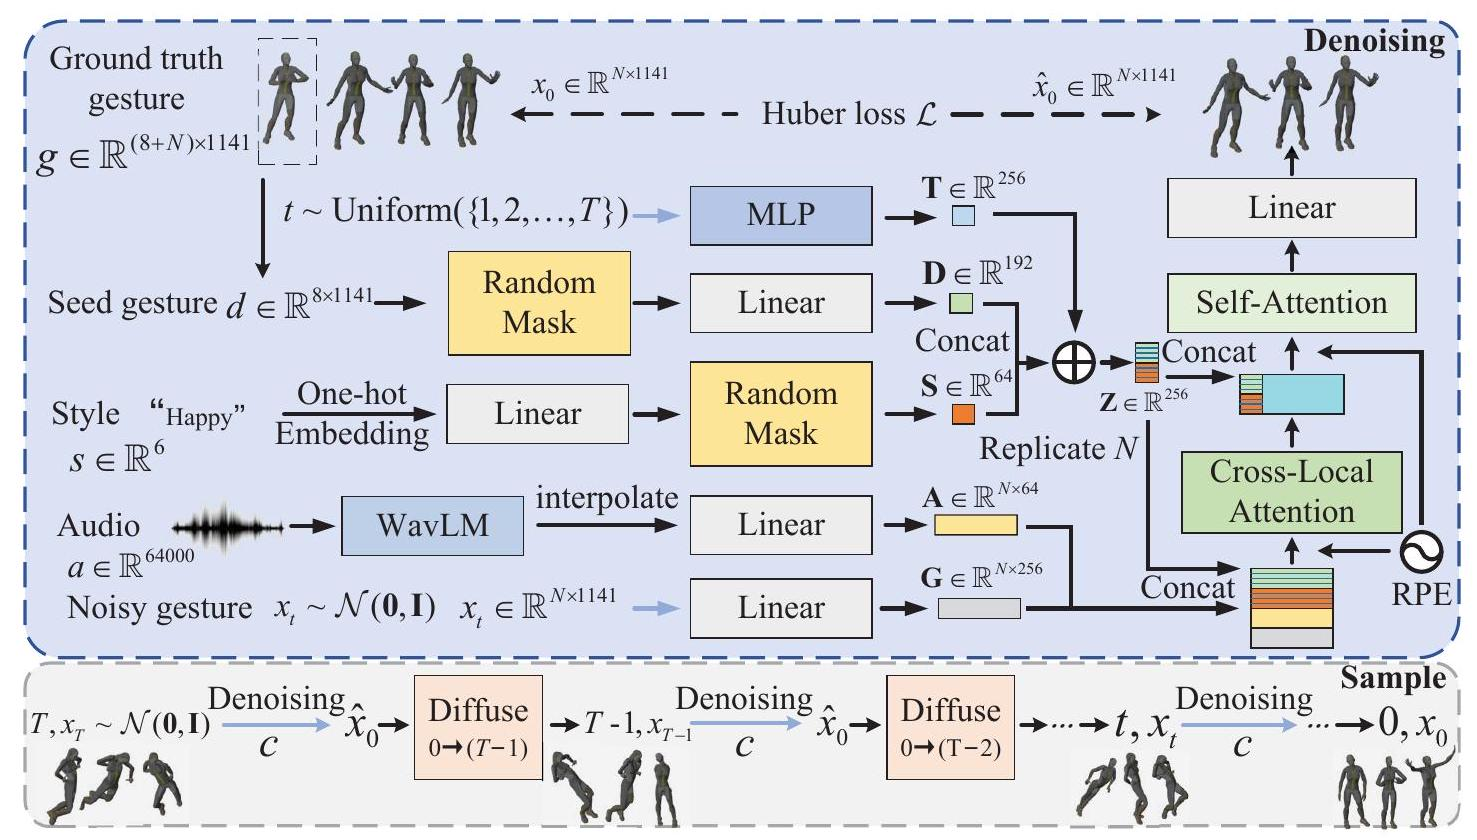
\includegraphics[width=\linewidth]{images/architecture.jpg}
%    \caption{Kiến trúc mồ hình sinh cử chỉ OHGesture}
%    \label{fig:architecture}
%\end{figure}

Trước tiên chúng tôi trình bày chúng tôi trình bày tổng quan của mô hình \ref{Overview},  và khung xương trong mỗi khung hình \ref{Skeleton} để hiểu được dữ liệu của mỗi khung hình. Từ đó chúng tôi đề xuất cách có thể trích xuất các đặc trưng về pha \ref{PeriodicAutoencoder} của mỗi khung hình để từ đó cách dùng mạng học sâu để học và điều khiển chuyển động của khung hình dựa trên pha \ref{MotionControllers}.

\section{Tổng quan mô hình}
\label{Overview}

Mô hình của chúng tôi sẽ lấy dữ liệu đầu vào ở khung hình thứ $i$ và dự đoán khung hình thứ $i+1$. Dữ liệu của mỗi khung hình là một chuỗi $\tau$ Chúng tôi sẽ trình bày 
% 

\subsection{Kiến trúc khung xương của mô hình}
\label{Skeleton}

Mỗi khung xương (skeleton) bao gồm $75$ khớp (joins) được đặt tên và minh hoạ ở hình \ref{fig:Skeleton}. 

\begin{figure}[htbp]
	\centering
	\begin{subfigure}{0.45\textwidth}
		\centering
		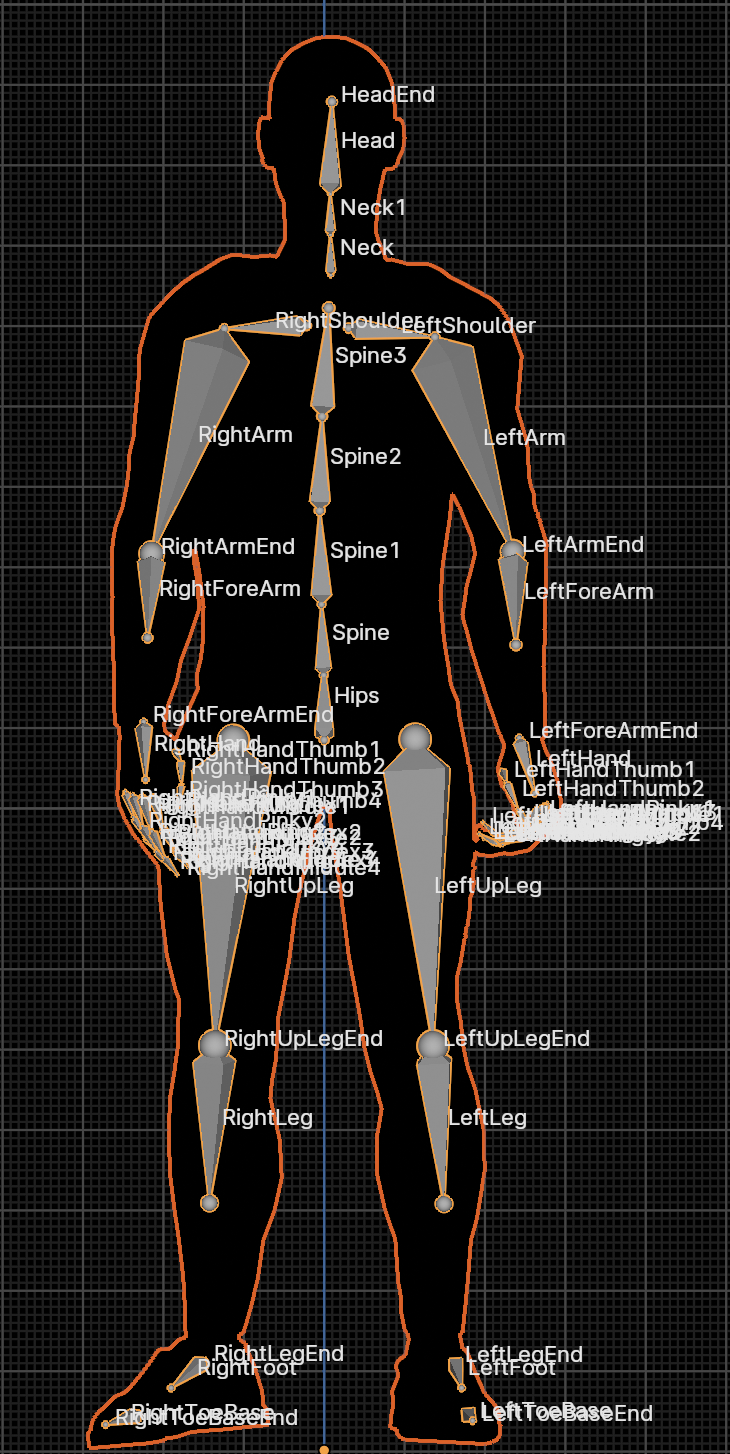
\includegraphics[height=10cm]{images/Skeleton.png}
		\caption{Khung xương và tên của các khớp của một khung xương trong mỗi khung hình.}
		\label{fig:Skeleton}
	\end{subfigure}
	\hfill
	\begin{subfigure}{0.45\textwidth}
		\centering
		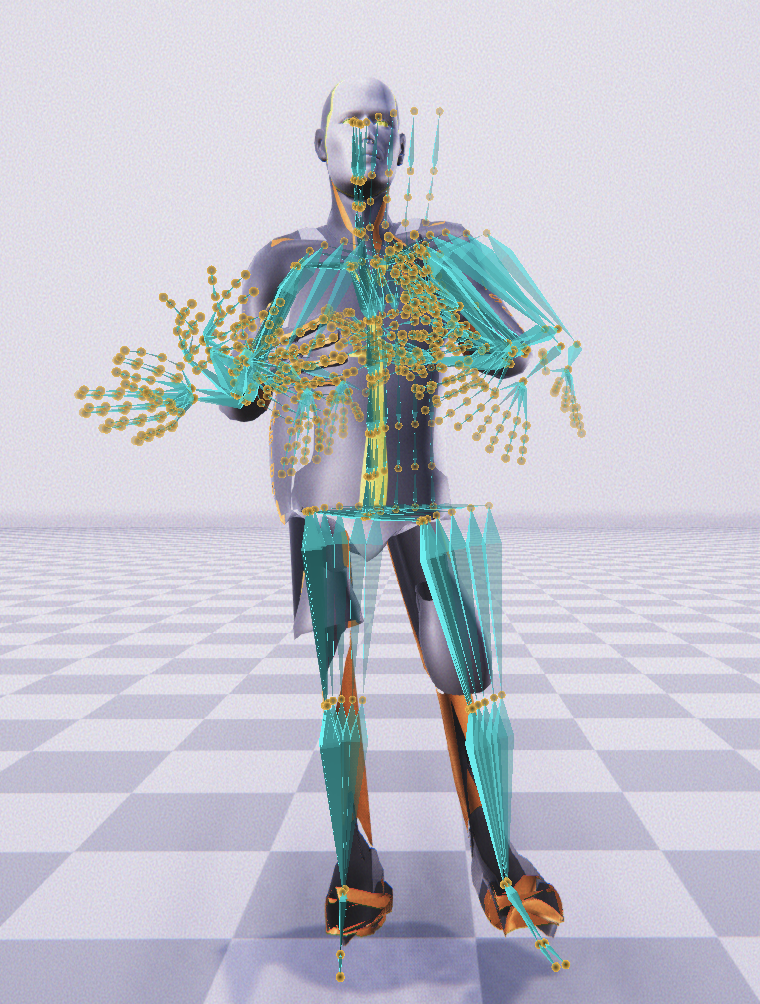
\includegraphics[height=10cm]{images/MotionPastAndFuture.png}
		\caption{Chuỗi chuyển động của cử chỉ bao gồm 6 cử chỉ quá khứ và 6 cử chỉ tương lai.}
		\label{fig:MotionPastAndFuture}
	\end{subfigure}
\end{figure}


\subsection{Đầu vào và đầu ra của mô hình}
\label{System}

%\begin{figure}
%	\centering
%	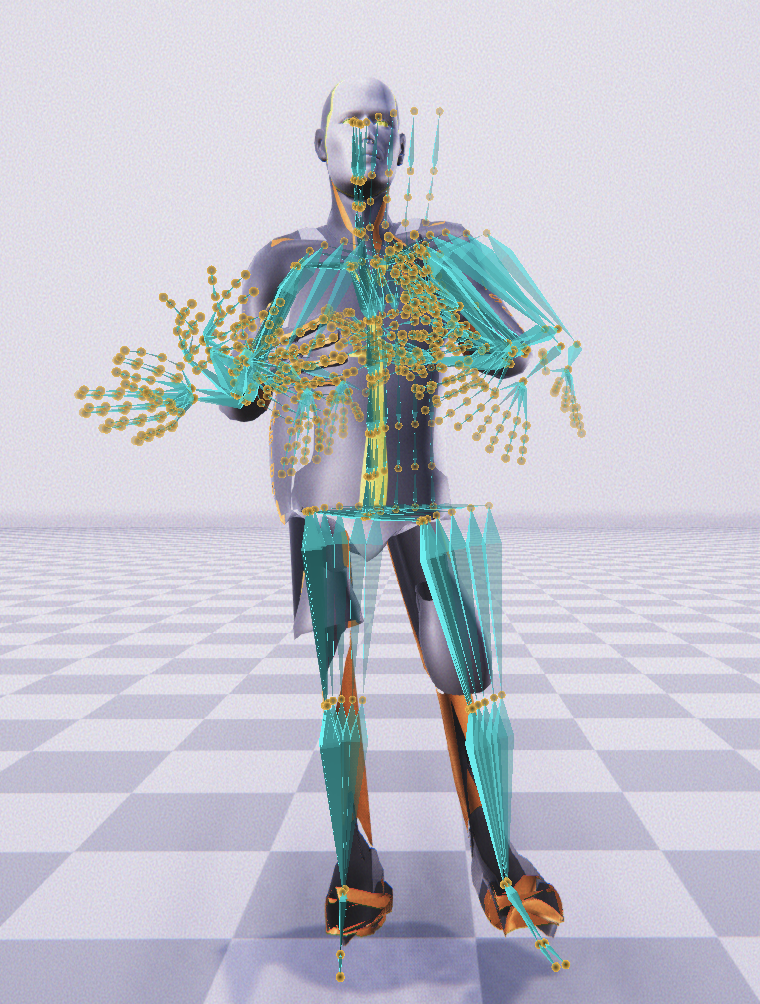
\includegraphics[height=10cm]{images/MotionPastAndFuture.png}
%	\caption{Các tham số đã học cho pha.}
%	\label{fig:MotionPastAndFuture}
%\end{figure}


\begin{figure}
	\centering
	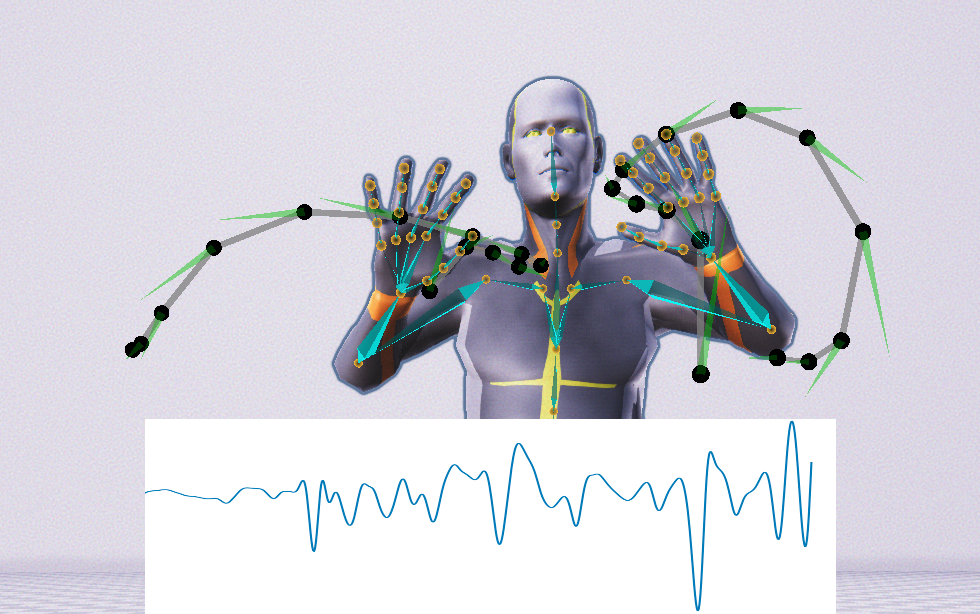
\includegraphics[height=10cm]{images/MotionSeries.png}
	\caption{Các tham số đã học.}
	\label{fig:MotionSeries}
\end{figure}

Hệ thống của chúng tôi là một mô hình chuỗi thời gian dự đoán các biến trạng thái của nhân vật, quả bóng, v.v. trong khung hình tiếp theo $i + 1$ dựa trên các biến trong khung hình hiện tại $i$. Các đầu vào và đầu ra được thiết kế sao cho hệ thống của chúng tôi có thể tạo ra các tương tác gần gũi giữa nhân vật và một đối tượng, một môi trường và một nhân vật khác. Một số biến cho điều khiển và điều kiện là hướng ứng dụng: ở đây, chúng tôi chủ yếu mô tả trong thiết lập bóng rổ, mặc dù khái niệm này là chung và có thể áp dụng cho các chuyển động khác như các thao tác của đối tượng và tương tác với môi trường. Để đào tạo, các đặc trưng Cartesian trong đầu vào và đầu ra được chuyển đổi vào hệ tọa độ gốc của nhân vật tại khung hình $i$ và $i + 1$, tương ứng. Tất cả các đặc trưng sống trong một cửa sổ chuỗi thời gian dài 1 giây, trong đó dữ liệu của 13 điểm mẫu đồng đều (6 điểm trong tương lai và 6 điểm trong quá khứ trong cửa sổ 1 giây, và một điểm cho khung hình hiện tại) được thu thập. Cách các giá trị được trích xuất từ dữ liệu ghi hình chuyển động được giải thích trong Phụ lục A.1.

\textbf{Inputs.} Vectơ đầu vào hoàn chỉnh $\textbf{X}_i$ tại khung hình $i$ bao gồm năm thành phần $\textbf{X}_i = \{ \textbf{X}^S_i, \textbf{X}^V_i, \textbf{X}^F_i, \textbf{X}^R_i, \textbf{X}^P_i \}$ trong đó mỗi thành phần được mô tả như dưới đây.

\begin{itemize}
	\item \textbf{Trạng thái Nhân vật}: \(\textbf{X}^\textbf{S}_i = \{p_i, r_i, v_i\}\) đại diện cho trạng thái của nhân vật của chúng tôi với \(B = 26\) xương tại khung hình hiện tại \(i\). Nó bao gồm các vị trí xương \(p_i \in \mathbb{R}^{3B}\), các xoay xương \(r_i \in \mathbb{R}^{6B}\) và vận tốc xương \(v_i \in \mathbb{R}^{3B}\), trong đó mỗi xoay xương được định nghĩa bằng cặp vector Cartesian tiến và lên của nó để tạo ra một không gian nội suy rõ ràng và liên tục.
	\item \textbf{Phase Chuyển Động Địa Phương} $\textbf{X}^{\mathcal{P}_i} = \Theta_i \in \mathbb{R}^{2KT}$ được đại diện bởi các vectơ pha 2D có biên độ thay đổi cho \(K = 5\) xương chính cho chân, tay và quả bóng, và được lấy mẫu dọc theo cửa sổ chuỗi thời gian từ quá khứ đến tương lai $T_{1s}^{-1s} = 13$. Các chi tiết về pha cấp xương được mô tả trong Phần 5.
	\item Third item
\end{itemize}

\textbf{Outputs} : Vector đầu ra $\textbf{Y}_i = \{ \textbf{Y}^S_i, \textbf{Y}^V_i, \textbf{Y}^F_i, \textbf{Y}^R_i, \textbf{Y}^P_i \}$ cho khung hình $i+1$

\section{Periodic Autoencoder}
\label{PeriodicAutoencoder}
%PERIODIC AUTOENCODER
	
\subsection{Network Structure}

\begin{figure}
    \centering
    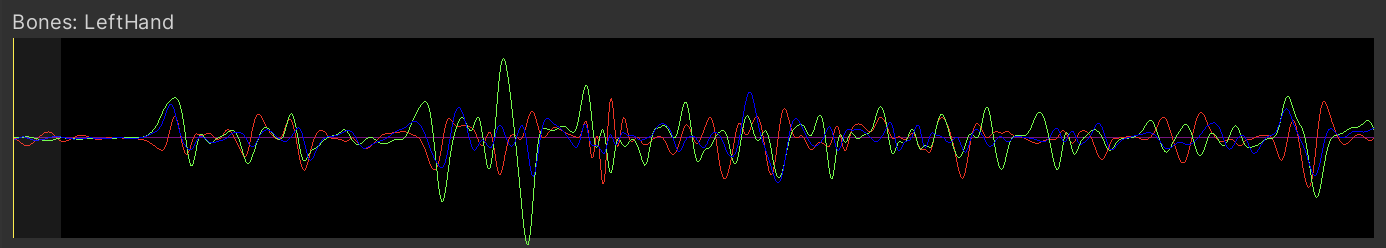
\includegraphics[width=\linewidth]{images/BoneRotationSeries.png}
    \caption{Minh hoạ sự thay đổi góc quay của một khung xương}
    \label{fig:BoneRotationSeries}
\end{figure}

Để biến đổi không gian chuyển động thành một đa tạp pha học được, chúng tôi sử dụng kiến trúc autoencoder tích chập theo thời gian tương tự như Holden và cộng sự [2015]. Tuy nhiên, ngoài việc huấn luyện mô hình để tái tạo đầu vào, chúng tôi còn bắt buộc mỗi kênh của không gian tiềm ẩn phải có dạng hàm tuần hoàn, điều này cho phép chúng tôi học một biến pha cho mỗi kênh tiềm ẩn từ một tập hợp nhỏ các tham số. Kiến trúc mạng của chúng tôi được hiển thị trong Hình 2. Dữ liệu theo thời gian được chia thành các cửa sổ chồng chéo nhau với độ dài $N$ và cửa sổ thời gian trung tâm tương ứng là $T$. Với các đường cong chuyển động đầu vào, $X \in \mathbb{R}^{D \times N}$, trong đó $D$ là số bậc tự do của cơ thể và $N$ là số khung hình của $X$, chúng tôi huấn luyện một bộ mã hóa, $g$, sử dụng các tích chập 1D để học một nhúng không gian thấp hơn của chuyển động.


\begin{equation}
	\label{eq:encoder}
	\mathbf{L} = g( \textbf{X} )
\end{equation}

Giả sử $L \in \mathbb{R}^{M \times N}$, trong đó $M$ là số kênh tiềm ẩn, tức là số kênh pha mong muốn được trích xuất từ chuyển động. Chúng tôi áp đặt tính chu kỳ bằng cách tham số hóa mỗi đường cong tiềm ẩn trong $\mathbf{L}$ dưới dạng một hàm sóng hình sin, được xác định bởi các tham số biên độ ($\mathbf{A}$), tần số ($\mathbf{F}$), độ lệch ($\mathbf{B}$) và dịch pha ($\mathbf{S}$).

Để tính toán $\mathbf{A}, \mathbf{F}, \mathbf{B} \in \mathbb{R}^{M}$, chúng tôi sử dụng một lớp Fast Fourier Transform (FFT) thực khả vi. Chúng tôi áp dụng FFT cho mỗi kênh của $\mathbf{L}$ và tạo ma trận hệ số Fourier có chỉ mục bằng không $\mathbf{c} \in \mathbb{C}^{M \times (K+1)}, K=\left\lfloor \frac{N}{2} \right\rfloor$.

\begin{equation}
	\label{eq:fft}
	\mathbf{c}=F F T(\mathbf{L}), \quad \mathbf{p}_{i, j}=\frac{2}{N}\left|\mathbf{c}_{i, j}\right|^2
\end{equation}

trong đó $i$ là chỉ số kênh và $j$ là chỉ số cho các dải tần số. Các tham số tương ứng sau đó được cho bởi


\begin{equation}
	\label{eq:PhaseExtraction}
	\mathbf{A}_i=\sqrt{\frac{2}{N} \sum_{j=1}^K \mathbf{p}_{i, j}}, \quad \mathbf{F}_i=\frac{\sum_{j=1}^K\left(\mathbf{f}_j \cdot \mathbf{p}_{i, j}\right)}{\sum_{j=1}^K \mathbf{p}_{i, j}}, \quad \mathbf{B}_i=\frac{\mathbf{c}_{i, 0}}{N}
\end{equation}

trong đó $\textbf{f} = (0, \frac{1}{T}, \frac{2}{T}, \dots, \frac{K}{T})$ là một vector các tần số. Các phép toán này cung cấp các tham số hình dạng để xây dựng $M$ hàm tuần hoàn trong khoảng thời gian, nhưng chưa bao gồm yếu tố thời gian, tức là các dịch pha của các hàm này. Để có được tham số thời gian này, chúng tôi học một lớp fully-connected (FC) riêng biệt cho mỗi đường cong tiềm ẩn, lớp này chỉ dự đoán dịch pha có dấu $\textbf{S} \in \mathbb{R}^{M}$ tại khung trung tâm của $T$ thông qua một vector trung gian hai chiều:

\begin{equation}
	\label{eq:OffsetExtraction}
	\left(s_x, s_y\right)=F C\left(\mathrm{~L}_i\right), \quad \mathrm{S}_i=\operatorname{atan} 2\left(s_y, s_x\right)
\end{equation}

trong đó $i$ là chỉ số kênh.

Từ các tham số đã học được $F$, $A$, $B$ và $S$, cùng với khoảng thời gian $T$ đã biết, ta có thể tái tạo không gian tiềm ẩn được tham số hóa $\hat{L}$ dưới dạng nhiều hàm tuần hoàn có cùng dạng kích thước như không gian tiềm ẩn ban đầu bằng cách sử dụng hàm tham số hóa $f$:

\begin{equation}
	\label{eq:Sinusoidal}
	\hat{\mathbf{L}}=f(\mathcal{T} ; \mathbf{A}, \mathbf{F}, \mathbf{B}, \mathbf{S})=\mathbf{A} \cdot \sin (2 \pi \cdot(\mathbf{F} \cdot \mathcal{T}-\mathbf{S}))+\mathbf{B}
\end{equation}


Cuối cùng, mạng giải mã không gian tiềm ẩn đã được tham số hóa bằng các phép deconvolution 1D trong bộ giải mã $h$, để ánh xạ trở lại các đường cong chuyển động đầu vào ban đầu:

\begin{equation}
	\label{eq:Decoder}
	\textbf{Y} = h(\hat{\textbf{L}})
\end{equation}

Mạng được huấn luyện bằng hàm mất mát tái tạo giữa các đường cong chuyển động gốc và dự đoán:

\begin{equation}
	\label{eq:LossFunction}
	\mathcal{L} = \text{MSE}(\textbf{X}, \textbf{Y})
\end{equation}

Điều này buộc mạng phải học sự căn chỉnh thời gian của các tư thế trên các đoạn clip chuyển động khác nhau và gán một pha thay đổi cho mỗi khung hình mới của chuyển động theo một hướng nhất định. Để thấy điều này, hãy xem xét một đoạn chuyển động có khung trung tâm tại thời điểm $t$, được trích xuất từ một đoạn clip chuyển động dài hơn và được mã hóa để tạo ra $\hat{\textbf{L}}$. Các tham số $\textbf{A}$, $\textbf{F}$ và $\textbf{B}$ giới hạn hình dạng của các tín hiệu tuần hoàn và mạng phải học cách định vị các đường cong chính xác bằng $\textbf{S}$. Đối với một đoạn chuyển động có khung trung tâm tại thời điểm $t + 1$, được trích xuất từ cùng một đoạn clip chuyển động, chúng ta kỳ vọng rằng mọi thay đổi trong $\textbf{A}$, $\textbf{F}$ và $\textbf{B}$ sẽ rất nhỏ (xem Hình 3), vì vậy $\textbf{S}$ cần phải tiến triển để giữ cho không gian tiềm ẩn đồng bộ với chuyển động, vì cùng một bộ giải mã tích chập được sử dụng. Điều này có nghĩa là mô hình phải học cách dự đoán các vector 2D quay theo chiều kim đồng hồ để thay đổi các giá trị của biểu diễn tuần hoàn mà từ đó nó cần tái tạo các đường cong đầu vào.

Một cách khác để xây dựng đa tạp pha là học các tham số tuần hoàn trực tiếp bằng mạng thay vì sử dụng lớp FFT: chúng tôi đã thử nghiệm điều này nhưng không chỉ tham số pha mà cả biên độ và tần số cũng dao động rất nhiều theo thời gian, dẫn đến một đa tạp pha rất nhiễu. Việc học chuyển đổi tín hiệu sang miền tần số dường như không dễ dàng, và sử dụng lớp FFT làm ổn định quá trình học đáng kể.

\begin{figure}
	\centering
	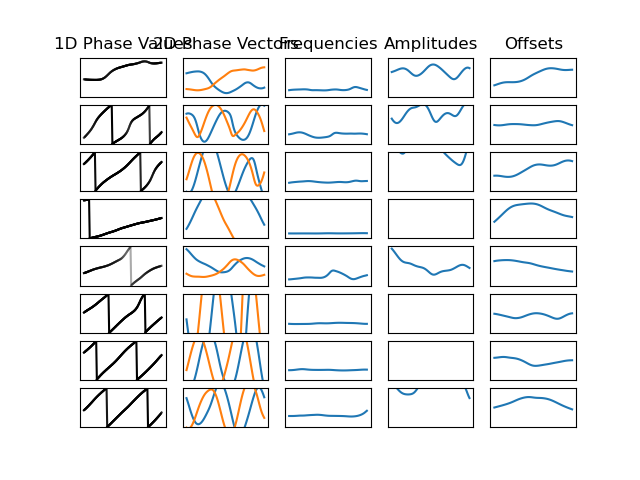
\includegraphics[width=\linewidth]{images/phase_bias_frequency_amplitudes_offsets.png}
	\caption{Các tham số đã học cho pha, biên độ, tần số và độ lệch cho một khoảng thời gian chuyển động cố định trong quá trình huấn luyện mạng để tái tạo chuyển động đầu vào, và từ đó có thể xây dựng đa tạp pha.}
	\label{fig:phase_bias_frequency_amplitudes_offsets}
\end{figure}

%$$
%\Gamma(x) = A sin (2 \pi (Fx - S)) + B
%$$

%Diffusion \cite{ho2020denoising} là mô hình được lấy cảm hứng từ mô hình khuếch tán các chất trong hóa học.

\subsection{Phase Manifold}
\label{sec:summary_diffusion}

%\begin{figure*}
%	\centering
%	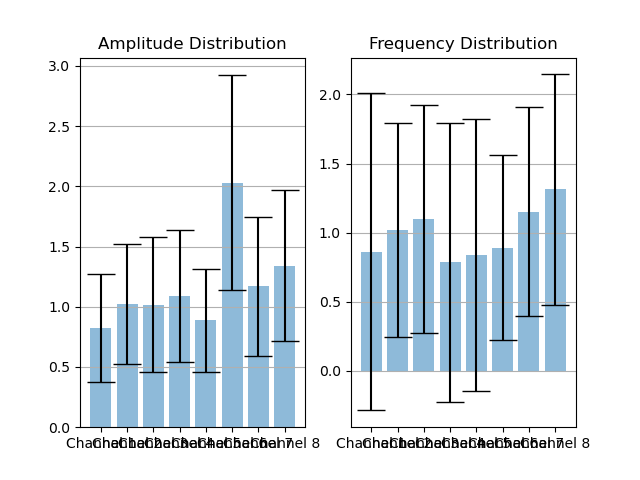
\includegraphics[width=0.8\linewidth]{images/distribution.png}
%	\caption{Phân phối của các biên độ và tần số của các kênh pha đã học. Mỗi kênh được điều chỉnh cho một khoảng biên độ và tần số cụ thể để phân tích chuyển động, hoạt động như một tập hợp các bộ lọc thông dải đã học. Lưu ý rằng không có các khoảng tham số được định nghĩa trước cho mỗi kênh pha, mà chúng được trích xuất theo nhu cầu của mô hình.}
%	\label{fig:distribution}
%\end{figure*}

\begin{figure}
	\centering
	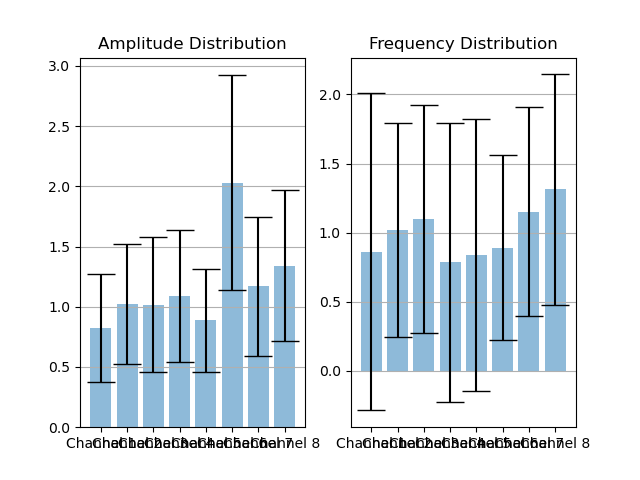
\includegraphics[height=10cm,width=\linewidth]{images/distribution.png}
	\caption{Phân phối của các biên độ và tần số của các kênh pha đã học. Mỗi kênh được điều chỉnh cho một khoảng biên độ và tần số cụ thể để phân tích chuyển động, hoạt động như một tập hợp các bộ lọc thông dải đã học. Lưu ý rằng không có các khoảng tham số được định nghĩa trước cho mỗi kênh pha, mà chúng được trích xuất theo nhu cầu của mô hình.}
	\label{fig:distribution}
\end{figure}

Chúng tôi sẽ mô tả cách mà đa tạp pha được hình thành bằng cách sử dụng các biến tiềm ẩn chu kỳ được tính toán với Mạng Tự Động Hóa Chu Kỳ. Sau khi huấn luyện mạng, các tham số chu kỳ cho một tập dữ liệu chuyển động không có cấu trúc có thể được tính toán cho mỗi khung hình bằng cách dịch Mạng Tự Động Hóa Chu Kỳ dọc theo các đường cong chuyển động. Các tham số chu kỳ đại diện cho tính chu kỳ cục bộ của các biến tiềm ẩn: sử dụng chúng, chúng tôi hình thành một đa tạp pha $\mathcal{P}$ có kích thước $\mathbb{R}^{2M}$, trong đó một mẫu tại khung hình $t$ được tính bằng

\begin{equation}
	\label{eq:phase_define}
	\mathcal{P}^{(t)}_{2i-1} = \textbf{A}^{(t)}_i \cdot \sin(2\pi \cdot \textbf{S}^{(t)}_i), \quad \mathcal{P}^{(t)}_{2i} = \textbf{A}^{(t)}_i \cdot \cos(2\pi \cdot \textbf{S}^{(t)}_i)
\end{equation}


\begin{figure}
	\centering
	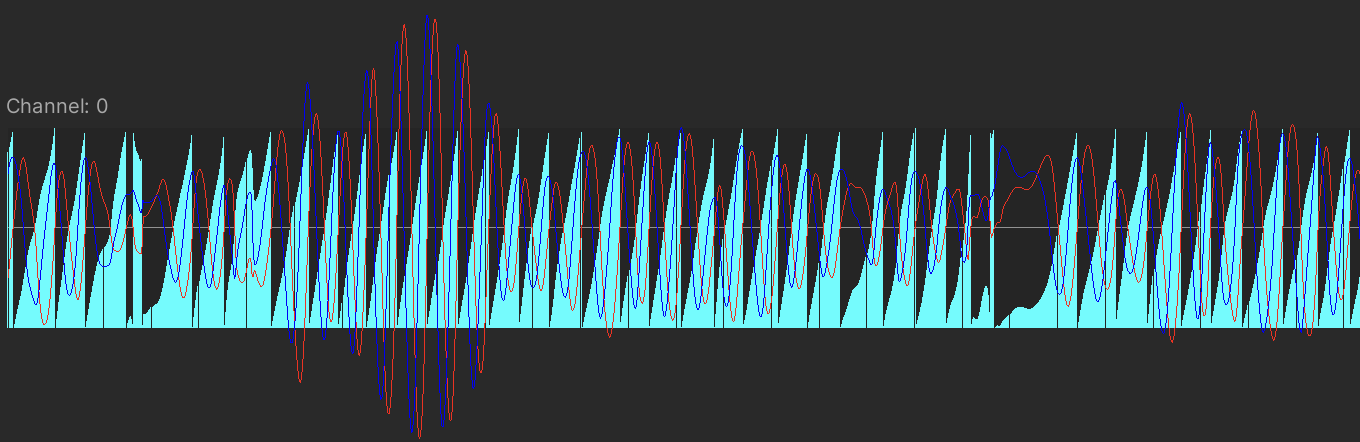
\includegraphics[width=\linewidth]{images/PhaseChannel.png}
	\caption{Phân phối của các biên độ và tần số của các kênh pha đã học. Mỗi kênh được điều chỉnh cho một khoảng biên độ và tần số cụ thể để phân tích chuyển động, hoạt động như một tập hợp các bộ lọc thông dải đã học. Lưu ý rằng không có các khoảng tham số được định nghĩa trước cho mỗi kênh pha, mà chúng được trích xuất theo nhu cầu của mô hình.}
	\label{fig:PhaseChannel}
\end{figure}


Các đặc trưng trong $\mathcal{P}$ mô tả tốt thời gian của khung hình trong chuyển động đầu vào $\textbf{X}$ và giúp rất nhiều trong việc căn chỉnh các chuyển động trong cùng một lớp hoặc giữa các lớp chuyển động khác nhau. Điều này có nghĩa là chúng có thể hoạt động hiệu quả như một đặc trưng đầu vào cho việc tổng hợp chuyển động thần kinh hoặc so khớp chuyển động, chúng tôi sẽ trình bày cách sử dụng và kết quả trong Mục 4 và Mục 5. Các biến pha của mười kênh trong một khoảng thời gian ngắn cho một đoạn clip chuyển động ví dụ được vẽ trong Hình 3. Có thể quan sát rằng mỗi kênh học các đặc trưng cho các tần số khác nhau, tương ứng với các tốc độ chuyển động khác nhau. Chúng tôi vẽ phân phối các biên độ và tần số của mỗi kênh trong Hình 4. Chúng tôi có thể quan sát rằng mỗi kênh pha học cách trích xuất các khoảng giá trị biên độ và tần số khác nhau trong các chuyển động. Hệ thống có thể mã hóa các chi tiết hoặc mẫu chuyển động khác nhau, điều này rất hữu ích cho việc căn chỉnh theo thời gian.

Khi có một chuỗi chuyển động, đặc trưng chu kỳ chuyển động mượt mà qua đa tạp pha. Vì biên độ và tần số của mỗi kênh pha có thể thay đổi theo thời gian, Mạng Tự Động Hóa Chu Kỳ có thể mã hóa các chuyển động không chu kỳ cũng như các chuyển động chu kỳ, chẳng hạn như chuyển tiếp từ một loại chuyển động này sang loại khác. Những chuyển tiếp không chu kỳ hoặc hành vi chuyển động như vậy có thể được quan sát dưới dạng biên độ tăng hoặc giảm cho các kênh khác nhau (ví dụ: một người đi bộ và bắt đầu vẫy tay), hoặc thay đổi không đồng bộ trong dịch pha hoặc tần số (ví dụ: chuyển tiếp giữa bước đi và bước chạy cho các loài bốn chân). Hình 5 minh họa những ví dụ như vậy nơi các pha có thể thể hiện các mẫu chu kỳ hoặc không chu kỳ trong suốt một đoạn clip chuyển động.



Lý do để định nghĩa đa tạp pha như trong phương trình (8) thay vì sử dụng riêng biệt tất cả các tham số như tần số, biên độ và pha là vì chúng tôi mong muốn các đặc trưng pha nhóm các hoạt ảnh theo cả không gian và thời gian. Các đặc trưng như tần số và biên độ vẫn gần như không thay đổi theo thời gian, và không giúp ích nhiều cho mục đích căn chỉnh. Biến đổi chúng thành một không gian hình cầu siêu thông qua phương trình (8) đạt được sự căn chỉnh không gian-thời gian như vậy, trong đó $A$ và $S$ định nghĩa điểm trong không gian đó và $F$ có thể được đại diện bởi một cửa sổ của các điểm như vậy. Phép biến đổi này cũng xây dựng một không gian nội suy liên tục: Trong khi các giá trị pha 1D là không liên tục và có thể trở nên không xác định nếu không có chuyển động nào được thực hiện, việc mã hóa chúng dưới dạng các vector 2D cho phép chuyển tiếp về gốc của đa tạp tại biên độ bằng không.

\subsection{Network Training}

Để huấn luyện Mạng Tự mã hóa Chu kỳ, chúng tôi sử dụng các quỹ đạo vận tốc khớp 3D làm đầu vào cho mạng, mỗi quỹ đạo được chuyển đổi vào không gian gốc của nhân vật [Holden et al. 2017]. Chúng tôi trừ đi giá trị trung bình dựa trên cửa sổ để căn giữa các đường cong chuyển động, nhưng không áp dụng bất kỳ phép tỷ lệ độ lệch chuẩn nào nhằm duy trì các khác biệt tương đối. Dữ liệu đầu vào bao gồm 60 khung hình (1 giây) mỗi khung ở quá khứ và tương lai xung quanh khung giữa với tần số 60 Hz. Điều này tạo ra một vector đầu vào $\textbf{X} \in \mathbb{R}^{3 \cdot J \times N}$, trong đó $J$ là số lượng khớp của nhân vật và $N$ (= 121) là số lượng mẫu thời gian.
Đối với bộ mã hóa $g$, chúng tôi sử dụng hai lớp tích chập, tạo ra một ánh xạ $(3 \cdot J \times N) \to (J \times N) \to (M \times N)$, để tính toán nhúng đường cong chuyển động. Mỗi lớp tích chập được theo sau bởi một phép chuẩn hóa theo lô (batch normalization) và hàm kích hoạt tanh. Vì chúng tôi thực hiện trực tiếp các phép toán trên không gian tiềm ẩn để trích xuất các tham số chu kỳ, chúng tôi nhận thấy rằng việc chuẩn hóa theo lô giúp ổn định quá trình huấn luyện cho nhiệm vụ này và giúp ngăn chặn sự phân phối không gian tiềm ẩn bị suy giảm hoặc mô hình bị quá khớp khi được huấn luyện quá lâu. Chúng tôi cũng áp dụng một phép chuẩn hóa theo lô cho vector dịch pha dự đoán trước khi tính toán góc có dấu của nó. Bộ giải mã $h$ lại bao gồm hai lớp tích chập để tính toán một ánh xạ $(M \times N) \to (J \times N) \to (3 \cdot J \times N)$, nhưng chỉ áp dụng phép chuẩn hóa theo lô và hàm kích hoạt tanh sau lớp giải chập đầu tiên và không áp dụng cho lớp đầu ra. Chúng tôi huấn luyện mạng của mình bằng bộ tối ưu AdamW [Loshchilov và Hutter 2019] trong 30 epoch, sử dụng tốc độ học và độ suy giảm trọng số đều là $10^{-4}$ và kích thước lô là 32. Việc huấn luyện trên GPU NVIDIA RTX 3090 thường mất chưa đầy một giờ cho các tác vụ nhỏ hơn.


\section{Motion Controllers}
\label{MotionControllers}

\subsection{Neural Motion Controller}

\begin{figure}
	\centering
	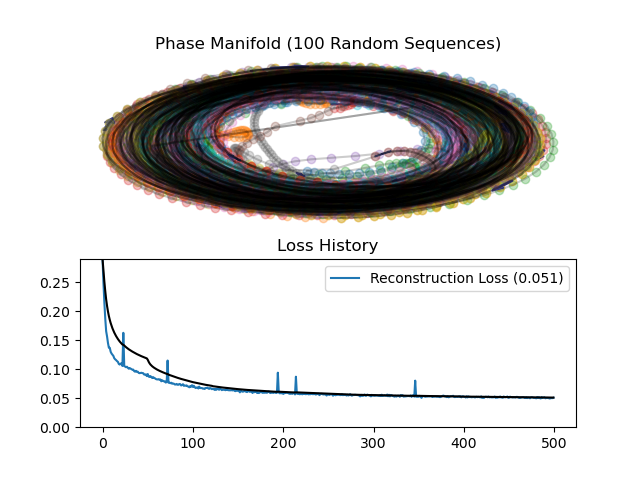
\includegraphics[]{images/PhaseManifold.png}
	\caption{Phân phối đặc trưng cho các miền chuyển động khác nhau trong không gian vận tốc (trên), không gian tiềm ẩn được học bởi mạng tích chập + mạng kết nối hoàn toàn (giữa) và không gian pha (dưới) được trực quan hóa bằng phép chiếu PCA 2D. Mỗi màu đại diện cho các tư thế từ một chuỗi chuyển động duy nhất mà được kết nối theo thời gian.}
	\label{fig:PhaseManifold}
\end{figure}


Đối với bộ điều khiển dựa trên mạng nơ-ron, chúng tôi phát triển một mô hình chuỗi thời gian dự đoán tư thế trong khung hình hiện tại dựa trên khung hình trước đó và các điều khiển của người dùng hiện tại. Mô hình được huấn luyện theo cách giám sát sử dụng dữ liệu ghi hình chuyển động. Chúng tôi sử dụng khung Mixture-of-Experts pha trộn trọng số tương tự như [Starke et al. 2020; Zhang et al. 2018], nhưng thay vì sử dụng các vận tốc hoặc pha địa phương dựa trên tiếp xúc làm đầu vào cho mạng gating, chúng tôi sử dụng các vectơ pha trên mặt phẳng pha (tức là, Eq. (8)) làm các đặc trưng đầu vào để tạo ra các chuyển động theo cách tự hồi quy. Việc cung cấp đặc trưng pha làm đầu vào giúp hệ thống căn chỉnh dữ liệu chuyển động theo dòng thời gian và cho phép nhân vật chuyển tiếp giữa các chuyển động một cách thực tế như chúng tôi đã trình bày trong Mục 5.

Hệ thống tự hồi quy cập nhật trạng thái pha của nhân vật cũng như chuyển động của nó. Hệ thống đầu tiên dự đoán các vectơ pha tiếp theo $P_{t+\Delta t}$, các biên độ $A_{t+\Delta t}$ và tần số $F_{t+\Delta t}$. Thay vì sử dụng trực tiếp các vectơ pha đã dự đoán, nó được cập nhật như sau:

\begin{equation}
	\label{eq:PhaseVector}
	\mathcal{P}_{t+\Delta t}^{\prime}=A_{t+\Delta t} \cdot I\left(R(\theta) \cdot \mathcal{P}_t, \mathcal{P}_{t+\Delta t}\right), \quad \theta=\Delta t \cdot 2 \pi \cdot F_{t+\Delta t}
\end{equation}

trong đó \(\Delta t\) là thời gian delta của khung hình, \(R\) là ma trận quay 2D, và \(I\) là nội suy tuyến tính hình cầu với trọng số 0.5 để cho phép pha trộn góc pha và độ lớn một cách riêng biệt. Việc cập nhật pha theo cách này buộc tần số tiến triển pha theo hướng mà mạng nơ-ron đã dự đoán. Tần số là một giá trị dương đồng nhất dễ dự đoán và giữ cho mạng di chuyển qua không gian pha theo một cách một chiều (xem Hình 6). Sơ đồ này ngăn chuyển động trở nên cứng nhắc hoặc bị kẹt theo thời gian, điều này là một vấn đề phổ biến được quan sát thấy đối với các bộ điều khiển nhân vật dựa trên dữ liệu.

Mạng gating chuyên gia học cách pha trộn 8 bộ trọng số chuyên gia và bao gồm hai lớp ẩn có kích thước 128. Mạng tạo chuyển động sử dụng hai lớp ẩn có kích thước 512. Tỉ lệ dropout được đặt thành 0.3, kích thước lô là 32, và cả tốc độ học và suy giảm trọng số đều được khởi tạo là \(10^{-4}\). Chúng tôi sử dụng bộ tối ưu AdamWR [Loshchilov và Hutter 2019] với lịch trình giảm nhiệt cosin và đặt số lần khởi động lại là 10, hệ số khởi động lại là 2.0, và huấn luyện mô hình trong 150 epoch. Việc huấn luyện mỗi mô hình yêu cầu từ 12 đến 48 giờ. Mạng được triển khai trong PyTorch và tạo ra một tệp ONNX có thể được chạy trong Unity để suy diễn bằng cách sử dụng thư viện Barracuda của nó.


\subsection{Motion Matching}

Trong bối cảnh của việc khớp chuyển động, các pha có thể được sử dụng theo cách tương tự như đối với các mạng nơ-ron và không yêu cầu thay đổi trong các quy trình công việc điển hình cho việc khớp chuyển động. Sự khác biệt chính là thay vì khớp các đặc trưng tư thế hoặc vận tốc có chiều cao hơn của trạng thái nhân vật hiện tại, hệ thống khớp các vectơ pha có chiều thấp hơn để tìm kiếm tư thế ở khung hình tiếp theo dựa trên các tín hiệu điều khiển của người dùng, chẳng hạn như quỹ đạo gốc. Chúng tôi trực quan hóa các đặc trưng pha và các đặc trưng vận tốc cho các chuyển động khác nhau trong Hình 6 (xem Mục 5.1 để biết thêm chi tiết). Khoảng cách Euclid giữa các điểm lân cận trong không gian pha liền kề với nhau là đồng nhất (hàng dưới cùng), điều này có nghĩa là các tư thế được khớp bởi việc khớp chuyển động sẽ có sự khác biệt tương tự về thời gian. Điều này cho phép

tổng hợp các chuyển tiếp chuyển động mượt mà và thực tế hơn với ít điều chỉnh tham số hơn, điều này không dễ dàng xảy ra khi khớp các đặc trưng tư thế Cartesian (hàng trên cùng) cần được chọn thủ công cho các khớp cụ thể (ví dụ: chân cho chuyển động) hoặc yêu cầu thêm bộ lọc.





%\subsection{Quá trình gây nhiễu (forward diffusion process)}
%
%Cho dữ liệu $x_{0}$ là được lấy từ dữ liệu thật $x_{0} \sim q(x)$, với mỗi bước ta sẽ thêm nhiễu vào đầu vào $x_{0}$ với tỷ lệ nhiều và ảnh gốc được kiểm soát bằng hệ số $\beta$:
%
%
%\begin{equation}
%	\label{eq:addgaussian}
%	\mathbf{x}_t = \sqrt{1 - \beta_t}\mathbf{x}_{t-1} + \sqrt{\beta_t} \boldsymbol{\epsilon}_{t-1}
%\end{equation}
%
%Trong đó, quá trình gây nhiễu từ $1 \to T$, với mỗi bước $t$ quá trình thêm nhiễu $\epsilon$ được điều khiển bằng $\beta_t$ theo phương sai $\{\beta_t \in (0, 1)\}_{t=1}^T$:
%
%\begin{equation}
%	\label{eq:forward_diffusion_process}
%	\begin{aligned}
%		q(\mathbf{x}_t \vert \mathbf{x}_{t-1}) &= \mathcal{N}(\mathbf{x}_t; \sqrt{1 - \beta_t} \mathbf{x}_{t-1}, \beta_t\mathbf{I}) \quad \\
%		q(\mathbf{x}_{1:T} \vert \mathbf{x}_0) &= \prod^T_{t=1} q(\mathbf{x}_t \vert \mathbf{x}_{t-1})
%	\end{aligned}
%\end{equation}
%
%Mục tiêu ở bước $t$ của hệ số $\sqrt{1 - \beta_t}$ và $\beta_t$ là để lần lượt giảm tỷ lệ của ảnh gốc $x_t$ và tăng dần nhiễu  $\boldsymbol{\epsilon}_{t-1}$, vì vậy $\beta_1 < \beta_2 < \dots < \beta_T$. Khi $T \to \infty$ thì $x_{T}$ sẽ hoàn toàn nhiễu (Isotropic Gaussian Distribution).
%
%
%Vì nhiễu $\boldsymbol{\epsilon}_{t-1}, \boldsymbol{\epsilon}_{t-2}, \dots \sim \mathcal{N}(\mathbf{0}, \mathbf{I})$ luôn luôn là phân phối chuẩn, và cho trước trong mọi bước $t$, nên ta có thể dễ dàng truy ngược được $x_t$ từ $x_0$. Bằng cách đặt $\alpha_t = 1 - \beta_t$ và $\bar{\alpha}_t = \prod_{i=1}^t \alpha_i$, từ công thức \ref{eq:addgaussian}, ta có hàm forward diffusion viết lại theo $\alpha$ như sau:
%
%\begin{equation}
%	\label{eq:tracexzero}
%	\begin{aligned}
%		\mathbf{x}_t 
%		&= \sqrt{\alpha_t}\mathbf{x}_{t-1} + \sqrt{1 - \alpha_t}\boldsymbol{\epsilon}_{t-1} \\
%		&= \sqrt{\alpha_t \alpha_{t-1}} \mathbf{x}_{t-2} + \sqrt{1 - \alpha_t \alpha_{t-1}} \bar{\boldsymbol{\epsilon}}_{t-2}
%		&= \sqrt{\bar{\alpha}_t}\mathbf{x}_0 + \sqrt{1 - \bar{\alpha}_t}\boldsymbol{\epsilon} \\
%		q(\mathbf{x}_t \vert \mathbf{x}_0) &= \mathcal{N}(\mathbf{x}_t; \sqrt{\bar{\alpha}_t} \mathbf{x}_0, (1 - \bar{\alpha}_t)\mathbf{I})
%	\end{aligned}
%\end{equation}
%
%
%\subsection{Quá trình khử nhiễu (denoising process)}
%\label{subsection:denoising_process}
%
%Quá trình khử nhiễu $p_\theta(\mathbf{x}_{t-1} \vert \mathbf{x}_t)$  ở bước thứ $t$ từ $T \to 1$ được bắt đầu từ $x_T$ là hoàn toàn nhiễu $\mathcal{N} (\mathbf{0}, \mathbf{I})$. Ta sẽ dùng một neural network $f_{\theta} (x_t, t)$ để dự đoán nhiễu $\hat{\epsilon} = f_{\theta}(x_t, t)$ đã được thêm vào để được $x_{t-1}$ từ $x_t$.
%. Quá trình khử nhiễu có trung bình $\boldsymbol{\mu}_\theta(\mathbf{x}_t, t) = {\frac{1}{\sqrt{\alpha_t}} \Big( \mathbf{x}_t - \frac{1 - \alpha_t}{\sqrt{1 - \bar{\alpha}_t}}  f_\theta(\mathbf{x}_t, t) \Big)}$ và độ lệch chuẩn $\boldsymbol{\Sigma}_\theta(\mathbf{x}_t, t)$ như sau:
%
%
%%\begin{equation} \mathrm{d}\mathbf{x} = [\mathbf{f}(\mathbf{x}, t) - g^2(t) \nabla_\mathbf{x} \log p_t(\mathbf{x})]\mathrm{d}t + g(t) \mathrm{d} \mathbf{w}.\label{rsde} \end{equation}
%
%% bằng cách lấy ảnh bị nhiễu trừ đi nhiễu dự đoán
%
%\begin{equation}
%	\label{eq:denoising_process}
%	\begin{aligned}
%		p_\theta(\mathbf{x}_{0:T})
%		&= p(\mathbf{x}_T) \prod^T_{t=1} p_\theta(\mathbf{x}_{t-1} \vert \mathbf{x}_t) \\
%		p_\theta(\mathbf{x}_{t-1} \vert \mathbf{x}_t) &= \mathcal{N}(\mathbf{x}_{t-1};  \boldsymbol{\mu}_\theta(\mathbf{x}_t, t), \boldsymbol{\Sigma}_\theta(\mathbf{x}_t, t))
%	\end{aligned}
%\end{equation}
%
%%Ta viết lại hàm denoising từ công thức \ref{eq:denoising_process}  theo $\alpha$ như sau:
%%$$
%%x_{t-1} = \frac{1}{\sqrt{\alpha_t}} \left( x_t - \frac{\sqrt{1 - \alpha_t}}{\sqrt{1 - \bar{\alpha}_t}} \epsilon_{\theta}(x_t, t) \right) + \sqrt{1 - \alpha_t} \tilde{\epsilon}_t
%%$$
%
%
%%\begin{equation}
%%	\label{eq:denoising_alpha}
%%	\begin{aligned}
%	%	p_\theta(\mathbf{x}_{t-1} \vert \mathbf{x}_t) &= \mathcal{N}(\mathbf{x}_{t-1}; \boldsymbol{\mu}_\theta(\mathbf{x}_t, t), \boldsymbol{\Sigma}_\theta(\mathbf{x}_t, t))
%	%\end{aligned} \\
%	% \bar{\boldsymbol{\mu}}_t (x_t, t) = \frac{1}{\sqrt{\alpha_t}} \Big( \mathbf{x}_t - \frac{1 - \alpha_t}{\sqrt{1 - \bar{\alpha}_t}} \boldsymbol{\epsilon}_t \Big)
%	%\end{equation}
%	
%	\subsection{Hàm mất mát $\mathcal{L}$ của mô hình diffusion}
%	
%	Như đã trình bày ở trên, mô hình diffusion sẽ học trọng số $\theta$ của hàm dự đoán lỗi $f_{\theta} (x_t, t)$. Trong quá trình denoising, ta sẽ tối ưu độ lỗi giữa nhiễu dự đoán $\boldsymbol{\epsilon}_\theta(\mathbf{x}_t, t)$ và nhiễu thực tế $\boldsymbol{\epsilon}_t$. Với mỗi bước thứ $t$ ta sẽ tối ưu hàm loss $\mathcal{L}_{t}$ để thu được trọng số $\theta$.
%	
%	\begin{equation}
%		\label{eq:diffusion_loss}
%		\begin{aligned}
%			\mathcal{L}_t
%			&= \mathbb{E}_{t \sim [1, T], \mathbf{x}_0, \boldsymbol{\epsilon}_t} \Big[\|\boldsymbol{\epsilon}_t - \boldsymbol{\epsilon}_\theta(\mathbf{x}_t, t)\|^2 \Big] \\
%			&= \mathbb{E}_{t \sim [1, T], \mathbf{x}_0, \boldsymbol{\epsilon}_t} \Big[\|\boldsymbol{\epsilon}_t - \boldsymbol{\epsilon}_\theta(\sqrt{\bar{\alpha}_t}\mathbf{x}_0 + \sqrt{1 - \bar{\alpha}_t}\boldsymbol{\epsilon}_t, t)\|^2 \Big]
%		\end{aligned}
%	\end{equation}
%	
%	Thay vì dùng neuron network để dự đoán phân bố của dữ liệu theo như hình \ref{fig:basic_diffusion}, mô hình diffusion sẽ dự đoán độ lỗi được thêm vào trong ảnh ở bước thứ $t$, với mỗi $t$ bước ta sẽ cần tối ưu hàm mất mát $\mathcal{L}_t$, hàm mất mát của mỗi bước sẽ tối ưu độ lỗi giữa nhiễu dự đoán $\hat{\epsilon_t}$ và nhiễu nhãn $\epsilon_t$ được thêm vào. Với $f_{\theta}(x_{t-1}, t)$ là một mô hình Unet dùng để mã hoá và giải mã dữ liệu để dự đoán nhiễu đã thêm vào dữ liệu.
%	
%	%Hàm loss
%	
%	
%	\subsection{Quá trình dự đoán trong mô hình diffusion}
%	
%	Sau khi thu được trọng số $\theta'$, ta sẽ dùng hàm denoising để khử nhiễu từ nhiễu $x_T \sim \mathcal{N} (\mathbf{0}, \mathbf{I})$.
%	Quá trình biến đổi từ nhiễu hoàn toàn $x_{T}$ sang dự đoán $\hat{x_0}$ như sau:
%	%với $t$ là một vector đã được nhúng vị trí bằng thuật toán nhúng
%	
%	\begin{equation}
%		\label{eq:adddenoising}
%		x_{t-1} = \frac{1}{\sqrt{\alpha_t}} \left( x_t - \frac{1- \alpha_t}{\sqrt{1 - \bar{\alpha}_t}} f_{\theta'}(x_t, t) \right) + \sqrt{1 - \alpha_t} \tilde{\epsilon}_t
%	\end{equation}
%	
%	Lưu ý rằng $\tilde{\epsilon}_t$ là nhiễu cố định $\epsilon_t$ giống với nhiễu trong quá trình forward diffusion \ref{subsection:denoising_process} ở công thức  \ref{eq:addgaussian}.
%
	
% GAT
%% \section*{Mô hình sinh cử chỉ OHGesture}

% \section*{3 Phương Pháp Của Chúng Tôi}
% Diffusion là mô hình đằng sau các thành công của  Stable Diffusion, Midjourney và DALL-E trong việc tạo ra các tấm ảnh siêu thực.


%. Biếm tiềm ẩm ở đây là cử chỉ và điều kiện là cảm xúc. 
%Kiến trúc của OHGesture được trình bày như hình \autoref{fig:diffusion_forward}.


\section{Mô hình của đề xuất OHGesture}
\label{sec:ohgesture}

\begin{figure}
	\centering
	\includegraphics[width=\linewidth]{images/diffusion_forward}
	\caption{Minh hoạ quá trình khử nhiễu (denoising) cử chỉ}
	\label{fig:diffusion_forward}
\end{figure}

Mô hình \textbf{OHGesture} của chúng tôi áp dụng mô hình khuếch tán \cite{ho2020denoising} với điều kiện \cite{ho2022classifier} (Classifier-Free Diffusion Guidance). Trong đó $x_0$ là chuỗi cử chỉ $g \in \mathbb{R}^{N \times 1141}$, với điều kiện $c$bao gồm  .
Với đầu vào bao gồm cử chỉ khởi tạo $x_{\text{seed}}$, âm thanh $a$ và văn bản $t$.
% với biến tiềm ẩn   (diffusion latent variable)
Mô hình diffusion bao gồm hai quá trình: quá trình tạo nhiễu (diffusion) $q$ và quá trình khử nhiễu (denoising process) $p_{\theta}$. 
Trước tiên chúng tôi trình bày trước về phương pháp nền tảng (baseline) của mô hình diffusion.

\subsection{Quá trình trích xuất đặc trưng}

Dữ liệu để học của chúng tôi được lấy từ tập dữ liệu BEAT (Body-Expression-Audio-Text)
\cite{liu2022beat}. Tương tự mô hình DiffuseStyleGesture \cite{yang2022DiffuseStyleGestureplus} chúng tôi cũng sử dụng đầu vào bao gồm âm thanh, cử chỉ và cảm xúc, ngoài ra chúng tôi sử dụng thêm dữ liệu văn bản.

\begin{itemize}
	\item \textbf{Cử chỉ}: Cử chỉ ground truth là dữ liệu bao gồm 75 khớp xương được trình bày ở công thức \ref{eq:gesturevector}. Chúng tôi cắt $N_{\text{seed}} = 8$ frame đầu để làm cử chỉ khởi tạo và $N$ frame tiếp theo làm cử chỉ để dự đoán theo âm thanh và văn bản.
	
%	\item\textbf{Âm thanh}: Âm thanh sẽ được dùng làm đặc trưng để sinh cử chỉ, Chúng tôi sử dụng các mô hình Pretrain có sẵn như WavLM \cite{chen2022wavlm} để trích xuất đặc trưng âm thanh. 
%	Chúng tôi kết hợp thêm các đặc trưng về MFCC, Mel-Spectrum, Pitch, Enery và Onsets \cite{bello2005tutorial}
  \item \textbf{Âm thanh}: Tất cả dữ liệu âm thanh được giảm số sample rate (downsampled) xuống $16 \mathrm{kHz}$ và các vector tiềm ẩn được lấy từ các mô hình pre-train của WavLM Large \cite{chen2022wavlm}. Chúng tôi sử dụng nội suy tuyến tính (interpolation) để căn chỉnh đặc trưng của vector tiềm ẩn trong WavLM và cử chỉ $x_{0}$ theo chiều thời gian thành $20fps$, sau đó sử dụng một lớp tuyến tính để giảm kích thước của đặc trưng xuống còn 64 tạo thành chuỗi đặc trưng âm thanh cuối cùng $\mathbf{A}$.
		
	\item \textbf{Cảm xúc}: Cảm xúc bao gồm 6 cảm xúc khác nhau được biểu diễn thành một vector theo phương pháp one-hot encoding.
	
	\item \textbf{Văn bản}: Văn bản được trích xuất thông qua mô hình FastText \cite{yoon2022genea} để lấy được vector word embedding.
	
	\item \textbf{Cử chỉ nhiễu} (Noisy gesture): khi huấn luyện, $x_{t}$ là cử chỉ nhiễu có cùng kích thước như cử chỉ gốc $x_{0}$ sẽ được sinh ngẫu nhiên từ phân phối chuẩn $\mathcal{N}(0, \mathbf{I})$. Khi sinh ngẫu nhiên, cử chỉ nhiễu ban đầu $x_{T}$ được lấy mẫu từ phân phối chuẩn tiêu chuẩn và các $x_{t}, t<T$ khác là kết quả của bước làm nhiễu trước đó. Sau đó, kích thước được điều chỉnh thành 256 như $\mathbf{G}$ bằng lớp linear.
	
\end{itemize}

%\item Bước làm nhiễu: Trong quá trình huấn luyện, bước làm nhiễu $t$ được lấy mẫu từ phân phối chuẩn của $\{1,2, \ldots, T\}$, với mã hóa vị trí (position encoding) giống như mô hình Transformer \cite{vaswani2017attention}, sau đó được ánh xạ vào không gian $\mathbf{T}$ có kích thước 256 bằng một mạng perceptron nhiều lớp (MLP).
%
%
%
%\item Cảm xúc: Các cảm xúc của cử chỉ được biểu diễn dưới dạng vectơ one-hot encoding, tức thành vector toàn bộ là số $0$ và vị trí có cảm xúc tương ứng có vị trí là $1$, vector one-hot encoding được ánh xạ vào không gian có kích thước 64 $\mathbf{S}$ thông qua một lớp tuyến tính.
%
%\item Cử chỉ khởi tạo: Cử chỉ khởi tạo giúp tạo ra sự chuyển tiếp mượt mà giữa các lần sinh liên tiếp \cite{yoon2020speech}. Cử chỉ khởi được cắt ngắn xuống $g \in$ $\mathbb{R}^{(8+N) \times 1141}$. Trong quá trình training, $8$ frame đầu tiên của cử chỉ $g$ được sử dụng làm cử chỉ khởi tạo $d$ và $N$ frame còn lại được sử dụng làm cử chỉ thật $x_{0}$ để tính hàm loss $\mathcal{L}$. Sau đó, chúng tôi ánh xạ các đặc trưng của cử chỉ khởi tạo $d$ vào không gian $\mathbf{D}$ có kích thước $192$ chiều bằng một lớp tuyến tính. 
%Kết quả cử chỉ được sinh ra trong $4$ giây, và vì cử chỉ sinh ra được chạy ở $20 \mathrm{fps}$ (tương đương 20 khung hình mỗi giây) nên kích thước $N=80$.

%\section{Mô hình diffusion cho bài toán sinh cử chỉ}

\begin{figure}
	\centering
	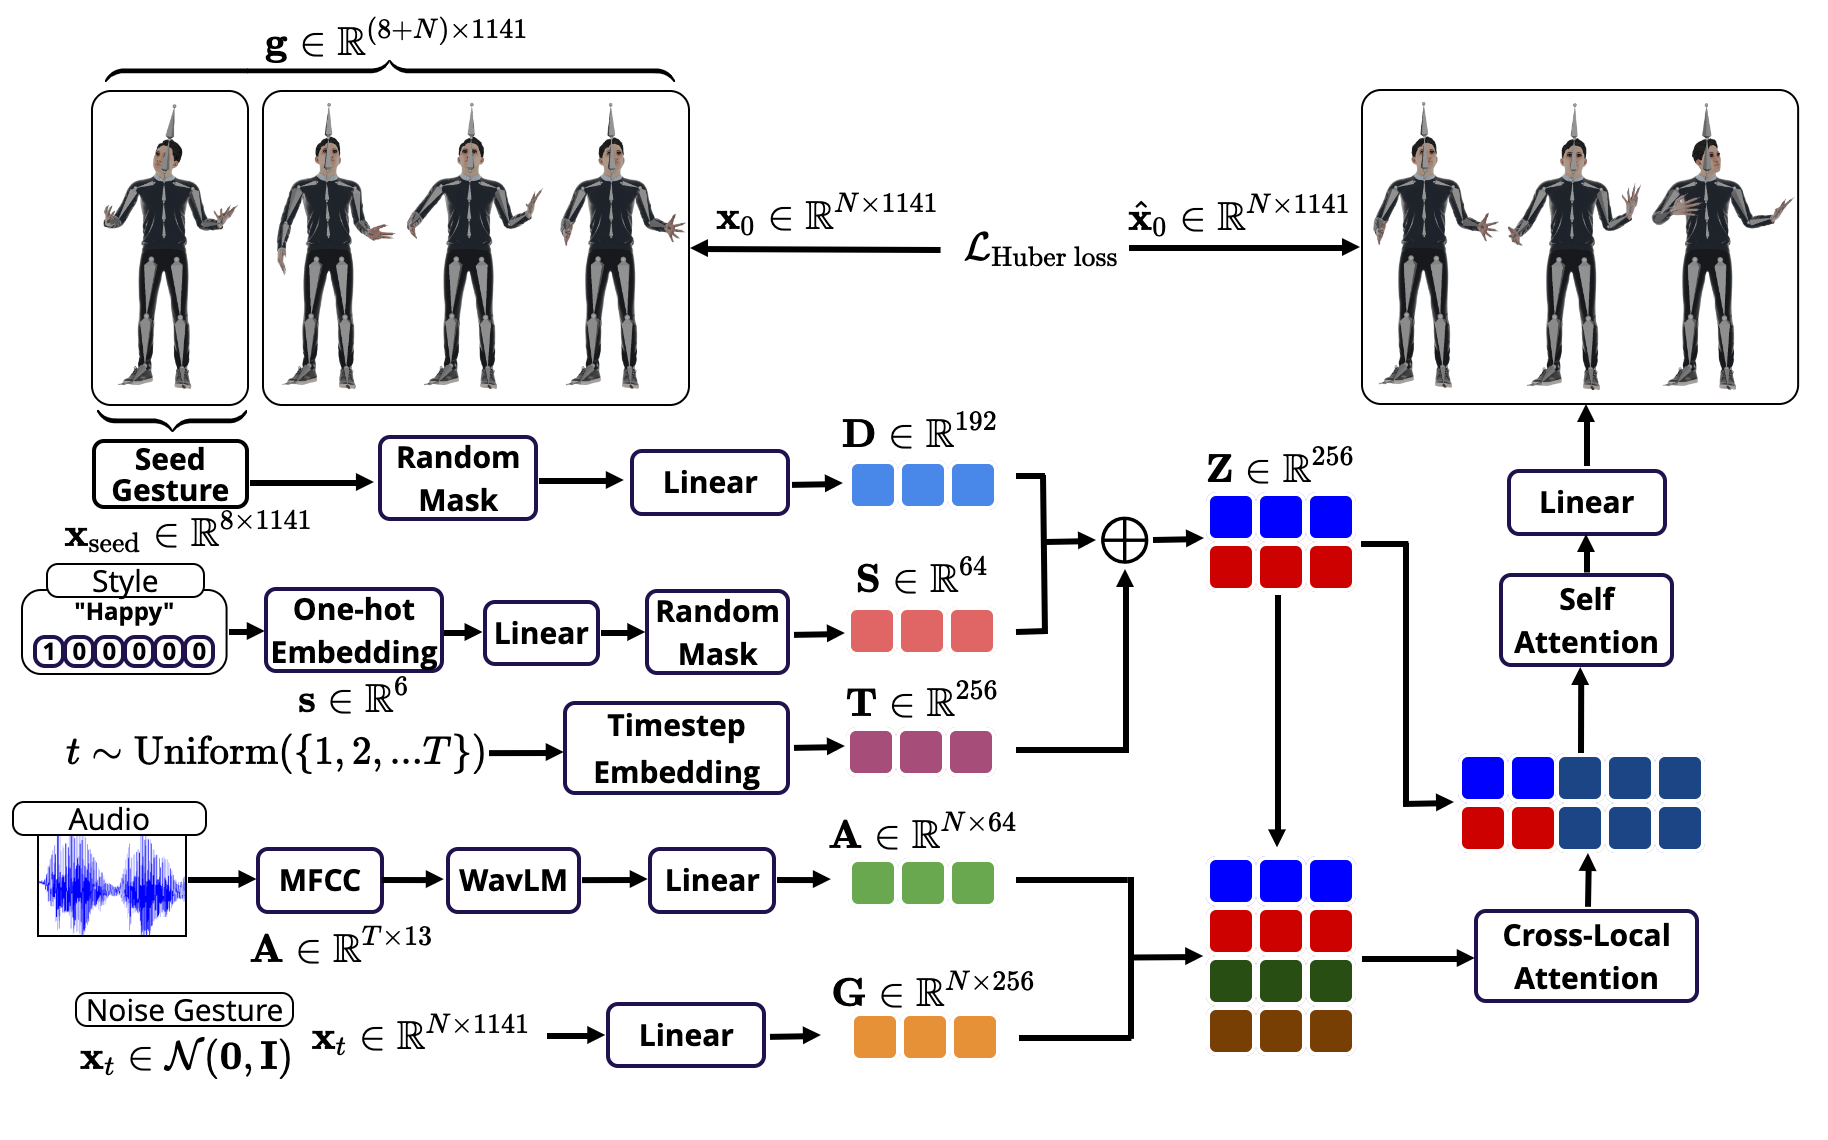
\includegraphics[width=\linewidth]{images/architecture_diffusion}
	\caption{Kiến trúc OHGesture}
	\label{fig:architecturediffusion}
\end{figure}


% Ý tưởng của chúng tôi là tạo ra các cử chỉ bằng một mô hình diffusion \cite{ho2020denoising} bằng cách học cách dần dần Denoise từ nhiễu hoàn toàn. Như được thể hiện trong Hình 2, mô hình diffusion bao gồm hai phần: quá trình tiến lùi (quá trình diffusion)  và quá trình ngược lại (quá trình Denoise).

%\subsection{Quá Trình Gây Nhiễu (Diffusion)}
%
%Quá trình diffusion $q$ được mô hình hóa như là một quá trình Markov với đầu vào lần lượt được thêm nhiễu, và sau đó mô hình lần lượt từng bước học để có thể tái tạo lại cử chỉ ban đầu.
%Trong bài toán sinh cử chỉ, đầu vào là các điểm trên tọa độ 3D, gọi là keypoint $x$, với $x_{0} \sim q\left(x_{0}\right)$ và $q\left(x_{0}\right)$ là phân phối của dữ liệu thực tế.
%Trong đó mỗi bước phương sai được thay đổi theo hệ số $\beta_{1}, \beta_{2}, \ldots, \beta_{T}$ $\left(0<\beta_{1}<\beta_{2}<\cdots<\beta_{T}<1, T\right)$, chúng tôi thêm nhiễu Gaussian
%
%\begin{equation} \label{eq:gaussian}
%q\left(x_{t} \mid x_{t-1}\right)=\mathcal{N}\left(x_{t} ; \sqrt{1-\beta_{t}} x_{t-1}, \beta_{t} \mathbf{I}\right)
%\end{equation}
%
%vào cử chỉ tại mỗi thời điểm $t$ lần lượt, và sau khi nhiễu Guassian được thêm vào đến bước $T$ đủ lớn, đến khi kết quả trở nên nhiễu hoàn toàn và không thể phân biệt được với kết quả ban đầu.

%\subsection{Quá Trình Khử Nhiễu (Denoise)}
%
%Quá trình Denoise $p_{\theta}$ là quá trình học tham số $\theta$ thông qua một mạng neural. Giả sử quá trình Denoise cũng tuân theo phân phối Gaussian, tức là nhiễu $x_{t}$ tại thời điểm $t$ được sử dụng để học $\mu_{\theta}, \Sigma_{\theta}$, sau đó
%
%\begin{equation} \label{eq:diffusion}
%p_{\theta}\left(x_{t-1} \mid x_{t}\right)=\mathcal{N}\left(x_{t-1} ; \mu_{\theta}\left(x_{t}, t\right), \Sigma_{\theta}\left(x_{t}, t\right)\right)
%\end{equation}
%
%Để thuận tiện cho việc tính toán, ta cho $\alpha_{t}=1-\beta_{t}$ và viết gọn lại $\bar{\alpha}_{t}=\prod_{i=1}^{T} \alpha_{i}$. Sau đó, cử chỉ nhiễu $x_{t}$ tại thời điểm $t$ có thể được viết lại như sau:
%
%\begin{equation} \label{eq:denoisevariance}
%q\left(x_{t} \mid x_{0}\right)=\mathcal{N}\left(x_{t} ; \sqrt{\bar{\alpha}_{t}} x_{0},\left(1-\bar{\alpha}_{t}\right) \mathbf{I}\right)
%\end{equation}
%
%Mô hình học bằng cách tối ưu hóa bằng cách giảm thiểu sự khác biệt giữa nhiễu thực sự $\epsilon$ và nhiễu được dự đoán $\epsilon_{\theta}\left(x_{t}, t\right)$ \cite{ho2020denoising}. Khi lấy mẫu, chúng ta có thể học giá trị trung bình $\mu_{\theta}\left(x_{t}, t\right)=\frac{1}{\sqrt{\alpha_{t}}}\left(x_{t}-\frac{\beta_{t}}{\sqrt{1-\bar{\alpha}_{t}}} \epsilon_{\theta}\left(x_{t}, t\right)\right)$ với phương sai cố định.

\subsection{Sinh cử chỉ với điều kiện}

Mục tiêu của chúng tôi là tổng hợp một cử chỉ con người $x^{1: N}$ có độ dài $N$ dựa trên điều kiện $c$. Trong mô hình OHGesture, tương tự như các phương pháp \cite{ramesh2022hierarchical} \cite{tevet2022human}, chúng tôi dự đoán dự liệu thật thay vì dự đoán nhiễu $\epsilon_{\theta}\left(x_{t}, t\right)$ như \cite{ho2020denoising}. Quá trình khử nhiễu (Denoise) tái tạo dữ liệu gốc $x_{0}$ dựa trên nhiễu đầu vào $x_{t}$, bước làm nhiễu $t$ và điều kiện $c$

\begin{equation} \label{eq:condition}
\hat{x}_{0}=\text { Denoise }\left(x_{t}, t, c\right)
\end{equation}

Sau đó, hàm khử nhiễu có thể được huấn luyện bằng cách tối ưu hóa hàm Huber loss \cite{huber1992robust} giữa các cử chỉ dự đoán $\hat{x}_{0}$ và các cử chỉ thực tế $x_{0}$ trên các tập huấn luyện:

\begin{equation} \label{eq:huberloss}
\mathcal{L}=E_{x_{0} \sim q\left(x_{0} \mid c\right), t \sim[1, T]}\left[\operatorname{HuberLoss}\left(x_{0}-\hat{x}_{0}\right)\right]
\end{equation}

\section{Áp dụng cơ chế Attention cho bài toán sinh cử chỉ}

\subsection{Hàm xử lý đặc trưng của quá trình khử nhiễu}

Như kiến trúc \textbf{OHGesture} trình bày trong hình \autoref{fig:architecturediffusion}, cử chỉ được tạo ra dựa trên bước làm nhiễu $t$, cử chỉ nhiễu $x_{t}$ và điều kiện $c$ (bao gồm âm thanh $a$, cảm xúc $s$ và cử chỉ khởi tạo $d$ ). Đối với mỗi đặc trưng, quá trình sinh cử chỉ được xử lý như sau:


\subsection{Cơ chế Attention trong hàm khử nhiễu}

Chúng tôi thực hiện việc khử nhiễu với kiến trúc dựa trên cơ chế attention. Để tính được tương quan của các đặc trưng xa, chúng tôi sẽ học để biểu diễn được các ngữ cảnh cực bộ (local context) theo \cite{rae2020transformers}.

Đầu tiên cử chỉ khởi tạo $\mathbf{D}$ và vector cảm xúc $\mathbf{S}$ được ghép lại với nhau để tạo thành một vectơ có kích thước 256, sau đó thêm vector làm nhiễu $\mathbf{T}$ để tạo thành vector $\mathbf{Z}$. 
Sau đó, vectơ $\mathbf{Z}$ và các bản sao của nó được ghép thành một chuỗi vector đặc trưng để khớp với dòng thời gian của âm thanh và đặc trưng cử chỉ, sau đó ghép với âm thanh $\mathbf{A}$ và cử chỉ $\mathbf{G}$ để làm đầu vào cho lớp local attention (chú ý cục bộ). 
Phương pháp sinh cử chỉ song hành với âm thanh của chúng tôi sử dụng lớp Local Attention được lấy ý tưởng từ phương pháp Routing Transformer \cite{roy2021efficient}, mà cho thấy rằng local attention quan trọng trong việc xây dựng biểu diễn trung gian, như được thể hiện trong Hình 3(c).

Sau đó, chúng tôi nối đầu ra của lớp local attention với $\mathbf{Z}$ và đưa vào lớp self-attention, như được thể hiện trong \autoref{fig:architecturediffusion}. Cơ chế self-attention tương tự như trình mã hóa (encoding) của Transformer \cite{vaswani2017attention}, giúp tính toán được mối liên hệ giữa các chuỗi dữ liệu với công tức sau:


\begin{equation} \label{eq:attention}
\operatorname{Attention}(\mathbf{Q}, \mathbf{K}, \mathbf{V}, \mathbf{M})=\operatorname{softmax}\left(\frac{\mathbf{Q} \mathbf{K}^{T}+\mathbf{M}}{\sqrt{C}}\right) \mathbf{V}
\end{equation}

trong đó $\mathbf{Q}, \mathbf{K}, \mathbf{V}$ là vector query, key và value từ dữ liệu đầu vào và $\mathbf{M}$ là mặt nạ (mask) giúp xác định loại của cơ chế attention, bao gồm \textit{full self-attention}, \textit{sliding window attention} và \textit{cross-local attention}. Để yếu tố thời gian không ảnh hưởng nhiều đến kết quả sinh cử chỉ, chúng tôi sử dụng cơ chế mã hóa vị trí tương đối (Relative Position Encoding - RPE) được trình bày trong phương pháp Reformer \cite{kitaev2020reformer}. Cuối cùng, đầu ra của self-attention được ánh xạ lại cùng kích thước như $x_{0}$ sau một lớp biến đổi tuyến tính.

\begin{figure*}[ht]
\begin{minipage}[b]{0.25\textwidth}
\centering
    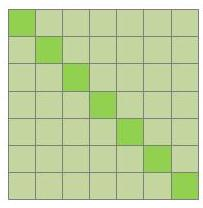
\includegraphics[width=\textwidth]{images/attention_full.jpg}
    \caption*{(a) full self-attention}
\end{minipage}
\hfill
\begin{minipage}[b]{0.25\textwidth}
\centering
    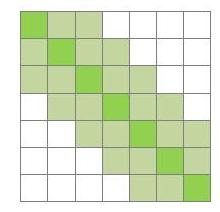
\includegraphics[width=\textwidth]{images/attention_sidewindow.jpg}
    \caption*{(b) sliding window attention}
\end{minipage}
\hfill
\begin{minipage}[b]{0.25\textwidth}
\centering
    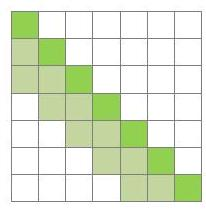
\includegraphics[width=\textwidth]{images/cross_attention.jpg}
    \caption*{(c) cross-local attention}
\end{minipage}
% \label{fig:type_attention}
\caption[Các loại attention khác nhau (full self-attention, sliding window attention, cross-local attention)]{Các loại attention khác nhau được sử dụng trong các thí nghiệm của chúng tôi, trong đó (a) và (c) là cơ chế attention được sử dụng trong mô hình của chúng tôi và (b) là một mẫu được sử dụng để đánh giá trong thực nghiệm. Mỗi dòng tương ứng với input và mỗi cột tương ứng với output của mô hình}
\end{figure*}

% Phần 4.3. Các hàng đại diện cho các đầu ra và các cột đại diện cho đầu vào. Các hình vuông màu sáng tô màu cho các phần tử liên quan đến mỗi dòng đầu ra.


Các cơ chế attention khác nhau có thể được tạo ra bằng cách điều chỉnh lớp mask tương ứng $\mathbf{M}$, 
tương tự như phương pháp Longformer \cite{beltagy2020longformer} chúng tôi cũng thử nghiệm cơ chế \textit{sliding window attention}.

\subsection{Phương pháp sample cử chỉ}

Để có thể sinh cử chỉ với chiều dài tùy ý, chúng tôi cắt chuỗi ban đầu thành các đoạn ngắn có chiều dài $N$. Trong quá trình huấn luyện, cử chỉ khởi tạo đầu tiên có thể được tạo ra bằng cách lấy ngẫu nhiên cử chỉ từ tập dữ liệu hoặc từ lấy trung bình từ đoạn cắt được. Cụ thể ở đây, sẽ lấy góc quay trung bình trong các đoạn đã cắt được. Tiếp theo chúng ta chỉ việc lấy lần lượt các frame đã sinh ra và chọn $8$ frame cuối cùng làm cử chỉ khởi tạo ở lượt tiếp theo. Đối với mỗi đoạn đã cắt ra, cử chỉ $x_{t}$ lần lượt sẽ được áp dụng hàm khử nhiều $\hat{x}_{0} = Denoise \left(x_{t}, t, c\right)$ cho đến khi được  $x_{t-1}$, và $x_{t-1}$ sẽ tiếp tục được làm khử nhiễu cho đến bước khử nhiễu $t=T$ sẽ đạt được $x_{0}$ như kiến trúc trong phần \autoref{fig:architecturediffusion}.


% chúng tôi , trong mỗi bước làm nhiễu $t$, chúng tôi dự đoán cử chỉ sạch  $=$  $\left(x_{t}, t, c\right)$, và thêm nhiễu vào bước làm nhiễu $x_{t-1}$ sử dụng Phương trình (1) với quá trình trải đều. Quá trình này được lặp lại từ $t=T$ cho đến khi đạt được $x_{0}$ (Hình 2 dưới cùng).

\section{Điều khiển cảm xúc trong bài toán sinh cử chỉ}

\begin{figure}[htbp]
    \centering
    \begin{subfigure}[b]{0.3\textwidth}
         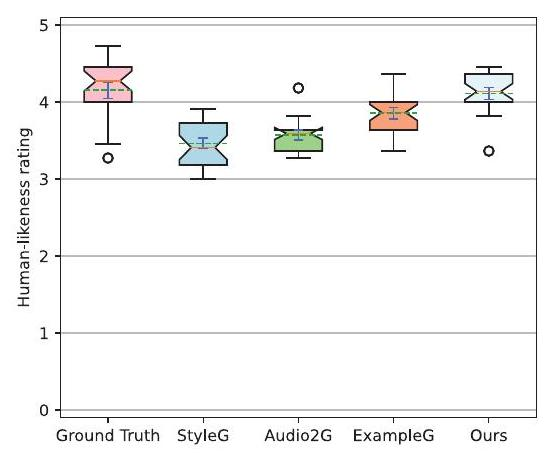
\includegraphics[width=\textwidth]{images/humanlike_score.jpg}
        \caption*{(a) Biểu đồ hộp của đánh giá về tính giống với con người}
    \end{subfigure}
    \hfill
    \begin{subfigure}[b]{0.3\textwidth}
        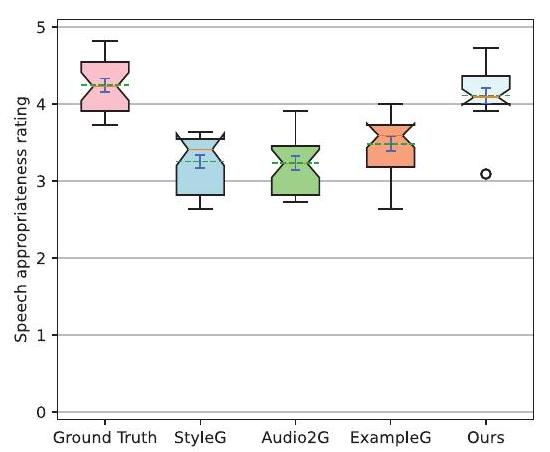
\includegraphics[width=\textwidth]{images/speech_score.jpg}
         \caption*{(b) Biểu đồ hộp của đánh giá về tính phù hợp giữa cử chỉ và âm thanh.}
    \end{subfigure}
    \hfill
    \begin{subfigure}[b]{0.3\textwidth}
        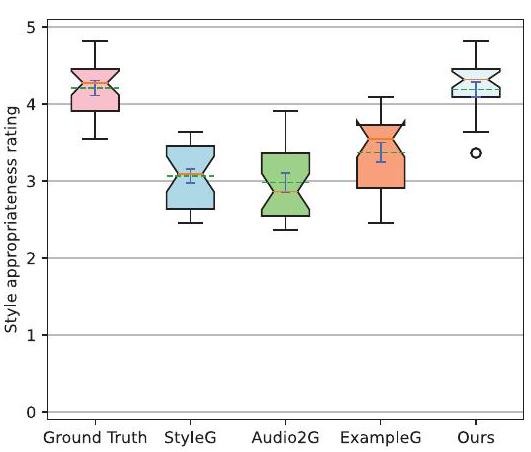
\includegraphics[width=\textwidth]{images/style_score.jpg}
        \caption*{(c) Biểu đồ hộp của đánh giá về tính phù hợp giữa cử chỉ và cảm xúc}
    \end{subfigure}
    \caption[Biểu đồ hộp mô tả kết quả so sánh MOS]{Biểu đồ hộp mô tả kết quả so sánh MOS cho các mô hình khác nhau trong các chiều khác nhau. Hộp mở rộng từ phân vị thứ nhất thấp nhất (Q1) đến phân vị thứ ba lớn nhất (Q3) của dữ liệu. Đường đỏ chỉ là giữa. Các khe nhỏ biểu thị khoảng tin cậy $95\%$ (CI) xung quanh giữa. Khi CI nhỏ hơn Q1 hoặc lớn hơn Q3, khe mở rộng ra khỏi hộp, tạo ra một hình dáng "lật" độc đáo. Chúng tôi cũng đã đánh dấu giá trị trung bình và khoảng tin cậy $95\%$ của nó trong hình với đường nét đứt màu xanh lá cây và đường dọc màu xanh lam, tương ứng.}
    \label{fig:3col}
\end{figure}


Ở các bước trên mô hình đã có thể học được cách sinh cử chỉ, nhưng để mô hình có thể học được các cảm xúc ở các tình huống khác nhau sẽ được giải quyết bằng cách tham số hóa và lần lượt thay đổi từng cảm xúc để sao cho khi thay đổi cảm xúc thì kết quả dự đoán phải có cảm xúc tương ứng.
Tham số để điều khiển ở đây là $c$, việc điều khiển ở đây không chỉ có thể là âm thanh $a$ mà còn là cảm xúc $s$ hoặc cử chỉ khởi tạo $d$, v.v. Chúng tôi tham khảo phương pháp của \cite{ho2022classifier}, \cite{tevet2022human}, bằng cách thêm một lớp mặt nạ ngẫu nhiên (random mask) trên các vector đặc trưng của cử chỉ khởi tạo $d$ và cảm xúc $s$ vào mô hình như hình minh họa \autoref{fig:architecturediffusion} để giúp kiểm soát chính xác việc mô hình có thể học được các đặc trưng ở các điều kiện khác nhau. Khi đó, mô hình chỉ việc thay đổi nhãn tương ứng với lớp mask đã lấy ngẫu nhiên để mô hình có thể tối ưu theo các điều kiện khác nhau. Khi đó hàm khử nhiễu $\text{Denoise} \left(x_{t}, t, c_{1}\right), c_{1}=[d, s, a]$ và hàm khử nhiễu mà không có điều kiện $\text{Denoise} \left(x_{t}, t, c_{2}\right), c_{2}=[\varnothing, \varnothing, a]$ sẽ được tối ưu trong quá trình huấn luyện, theo công thức

\begin{equation} \label{eq:denoise}
\hat{x}_{0 \gamma, c_{1}, c_{2}}=\gamma \text{Denoise} \left(x_{t}, t, c_{1}\right)+(1-\gamma) \text{Denoise} \left(x_{t}, t, c_{2}\right)
\end{equation}


Trong thực tế, hàm Denoise học cả phân phối có điều kiện và không có điều kiện bằng cách ngẫu nhiên phần mask $10 \%$ của các mẫu bằng các mask theo phân phối Bernoulli. Sau đó, đối với kiểu $s$ trong điều kiện, chúng ta có thể tạo ra cử chỉ được kiểm soát kiểu khi lấy mẫu bằng cách nội suy hoặc thậm chí là dự đoán hai biến thể bằng cách sử dụng $\gamma$, như $c_{1}=\left[d, s_{1}, a\right], c_{2}=\left[d, s_{2}, a\right]$

% \begin{figure*}[ht]
% \begin{minipage}[b]{0.3\textwidth}
% \centering
%     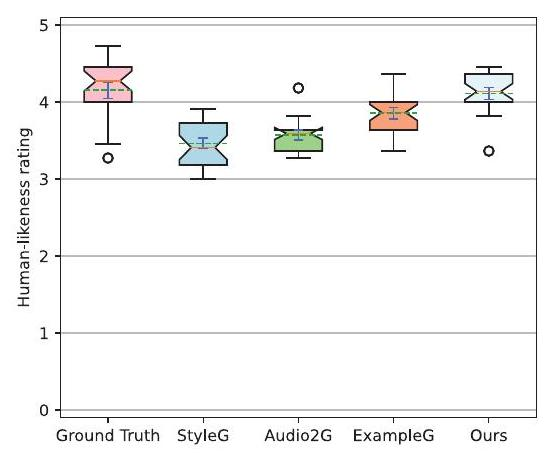
\includegraphics[width=\textwidth]{images/humanlike_score.jpg}
%     \caption*{(a) Biểu đồ hộp của đánh giá về tính giống với con người}
% \end{minipage}
% \hfill
% \begin{minipage}[b]{0.3\textwidth}
% \centering
%     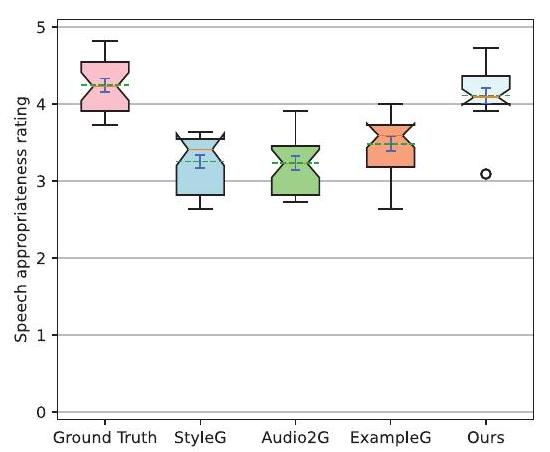
\includegraphics[width=\textwidth]{images/speech_score.jpg}
%     \caption*{(b) Biểu đồ hộp của đánh giá về tính phù hợp giữa cử chỉ và âm thanh.}
% \end{minipage}
% \hfill
% \begin{minipage}[b]{0.3\textwidth}
% \centering
%     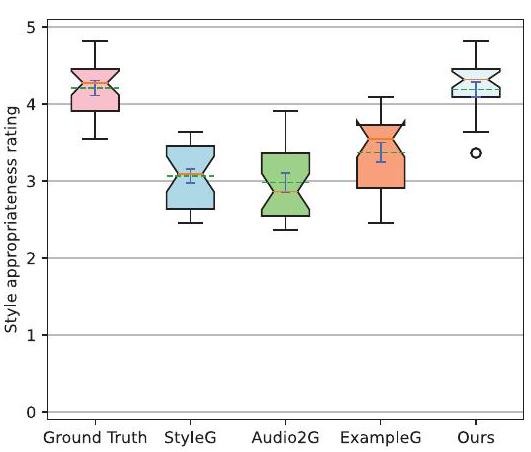
\includegraphics[width=\textwidth]{images/style_score.jpg}
%     \caption*{(c) Biểu đồ hộp của đánh giá về tính phù hợp giữa cử chỉ và cảm xúc}
% \end{minipage}
% \label{fig:gesture_score}
% \caption{Biểu đồ hộp mô tả kết quả so sánh MOS cho các mô hình khác nhau trong các chiều khác nhau. Hộp mở rộng từ phân vị thứ nhất thấp nhất (Q1) đến phân vị thứ ba lớn nhất (Q3) của dữ liệu. Đường đỏ chỉ là giữa. Các khe nhỏ biểu thị khoảng tin cậy $95\%$ (CI) xung quanh giữa. Khi CI nhỏ hơn Q1 hoặc lớn hơn Q3, khe mở rộng ra khỏi hộp, tạo ra một hình dáng "lật" độc đáo. Chúng tôi cũng đã đánh dấu giá trị trung bình và khoảng tin cậy $95\%$ của nó trong hình với đường nét đứt màu xanh lá cây và đường dọc màu xanh lam, tương ứng.}
% \end{figure*}


% Hình 4: Biểu đồ hộp thể hiện kết quả so sánh của MOS cho các mô hình khác nhau trong các chiều không gian khác nhau. Hộp mở rộng từ phần tư dưới thứ nhất (Q1) đến phần tư lớn thứ ba (Q3) của dữ liệu. Đường đỏ chỉ ra trung vị. Các rãnh biểu thị khoảng tin cậy $95 \%$ (CI) xung quanh trung vị. Khi CI ít hơn Q1 hoặc lớn hơn Q3, rãnh mở rộng ra ngoài hộp, tạo cho nó một diện mạo "lật" độc đáo. Chúng tôi cũng đã đánh dấu giá trị trung bình và CI $95\%$ của nó trong hình với một đường kẻ xanh lá cây đứt và một đường kẻ đứt màu xanh dương, tương ứng.

% \begin{equation}
% \left[\mathbf{r}_p, \mathbf{r}_r, \dot{\mathbf{r}}_p, \dot{\mathbf{r}}_r, \rho_p, \rho_r, \dot{\rho}_p, \dot{\rho}_r, g_d\right]
% \end{equation}


% Mô hình OHGesture được dựa trên mô hình QPGesture \cite{yang2023qpgesture} với nền tảng chính của phương pháp dựa trên mô hình VQ-VAE là mã hóa (encode) và giải mã (decode) dữ liệu hay nói cách khác chúng ta sẽ biểu diễn toàn bộ dữ liệu ở chiều dữ liệu thấp hơn và sau đó biểu diễn ngược trở lại kích thước ban đầu. Dữ liệu được biểu diễn thành các vùng trong không gian, với mỗi vùng có một đại diện tương ứng. Từ các địa diện ta có thể mã hóa ngược trở lại để chọn ra các ứng viên cử chỉ theo ngữ nghĩa (dữ liệu văn bản) hoặc nhịp điệu lời nói (dữ liệu âm thanh).
% Dựa trên hai cử chỉ ứng viên (gesture candidate), ta trích xuất ra pha dựa trên vận tốc xoay của các các khớp khi di chuyển và dựa trên pha hiện tại của cử chỉ khởi tạo, ta sẽ chọn được cử chỉ có pha gần nhât hay phù hợp nhất để chọn ra chuỗi cử chỉ cuối cùng.

% Cụ thể quá trình huấn luyện của mô hình bao gồm các quá trình như sau: Lượng tử hóa (Quantization), Ghép các chuyển động cử chỉ (Motion Matching), Điều hướng dựa theo pha của cử chỉ (Phrase Guided).

% Kiến trúc mô hình được trình bày minh họa trong hình \autoref{fig:architecturediffusion}.








% \subsection{Lượng tử hóa (Quantization)}
% % Learning a discrete latent space representation

% Lượng tử hóa là việc học để biểu diễn dữ liệu trong không gian rời rạc (discrete latent space representation). Ta sẽ biểu diễn dữ liệu lên không gian tiềm ần (latent space).
% Mục tiêu của việc lượng tử hóa là biểu diễn dữ liệu dưới số chiều thấp hơn hay chấm điểm/đánh giá dựa trên các đặc trưng của dữ liệu, từ đó dùng các điểm đã đánh giá để so sánh với nhau. Sau khi so sánh đánh giá, ta chọn được một ứng viên tốt nhất, từ ứng viên tốt nhất ta sẽ học để giải mã (decode) ngược trở lại dữ liệu ban đầu.

% Dữ liệu đầu vào được lượng tử hóa bao gồm âm thanh, cử chỉ và văn bản. Trong bài toán sinh cử chỉ, chúng tôi chỉ tập trung vào việc xử lý dữ liệu dựa trên cử chỉ nên đôi với dữ liệu văn bản và âm thanh, ta chỉ sử dụng lại các mô hình pre-train có sẵn. Với âm thanh chúng tôi sử dụng mô hình VQ-Wave2Vec \cite{baevski2019vq} để biểu diễn các dữ liệu âm thanh thành các latent vector. Hàm lượng tử hóa âm thanh là hàm $f_{quant\_audio} : \mathbf{A} \mapsto \mathbf{Z_{audio}}$ trong đó $\textbf{A}$ là các chuỗi các âm thanh sẽ được mã hóa lên vector lantent $\textbf{Z}$. Với $\textbf{Z_{audio}} \in \mathcal{Z}_a$.

% Đối với văn bản, chúng tôi sử dụng mô hình Sentene BERT \cite{reimers2019sentence} để biểu diễn các dữ liệu văn bản thành các vector tiềm ẩn. Hàm để nhúng các dữ liệu văn bản thành các vector là hàm $f_{embedding\_text} : \mathbf{T} \mapsto \mathbf{Z_{text}}$.

% Với cử chỉ, mô hình dựa trên kiến trúc của mô hình VQ-VAE. Hàm lượng tử hóa cử chỉ là hàm $f_{quant\_gesture} : \mathbf{G} \mapsto \mathbf{Z_{gesture}}$ với $\textbf{G}$ là các vector trong codebook $\mathcal{Z_g}$

% % Sau đó dựa trên các điểm dữ liệu trước đó để tìm được đại diện phù hợp trong các vùng.
% % Dựa trên chuỗi các dữ liệu đại diện ta có thể tìm được chuỗi các pha của cử chỉ và từ đó chọn ra điểm dữ liệu cuối cùng dựa trên pha của văn bản hoặc âm thanh.

% \subsubsection{Hàm lượng tử hóa cử chỉ (Gesture Quantization)}

% Trong $f_{quant\_gesture}$ các điểm dữ liệu được phân tách và gom nhóm thành các vùng khác nhau trong không gian, với một đại diện để biểu diễn cho mỗi vùng được gọi là \textit{code} là một vector $\textbf{z} \in \mathbb{R}$. Tập các vector đại diện cho các vùng được gọi là \textit{codebook} $\mathbf{Z} \in \mathbb{R}^{D_g \times C}$ là một từ điển được biểu thị dưới dạng một ma trận bao gồm tập nhiều codebook, với mỗi code $\textbf{z} \in \mathbb{R}^C$ và $D_g$ là số lượng phần tử của codebook.

% $$
% f_{encoder} : \mathbf{X} \mapsto \mathbf{Z} \quad \quad
% f_{quantize} : \mathbf{Z} \mapsto \hat{\mathbf{Z}} \quad \quad
% f_{decoder} : \hat{\mathbf{Z}} \mapsto \mathbf{C}
% $$

% $$
% \mathcal{L}=\mathcal{L}_{\text {recontruct }}\left(\mathbf{c}, \mathbf{x}\right)+\left\|\operatorname{sg}[\mathbf{z}]-\mathbf{z}_{\mathbf{q}}\right\| +\beta\left\|\mathbf{z}-\operatorname{sg}\left[\mathbf{z}_{\mathbf{q}}\right]\right\|
% $$

% Loss function:
% $$
% \mathcal{L}_{\text {gesture }\left(E_{g}, D_{g}, \mathcal{Z}_{g}\right)}=\mathcal{L}_{\text {rec }}\left(\hat{\mathbf{G}}_{1}, \mathbf{G}\right)+\left\|\operatorname{sg}[\mathbf{g}]-\mathbf{g}_{\mathbf{q}}\right\| +\beta\left\|\mathbf{g}-\operatorname{sg}\left[\mathbf{g}_{\mathbf{q}}\right]\right\|
% $$

% Loss recontruction:

% $$
% \mathcal{L}_{r e c}\left(\hat{\mathbf{G}}_{1}, \mathbf{G}_{1}\right)=\left\|\hat{\mathbf{G}_{1}}-\mathbf{G}_{1}\right\|_{1}+\alpha_{1}\left\|\hat{\mathbf{G}}_{1}{ }^{\prime}-\mathbf{G}_{1}^{\prime}\right\|_{1} +\alpha_{2}\left\|\hat{\mathbf{G}}_{1}{ }^{\prime \prime}-\mathbf{G}_{1}^{\prime \prime}\right\|_{1}
% $$

% \subsubsection{Quantization Audio}


% $
% \mathbf{g}_{\mathbf{q}, i}=\mathcal{Q_g}(\mathbf{g})=\arg \min _{\mathbf{z}_{j} \in \mathcal{Z}_{g}}\left\|\mathbf{g}_{i}-\mathbf{z}_{j}\right\|
% $

% $
% \hat{\mathbf{G}}_{1}=\mathcal{D}_{g}\left(\mathbf{g}_{\mathbf{q}}\right)=\mathcal{D_g}\left(\mathcal{Q_g}\left(\mathcal{E_g}(\mathbf{G})\right)\right)
% $

% $
% \mathcal{L}=\sum_{k=1}^K \mathcal{L}_k^{\text {wav2vec }}+\left(\|\operatorname{sg}(\mathbf{z})-\hat{\mathbf{z}}\|^2+\gamma\|\mathbf{z}-\operatorname{sg}(\hat{\mathbf{z}})\|^2\right)
% $

% $
% \mathcal{L}_k^{\text {wav2vec }}=-\sum_{i=1}^{T-k}\left(\log \sigma\left(\mathbf{z}_{i+k}^{\top} h_k\left(\mathbf{c}_i\right)\right)+\underset{\tilde{\mathbf{z}} \sim p_n}{\mathbb{E}}\left[\log \sigma\left(-\tilde{\mathbf{z}}^{\top} h_k\left(\mathbf{c}_i\right)\right)\right]\right)
% $


% \section{Motion Matching}
% $
% \hat{\mathbf{C}}_{a}=\left\{\hat{\mathbf{C}}_{a}^{0}, \hat{\mathbf{C}}_{a}^{1}, \ldots, \hat{\mathbf{C}}_{a}^{C_{b}}\right\}
% $

% $
% \hat{\mathbf{C}}_{g}=\left\{\hat{\mathbf{C}}_{g}^{0}, \hat{\mathbf{C}}_{g}^{1}, \ldots, \hat{\mathbf{C}}_{g}^{C_{b}}\right\}
% $

% $
% \hat{\mathbf{C}}_{t}=\left\{\hat{\mathbf{C}}_{t}^{0}, \hat{\mathbf{C}}_{t}^{1}, \ldots, \hat{\mathbf{C}}_{t}^{C_{b}}\right\}
% $



% \subsection{Phrase Guidance}

% \begin{figure}
%     \centering
%     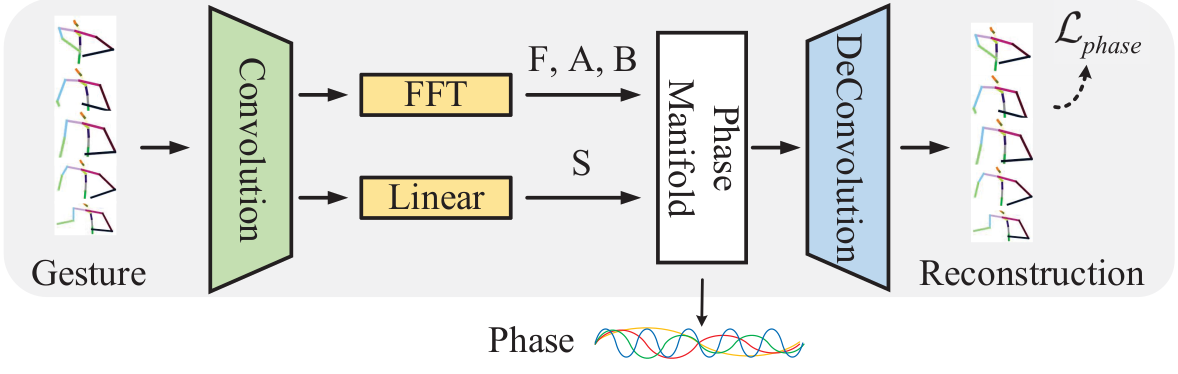
\includegraphics[width=\linewidth]{images/phrase_guidance.png}
%     \caption{Phrase Guidance}
%     \label{fig:PhraseGuidance}
% \end{figure}


% Hàm pha

% $$
% f(\mathcal{T} ; \mathbf{A}, \mathbf{F}, \mathbf{B}, \mathbf{S})=\mathbf{A} \cdot \sin (2 \pi \cdot(\mathbf{F} \cdot \mathcal{T}-\mathrm{S}))+\mathbf{B}
% $$

% Hàm encoder

% $$
% \mathbf{L}=E_{p}(\mathbf{G_{ \text{rotation\_velocity} }})
% $$

% Hàm fourier 
% $$
% \mathbf{c}=F F T(\mathbf{L});\ \ \mathbf{c} \in \mathbb{C}^{M \times K+1}, K=\left|\frac{T}{2}\right|
% $$

% $$
% \mathbf{f}=(0,1 / N, 2 / N, \ldots, K / N)
% $$

% $$
% \mathbf{A}_{i}=\sqrt{\frac{2}{T} \sum_{j=1}^{K} \mathbf{p}_{i, j}}
% $$

% $$
% \quad \mathbf{F}_{i}=\frac{\sum_{j=1}^{K}\left(\mathbf{f}_{j} \cdot \mathbf{p}_{i, j}\right)}{\sum_{j=1}^{K} \mathbf{p}_{i, j}}
% $$


% $$
% \quad \mathbf{B}_{i}=\frac{\mathbf{c}_{i, 0}}{T},
% $$

% Phrase shift
% $$
% \left(s_{x}, s_{y}\right)=F C\left(\mathbf{L}_{i}\right), \quad \mathbf{S}_{i}=\operatorname{atan} 2\left(s_{y}, s_{x}\right)
% $$

% $$
% \mathcal{T}=\left[-\frac{t_{1}-t_{0}}{2},-\frac{t_{1}-t_{0}}{2}+\frac{t_{1}-t_{0}}{N-1}, \ldots, \frac{t_{1}-t_{0}}{2}\right]
% $$


% $$
% \hat{\mathbf{L}}=f(\mathcal{T} ; \mathbf{A}, \mathbf{F}, \mathbf{B}, \mathbf{S})=\mathbf{A} \cdot \sin (2 \pi \cdot(\mathbf{F} \cdot \mathcal{T}-\mathrm{S}))+\mathbf{B}
% $$

% $$
% \hat{\mathbf{G}}_{2}=h(\hat{\mathbf{L}})
% $$

% $$
% \mathcal{P}_{2 i-1}^{(t)}=\mathrm{A}_{i}^{(t)} \cdot \sin \left(2 \pi \cdot \mathrm{S}_{i}^{(t)}\right), \mathcal{P}_{2 i}^{(t)}=\mathrm{A}_{i}^{(t)} \cdot \cos \left(2 \pi \cdot \mathrm{S}_{i}^{(t)}\right)
% $$

% $$
% \mathcal{P} \in \mathbb{R}^{2\ M}
% $$

% $$\mathcal{L}_{\text {phase }}=\mathcal{L}_{\text {phase-recon }}\left(\mathbf{G}, \hat{\mathbf{G}}_{\mathbf{2}}\right)$$




% $$
% \left(
% \left[
%     \hat{
%     \mathcal{P}}_o[-1]^{
%     \left[
%     \left(N_{
%     \text{strid}}-N_{
%     \text{phase}}
% \right):
% \right]}, 
% \mathcal{P}_{a, t}^{
%     \left[N_{
%     \text{strid}}:
% \right]}
% \right]
% \right. 
% , 
% \left.
% \left[
%     \hat{
%     \mathcal{P}}_o[-1]^{
%     \left[-N_{
%     \text{strid}}:
% \right]}, 
% \mathcal{P}_{a, t}^{
%     \left[
%     \left(N_{
%     \text{phase}}-N_{
%     \text{strid}}
% \right):
% \right]}
% \right]
% \right)<
% $$


% $$
% \left(\left[    \hat{    \mathcal{P}}_o[-1]\left[    \left(N_{    \text{strid}}-N_{    \text{phase }}\right):\right], \mathcal{P}_{t, t}^{    \left[        N_{    \text{strid}}:\right]}\right]\right. ,    \left.\left[    \hat{    \mathcal{P}}_o[-1]^{    \left[        -N_{    \text{strid}}:\right]}, \mathcal{P}_{t, t}^{    \left[    \left(N_{    \text{phase }}-N_{    \text{strid}}\right):\right]}\right]\right)
% $$



% $$
% d\left(\operatorname{concat}\left[\hat{\mathcal{P}}_o[-1]\left[\left(N_{\text {strid }}-N_{\text {phase }}\right):\right], \mathcal{P}_{t, t}^{\left[N_{\text {strid }}:\right]}\right]\right. \text {, }   \left.\operatorname{concat}\left[\hat{\mathcal{P}}_o[-1]^{\left[-N_{\text {strid }}:\right]}, \mathcal{P}_{t, t}^{\left[\left(N_{\text {phase }}-N_{\text {strid }}\right):\right]}\right]\right)
% $$

% $$
% d\left(\operatorname{concat}\left[\hat{\mathcal{P}}_o[-1]^{\left[\left(N_{\text {strid }}-N_{\text {phase }}\right):\right]}, \mathcal{P}_{a, t}^{\left[N_{\text {strid }}:\right]}\right]\right. \text {, }   \left.\operatorname{concat}\left[\hat{\mathcal{P}}_o[-1]^{\left[-N_{\text {strid }}:\right]}, \mathcal{P}_{a, t}^{\left[\left(N_{\text {phase }}-N_{\text {strid }}\right):\right]}\right]\right)<
% $$


% $$
% \left[\mathcal{P}_{-1}^{\left[\left(N_{\text {strid }}-N_{\text {phase }}\right):\right]}, \mathcal{P}_{a / t}^{\left[N_{\text {strid }}:\right]}\right]
% $$

% $
% \left[\mathcal{P}_{-1}^{\left[-N_{\text {strid }}:\right]}, \mathcal{P}_{a / t}^{\left[\left(N_{\text {phase }}-N_{\text {strid }}\right):\right]}\right]
% $





% Kết quả thí nghiệm
\chapter{Thực nghiệm}
\label{Chapter4}

\section{So với các phương pháp hiện tại}
\label{sec:result}


Chúng tôi so sánh mô hình đề xuất của chúng tôi với StyleGestures \cite{alexanderson2020style}, Audio2Gestures \cite{li2021audio2gestures}, ExampleGestures \cite{ghorbani2023zeroeggs}. Hiện tại, các cử chỉ điều khiển bằng giọng nói thiếu các chỉ số mục tiêu phản ánh một cách nhất quán với nhận thức chủ quan của con người \cite{yoon2022genea}; \cite{kucherenko2021large}; \cite{alexanderson2022listen}, ngay cả với Fréchet gesture distance (FGD) \cite{yoon2022genea}, \cite{dabral2023mofusion}, do đó tất cả các điểm số thực nghiệm của chúng tôi được thực hiện thông qua đánh giá chủ quan của con người. Chúng tôi thực hiện đánh giá trên ba chiều. Hai chiều đầu tiên theo đánh giá trong GENEA \cite{yoon2022genea}, bao gồm đánh giá về độ giống con người và sự phù hợp giữa cử chỉ và giọng nói. Chiều thứ ba là sự phù hợp giữa cử chỉ và phong cách.

Nghiên cứu Người Dùng. Để hiểu về hiệu suất thị giác thực tế của phương pháp của chúng tôi, chúng tôi tiến hành một nghiên cứu người dùng giữa các trình tự cử chỉ được tạo ra bởi mỗi phương pháp được so sánh và dữ liệu chụp chuyển động thực. Độ dài của các đoạn clip được đánh giá dao động từ 11 đến 51 giây, với độ dài trung bình là 31.6 giây. Lưu ý rằng các cử chỉ clip được sử dụng cho đánh giá chủ quan ở đây dài hơn so với đánh giá GENEA \cite{yoon2022genea} (8-10 giây), vì một khoảng thời gian dài có thể tạo ra kết quả phù hợp rõ ràng và thuyết phục hơn \cite{yang2022reprgesture}. Người tham gia đánh giá trên một khoảng điểm từ 5 đến 1, với các nhãn (tốt nhất đến tệ nhất) là "tuyệt vời," "tốt," "công bằng," "kém," và "tệ." Thêm chi tiết về nghiên cứu người dùng được hiển thị trong tư liệu bổ sung.

Điểm số ý kiến trung bình (MOS) về độ giống con người, phù hợp giọng nói và phù hợp phong cách được báo cáo trong \autoref{fig:mosscore}. Nếu các góc của hai hộp không chồng lên nhau, chúng ta có thể coi đây là bằng chứng mạnh mẽ rằng các phân phối khác nhau đáng kể \cite{mcgill1978variations}. Phương pháp của chúng tôi vượt trội đáng kể so với các phương pháp tiên tiến được so sánh với độ giống con người, phù hợp giữa cử chỉ và giọng nói, cũng như phù hợp giữa cử chỉ và phong cách, và thậm chí tạo ra các kết quả cạnh tranh với dữ liệu thực tế ở cả ba chiều. Theo phản hồi từ người tham gia, cử chỉ được tạo ra bởi chúng tôi "có ý nghĩa ngữ nghĩa hơn", "tự nhiên hơn," và "phù hợp với phong cách," trong khi phương pháp của chúng tôi có "chuyển động trượt chân" so với Dữ liệu Thực. Tuy nhiên, đây là một vấn đề phổ biến đối với các hệ thống tạo ra chuyển động không dựa trên vật lý và có thể được giải quyết thông qua xử lý sau \cite{ghorbani2023zeroeggs}, \cite{luvizon2023scene}.

\begin{table}[t]
	\centering
	\caption{Impact of the positional encoding block.}
	\label{tab:pos_enc}
	
	\newcolumntype{Y}{>{\raggedleft\arraybackslash}X}
	\newcolumntype{Z}{>{\centering\arraybackslash}X}
%	\begin{tabularx}{\linewidth}{XlYY}
	
%		
	
%		\bottomrule
%		\begin{tabularx}{\linewidth}{XlYY}
%		\toprule
%		Dataset & System & FGD $\downarrow$ & PMB ($\%$) $\uparrow$ \\
%		\toprule
%		\multirow{2}{*}{TED} & Without positional encoding & 2.19 & 88.13 \\
%		& With positional encoding & $\bm{2.04}$ & $\bm{89.52}$ \\
%		\bottomrule
%		\end{tabularx}
 \begin{tabularx}{\linewidth}{XlYY}
	\toprule
	Dataset & System & FGD $\downarrow$ & PMB ($\%$) $\uparrow$ \\
	\toprule
	\multirow{2}{*}{TED} & encoding & 2.19 & 88.13 \\
	& With positional encoding & $2.04$ & $89.52$ \\
	\bottomrule
\end{tabularx}
%		\multirow{2}*{Trinity} & Without positional encoding & 11.15 & 89.98 \\
%				& With positional encoding & $\bm{10.78}$ & $\bm{91.36}$ \\
%\hline
%This is a long entry that will automatically adjust its width. & Short text & Another long entry that will also adjust its width. \\
%\hline
%More text & Another short entry & Yet another long entry to demonstrate text wrapping and width adjustment. \\
%\hline

\end{table}


% \section{Đánh Giá}
% \label{sec:experiments}
 % Khả năng Kiểm soát Cử chỉ

\subsection{Khả năng kiểm soát cử chỉ}
\label{subsec:stylecontrol}

Giả sử rằng âm thanh trung tính không ảnh hưởng đến phong cách của cử chỉ, chúng ta có thể tạo ra các cử chỉ được phong cách hóa với một bài nói trung tính bằng cách đặt $\gamma=1$ và $s$ trong \autoref{eq:denoise}. Chúng tôi chọn hai đoạn hội thoại trong tập kiểm thử với âm thanh trung tính để tạo ra sáu cử chỉ được phong cách hóa tương ứng. \autoref{fig:emotiondataset} minh họa cử chỉ được tạo ra $\hat{x}_{t}$ của các phong cách đầu vào $s$ khác nhau với cùng một âm thanh trung tính được thị giác hóa bằng phương pháp tSNE.

\begin{figure}
    \centering
    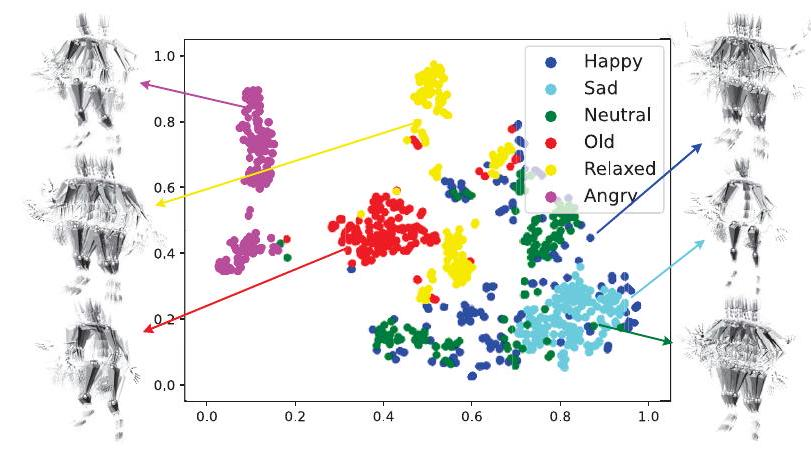
\includegraphics[width=0.7\linewidth]{images/emotion_dataset.jpg}
    \caption[Biểu đồ tSNE với các phong cách khác nhau]{Hiển thị tSNE của các cử chỉ với các phong cách khác nhau và bản đồ bóng của cử chỉ xương cơ với phong cách tương ứng. Ví dụ, với cử chỉ 'Old', hông và đầu gối của nó uốn cong hơn, và tay của nó cơ bản nằm ở đầu gối hoặc hông.}
    \label{fig:emotiondataset}
\end{figure}

Chúng tôi cũng vẽ biểu đồ xương cơ được tạo ra bởi phong cách tương ứng trong hình, và có thể thấy rằng đối với phong cách 'Old', hông và đầu gối của nó uốn cong hơn, và tay của nó cơ bản nằm ở đầu gối hoặc hông; với phong cách 'Sad', đầu của nó đang nghiêng và tay nó ở một vị trí thấp hơn; với phong cách 'Relax', hông của nó đang chuyển lên phía trước và tư thế đứng của nó là thoải mái; với phong cách 'Angry', tay của nó di chuyển lên và xuống nhanh chóng. Lưu ý rằng mặc dù sự khác biệt giữa cử chỉ phong cách 'trung tính' và 'Happy' vẫn khá rõ ràng trong việc thị giác hóa phong cách của xương cơ, tức là với phong cách 'Happy', vị trí tay của nó là cao hơn và biên độ của nó lớn hơn, tuy nhiên tSNE của chúng gần như kết hợp với nhau. Trong phân tích của chúng tôi, điều này xảy ra vì bài nói trung tính gọi là vẫn chứa thông tin như cảm xúc và ngữ nghĩa mà có trong các đặc trưng WavLM. Sự cân bằng giữa phong cách từ âm thanh $a$ và từ phong cách $s$ có thể được kiểm soát thêm bằng cách chỉnh sửa cường độ phong cách $\gamma$.

\subsection{Khả năng chỉnh sửa Phong cách của cử chỉ}

Để phân tích sâu hơn mối quan hệ giữa cường độ phong cách và phong cách được ngụ ý bởi bài nói, chúng tôi chọn phong cách 'Happy' và phong cách 'Old' và đặt $\gamma=1$ và 3 trong \autoref{eq:denoise}. Ngoài ra, để so sánh kết quả, chúng tôi đặt $\gamma=0.5$ trong \autoref{eq:denoise}, để nội suy giữa các phong cách khác nhau. Các tham số khác không thay đổi, và chúng tôi vẽ kết quả tạo ra cử chỉ trong 12 giây, với FPS $=1$ như thể hiện trong \autoref{fig:stylesample}.


Như thấy trong \autoref{fig:stylesample}, chúng ta có thể thấy rằng khi chúng ta sử dụng phong cách 'Happy' với $\gamma=3$, cả quá trình xoay cơ thể và chuyển động tay đều lớn nhất, và vị trí tay của nó là cao nhất; ngược lại, khi chúng ta sử dụng phong cách 'Old' với $\gamma=3$, hông của nó uốn cong nhất, tay hầu như không được nâng lên, và không có nhiều sự thay đổi trong toàn bộ chuỗi chuyển động; còn đối với ba kết quả khác, cường độ phong cách của chúng ở giữa hai trường hợp trên, và phong cách dần thay đổi từ vui vẻ đến già từ trên xuống dưới. Do kiến trúc mô hình của chúng tôi, cử chỉ và bài nói được tạo ra phù hợp hơn, mặc dù các phong cách này không giống nhau. Lưu ý rằng khi chúng ta sử dụng phong cách 'Happy' và 'Old' với $\gamma=0.5$, kết quả gần với việc sử dụng phong cách 'Happy' với $\gamma=1$, trong khi phong cách 'Old' gần như không thể cảm nhận được. Quan sát này tiếp tục xác nhận phát hiện trước đó rằng phong cách 'Happy' được nhúng trong bài nói 'trung tính' được sử dụng để kiểm thử. Phát hiện này hữu ích, ví dụ, chúng tôi đã phát hiện trong các thử nghiệm của mình rằng nếu chúng ta muốn kiểm soát bài nói 'Happy' để tạo ra cử chỉ 'buồn', $\gamma=1$ cơ bản là không hiệu quả vì mô hình có thể học được phong cách vui vẻ từ bài nói. Vì có sự liên kết giữa phong cách của bài nói và phong cách của cử chỉ, việc đặt $\gamma$ lớn hơn có thể chỉnh sửa phong cách tốt hơn. Do đó, chúng ta có thể tạo ra các cử chỉ không tồn tại trong tập dữ liệu gốc (ví dụ, cử chỉ cho bài nói 'Happy' nhưng có phong cách 'buồn') thông qua cường độ phong cách.


% Nghiên cứu Người dùng. 
Hơn nữa, chúng tôi muốn khám phá mối quan hệ giữa cường độ phong cách và độ giống con người cũng như sự phù hợp với ngôn ngữ, nên chúng tôi đã tiến hành một nghiên cứu người dùng. Để tránh phong cách trong ngôn ngữ nói ảnh hưởng đến việc đánh giá của người tham gia, giống như trước đó, chúng tôi chỉ kiểm soát cường độ của các phong cách cho một bài nói trung tính và sau đó yêu cầu người tham gia đánh giá ba chiều đặc trưng trước đó. ExampleGesture \cite{ghorbani2023zeroeggs} cũng có thể kiểm soát việc tạo ra các phong cách khác nhau của các cử chỉ từ cùng một bài nói. Vì vậy, chúng tôi chọn nó làm mô hình tham chiếu. Vì các cử chỉ được tạo ra ở đây không tồn tại trong tập dữ liệu, bài nói trung tính với phong cách trung tính được sử dụng làm tham chiếu. Kết quả được thể hiện trong \autoref{fig:mosscore}.


%\begin{figure}
%    \centering
%    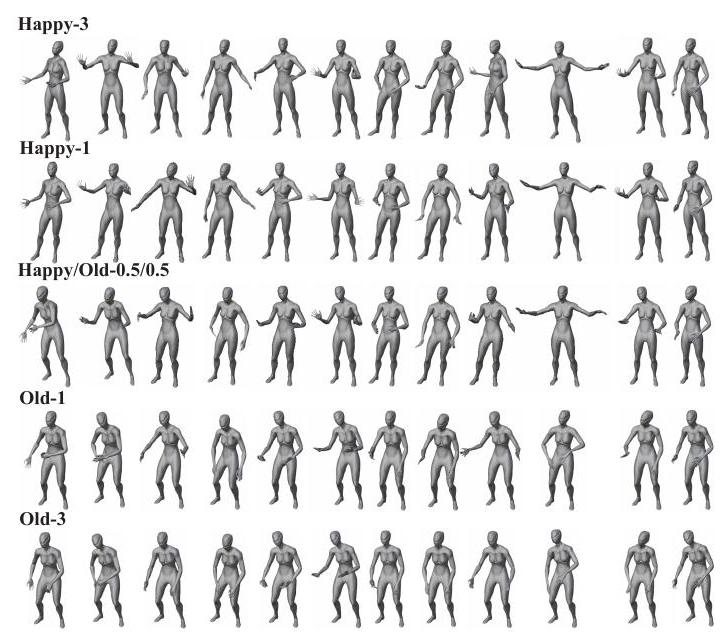
\includegraphics[width=\linewidth]{images/style_sample.jpg}
%    \caption[Chỉnh sửa phong cách và nội suy]{Chỉnh sửa phong cách và nội suy. Từ trên xuống dưới, cơ thể xoắn và chuyển động tay dần giảm và vị trí tay trở nên thấp hơn. Mặc dù có sự thay đổi về phong cách, các cử chỉ được tạo ra vẫn khớp tốt với bài nói trong các phong cách khác nhau}
%    \label{fig:stylesample}
%\end{figure}


% % Hình 6: 

\begin{figure}
    \centering
    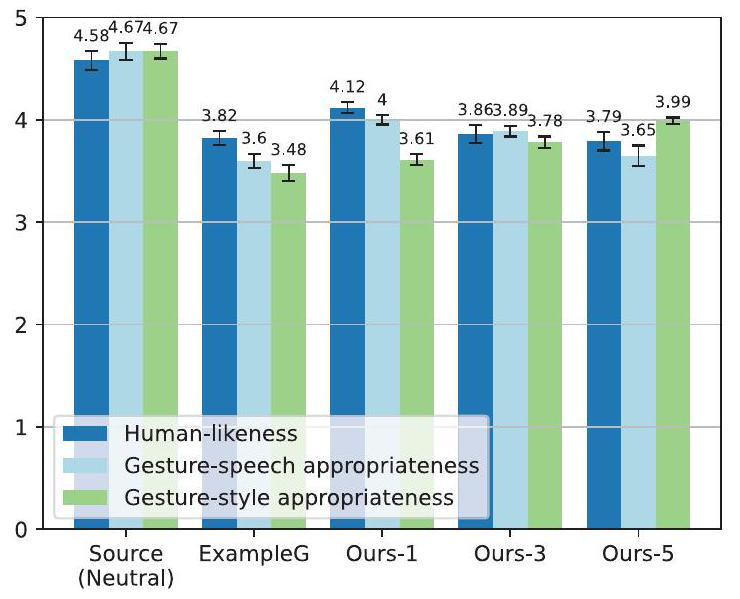
\includegraphics[width=\linewidth]{images/mos_score.jpg}
    \caption[Kết quả trung bình của MOS]{Kết quả trung bình của MOS với khoảng tin cậy $95\%$ cho ba chiều. 'Ours-$\gamma$' chỉ ra cường độ kiểm soát phong cách $\gamma$ của mô hình của chúng tôi. Mô hình của chúng tôi vượt trội đáng kể so với ExampleGesture tổng thể và có thể chỉnh sửa cường độ của các phong cách. Tham số $\gamma$ tăng và hai điểm số còn lại sẽ giảm một cách hợp lý.}
    \label{fig:mosscore}
\end{figure}


Kết quả cho thấy rằng mô hình của chúng tôi tương tự như ExampleGesture về mặt phù hợp giữa phong cách cử chỉ của kết quả ở $\gamma=1$, và độ giống con người cũng như sự phù hợp với ngôn ngữ của chúng tôi vượt quá ExampleGesture. Trong khi đó, phong cách trở nên đáng kể hợp lý hơn khi $\gamma$ tăng, nhưng điểm của hai chiều khác giảm. Điều này cũng là hiển nhiên, tức là nếu cường độ của phong cách 'Old' quá cao, tay ít được nâng lên và toàn bộ chuỗi chuyển động có biên độ nhỏ, vì vậy nó trông ít giống con người hơn và ít phù hợp với ngôn ngữ nói. Chúng tôi cũng thấy rằng kết quả của việc tạo ra kiểm soát phong cách (\autoref{fig:mosscore}) đã giảm so với kết quả của việc trực tiếp tạo ra phong cách tương ứng với ngôn ngữ nói (\autoref{fig:mosscore}). Chúng tôi tin rằng việc kiểm soát một phong cách nói để tạo ra một phong cách của cử chỉ khác là một nhiệm vụ "khó khăn và xung đột" bởi vì phong cách nói và phong cách của cử chỉ vẫn liên quan và kết hợp với nhau.

% \subsection{Khả năng tạo ra các cử chỉ đa dạng}

% \begin{figure}
%     \centering
%     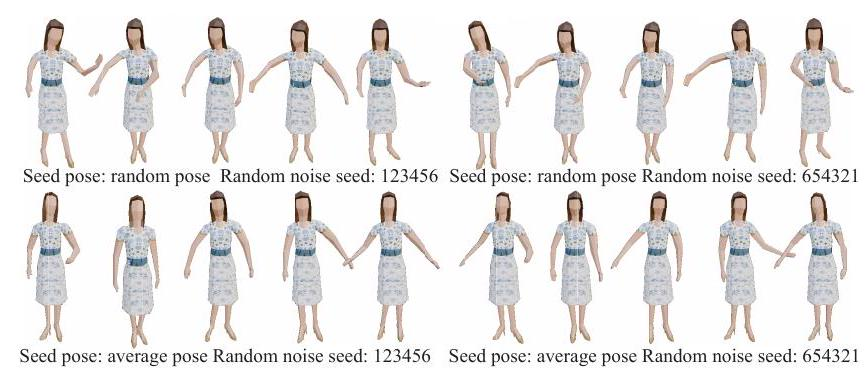
\includegraphics[width=\linewidth]{images/random_gesture_result.jpg}
%     \caption[Sự đa dạng của các cử chỉ]{Sự đa dạng của các cử chỉ. Mọi người thực hiện các cử chỉ đồng thoại khác nhau ở những thời điểm khác nhau trong các trạng thái khác nhau. Giống như con người thực tế, đối với cùng một bài nói, phương pháp của chúng tôi có khả năng tạo ra các cử chỉ khác nhau với hạt gieo khác nhau hoặc với cử chỉ nhiễu khác nhau}
%     \label{fig:randomgestureresult}
% \end{figure}


% \begin{center}
% \begin{tabular}{lcc}
% \hline
% \multicolumn{1}{c}{Tên} & \begin{tabular}{c}
% Con người $_{\text {tương đồng }} \uparrow$ \
% giống \
% \end{tabular} & \begin{tabular}{c}
% Phù hợp \
% ngôn ngữ - cử chỉ \
% \end{tabular} \
% \hline
% Sự thật & $4.15 \pm 0.11$ & $4.25 \pm 0.09$ \
% Chúng tôi & $\mathbf{4 . 1 1} \pm \mathbf{0 . 0 8}$ & $\mathbf{4 . 1 1} \pm \mathbf{0 . 1 0}$ \

% WavLM & $4.05 \pm 0.10$ & $3.91 \pm 0.11$ \
% tập trung chéo cục bộ & $3.76 \pm 0.09$ & $3.51 \pm 0.15$ \
% tập trung tự & $3.55 \pm 0.13$ & $3.08 \pm 0.10$ \
% chú ý + GRU & $3.10 \pm 0.11$ & $2.98 \pm 0.14$ \
% tập trung xuôi & $3.75 \pm 0.15$ & $3.23 \pm 0.24$ \
% \hline
% \end{tabular}
% \end{center}


% % Bảng 1: Kết quả nghiên cứu rút gọn. '-' chỉ ra các mô-đun không được sử dụng và ' + ' chỉ ra các mô-đun bổ sung. Chữ đậm chỉ ra số liệu tốt nhất.

% Do kiến trúc mô hình của chúng tôi, thậm chí đối với cùng một bài nói và phong cách, các cử chỉ nhiễu khác nhau và các hạt gieo khác nhau có thể tạo ra kết quả khác nhau, như thể hiện trong \autoref{fig:randomgestureresult}. Điều này giống như bài nói thực của con người, tạo ra các cử chỉ đồng thoại đa dạng liên quan đến vị trí ban đầu. Phân tích của chúng tôi trước đó được thực hiện trên chiều phong cách. Lưu ý rằng mô hình cũng thêm một mặt nạ ngẫu nhiên vào xử lý của hạt gieo, vì vậy nó cũng có thể nội suy và mở rộng các hạt gieo khác nhau để kiểm soát việc tạo ra cử chỉ với vị trí ban đầu khác nhau và đa dạng.

% \begin{table}[h]
% \caption{Đánh giá độ tương đồng và phù hợp ngôn ngữ-cử chỉ của các mô hình}
% \label{tab:evaluation}
% \begin{tabularx}{\textwidth}{l*{2}{>{\centering\arraybackslash}X}}
% \toprule
% \textbf{Tên} & \textbf{Con người (Tương đồng)} & \textbf{Phù hợp ngôn ngữ-cử chỉ} \\
% \midrule
% Sự thật & $4.15 \pm 0.11$ & $4.25 \pm 0.09$ \\
% Chúng tôi & $\mathbf{4.11 \pm 0.08}$ & $\mathbf{4.11 \pm 0.10}$ \\
% WavLM & $4.05 \pm 0.10$ & $3.91 \pm 0.11$ \\
% Tập trung chéo cục bộ & $3.76 \pm 0.09$ & $3.51 \pm 0.15$ \\
% Tập trung tự & $3.55 \pm 0.13$ & $3.08 \pm 0.10$ \\
% Chú ý + GRU & $3.10 \pm 0.11$ & $2.98 \pm 0.14$ \\
% Tập trung xuôi & $3.75 \pm 0.15$ & $3.23 \pm 0.24$ \\
% \bottomrule
% \end{tabularx}
% \end{table}

% \caption{Kết quả nghiên cứu rút gọn. '-' chỉ ra các mô-đun không được sử dụng và ' + ' chỉ ra các mô-đun bổ sung. Chữ đậm chỉ ra số liệu tốt nhất.}

% \section{Các thông tin thực nghiệm bổ sung}

% Hơn nữa, chúng tôi thực hiện nghiên cứu giảm thiểu để đánh giá ảnh hưởng hiệu suất của các thành phần khác nhau trong mô hình của chúng tôi. Vì phù hợp giữa cử chỉ và phong cách có thể được kiểm soát bằng tham số và ảnh hưởng đến hai chiều còn lại, chúng tôi đặt $\gamma$ là 1 và chỉ đánh giá sự giống nhân văn và phù hợp giọng nói để dễ so sánh. Kết quả của nghiên cứu giảm thiểu của chúng tôi được tóm tắt trong Bảng 1. Các so sánh hình ảnh của nghiên cứu này cũng có thể được tham khảo trong video bổ sung. Chúng tôi khám phá độ hiệu quả của các thành phần sau đây:
% (1) features WavLM 
% (2) local attention
% (3) local attention pattern
% (4) self-attention
% (5) attention
% Chúng tôi tiến hành thực nghiệm trên từng thành phần trong năm thành phần này, mỗi thành phần một lần.

% \subsection{Nghiên Cứu Người Dùng}
% Được hỗ trợ bởi kết quả trong Bảng 1, khi chúng tôi không sử dụng đặc trưng WavLM mà thay vào đó sử dụng 13 hệ số đầu tiên của hệ số cepstral tần số Mel (MFCC), điểm số của cả hai chiều đều giảm, đặc biệt là phù hợp giọng nói. Điều này là do các đặc trưng được trích xuất bởi mô hình WavLM đã được huấn luyện trước chứa nhiều thông tin như ngữ nghĩa và cảm xúc, giúp tạo ra các cử chỉ tương ứng. Khi không có sự chú ý cục bộ chéo, điểm số của cả hai chiều giảm rất nhiều. Bởi vì nhiều bước tạo ra cử chỉ chỉ liên quan đến các tương quan trong phạm vi ngắn, chú ý cục bộ có thể nắm bắt thông tin cục bộ tốt hơn, điều này khớp với quan sát của \cite{rae2020transformers}. Chỉ có chú ý tự dựa vào thông tin toàn cầu của các dãy dài trở nên ít hiệu quả hơn. 
% Cả giống nhân văn và sự phù hợp giữa cử chỉ và giọng nói giảm nhiều hơn khi chúng ta loại bỏ chú ý tự, ngụ ý rằng chú ý tự quan trọng hơn chú ý cục bộ vì có sự không đồng bộ tích cực giữa giọng nói và cử chỉ, và khó khăn để học đủ thông tin cử chỉ từ chỉ một cửa sổ cục bộ (gần như nửa giây) của giọng nói.
% Khi không sử dụng chú ý, chúng tôi thay thế nó bằng một mô hình dựa trên GRU, có kết quả tồi tệ nhất trong tất cả các mô hình, làm rõ thêm hiệu suất của cơ chế chú ý. 
% Ngoài ra, chúng tôi thực nghiệm sử dụng cấu trúc chú ý trong \autoref{fig:type_attention} và thấy rằng hiệu ứng trở nên tồi tệ hơn. Sự khác biệt duy nhất giữa việc thêm chú ý chuyển tiếp và chú ý cục bộ sử dụng trong mô hình của chúng tôi là cử chỉ được tạo ra với việc nhìn thêm vào thông tin giọng nói trong một cửa sổ tương lai. Điều này là một phát hiện thú vị, mặc dù có sự không đồng bộ ngầm giữa giọng nói và cử chỉ, theo một số cách, nó có thể chỉ ra rằng cử chỉ có liên quan hơn đến một khoảng thời gian ngắn trong hiện tại và quá khứ và không phải là một khoảng thời gian ngắn trong tương lai. Nó cũng có thể có khả năng rằng những người khác nhau có các phong cách khác nhau và tập dữ liệu này chỉ có một diễn viên cần được nghiên cứu thêm.

% % \section{Tập dữ liệu}

% % Bảng dữ liệu được chúng tôi trình bày dưới đây

% % \begin{adjustbox}{max width=\textwidth}
% % \begin{table}[htbp]
% %     \centering
% %     \begin{tabular}{|l|l|l|l|}
% %         \hline
% %         \textbf{Dataset} & \textbf{Modalities} & \textbf{Type} & \textbf{Download} \\
% %         \hline
% %         IEMOCAP & gesture_motion, audio, text, emotion & dialog & \href{https://sail.usc.edu/iemocap}{sail.usc.edu/iemocap} \\
% %         & & & \href{https://arxiv.org/pdf/1810.12541.pdf}{[paper]} \\
% %         \hline
% %         Creative-IT & gesture_motion, audio, text, emotion & dialog & \href{https://sail.usc.edu/CreativeIT/ImprovRelease.htm}{sail.usc.edu/CreativeIT} \\
% %         \hline
% %         Gesture-Speech Dataset & gesture_motion, audio & monolog & \href{https://www.dropbox.com/sh/j419kp4m8hkt9nd/AAC_pIcS1b_WFBqUp5ofBG1Ia?dl=0}{dropbox} \\
% %         \hline
% %         CMU Panoptic & gesture_motion, audio, text & dialog & \href{http://domedb.perception.cs.cmu.edu}{domedb.perception.cmu} \\
% %         & & & \href{https://arxiv.org/abs/1612.03153}{[paper]} \\
% %         \hline
% %         Speech-Gesture & gesture_motion, audio & monolog & \href{https://github.com/amirbar/speech2gesture}{amirbar/speech2gesture} \\
% %         & & & \href{https://arxiv.org/abs/1906.04160}{[paper]} \\
% %         \hline
% %         TED Dataset & gesture_motion, audio & monolog & \href{https://github.com/youngwoo-yoon/youtube-gesture-dataset}{youtube-gesture-dataset} \\
% %         & & & \href{https://sites.google.com/view/youngwoo-yoon/projects/co-speech-gesture-generation}{[homepage]} \\
% %         \hline
% %         Talking With Hands & gesture_motion, audio & dialog & \href{https://github.com/facebookresearch/TalkingWithHands32M}{facebookresearch/TalkingWithHands32M} \\
% %         & & & \href{https://personalrobotics.cs.washington.edu/publications/lee2019handmotiondataset.pdf}{[paper]} \\
% %         \hline
% %         PATS & gesture_motion, audio, text & monolog & \href{https://chahuja.com/pats}{chahuja.com/pats} \\
% %         & & & \href{https://arxiv.org/pdf/2007.12553v1.pdf}{[paper]} \\
% %         \hline
% %         Trinity Speech-Gesture I & gesture_motion, audio, text & monolog & \href{https://trinityspeechgesture.scss.tcd.ie/data/Trinity%20Speech-Gesture%20I/GENEA_Challenge_2020_data_release}{Trinity Speech-Gesture I} \\
% %         \hline
% %         Trinity Speech-Gesture II & gesture_motion, audio, segment & monolog & \href{https://trinityspeechgesture.scss.tcd.ie/data/Trinity%20Speech-Gesture%20II}{Trinity Speech-Gesture II} \\
% %         \hline
% %         Speech-Gesture 3D extension & gesture_motion, audio & monolog & \href{https://nextcloud.mpi-klsb.mpg.de/index.php/s/7LzxGSepzrndg2x}{nextcloud.mpi-klsb} \\
% %         \hline
% %         Talking With Hands GENEA Extension & gesture_motion, audio, text & dialog & \href{https://zenodo.org/record/6998231}{zenodo/6998231} \\
% %         & & & \href{https://dl.acm.org/doi/abs/10.1145/3536221.3558068}{[paper]} \\
% %         \hline
% %         SaGA & gesture_motion, audio, properties & dialog & \href{https://www.phonetik.uni-muenchen.de/Bas/BasSaGAeng.html}{phonetik.uni-muenchen} \\
% %         & & & \href{https://pub.uni-bielefeld.de/record/2001935}{[paper]} \\
% %         \hline
% %         SaGA++ & gesture_motion, audio, properties & dialog & \href{https://zenodo.org/record/6546229}{zenodo/6546229} \\
% %         \hline
% %         ZEGGS Dataset & gesture_motion, audio & monolog & \href{https://github.com/ubisoft/ubisoft-laforge-ZeroEGGS}{ubisoft-laforge-ZeroEGGS} \\
% %         & & & \href{https://arxiv.org/abs/2209.07556}{[paper]} \\
% %         \hline
% %         BEAT Dataset & gesture_motion, audio, text, properties, emotion & dialog, monolog & \href{https://pantomatrix.github.io/BEAT}{github.io/BEAT} \\
% %         & & & \href{https://arxiv.org/pdf/2203.05297.pdf}{[paper]} \\
% %         \hline
% %     \end{tabular}
% % \end{table}
% % \end{adjustbox}
% % % \caption{List of Datasets in Speech and Gesture Domain}
% % \label{tab:datasets}


% Kêt luận
\chapter{Kết luận}
\label{Chapter5}

Trong bài báo này, chúng tôi đề xuất \textbf{OHGesture}, một phương pháp dựa trên mô hình diffusion để tạo ra đồng thời cử chỉ dựa trên âm thanh. \textbf{OHGesture} thể hiện ba điểm mạnh chính:

1) Dựa trên một mô hình diffusion, ánh xạ xác suất tăng cường sự đa dạng trong khi cho phép tạo ra các cử chỉ chất lượng cao, giống con người.

2) Mô hình của chúng tôi tổng hợp các cử chỉ sao cho chúng khớp với nhịp âm thanh và ngữ nghĩa văn bản dựa trên các cơ chế tập trung chéo và tập trung tự.

3) Sử dụng phương pháp huấn luyện hướng dẫn không cần bộ phân loại, chúng ta có thể kiểm soát các điều kiện cụ thể, tức là phong cách và cử chỉ ban đầu, và thực hiện nội suy hoặc mở rộng để đạt được một mức kiểm soát cao đối với các cử chỉ được tạo ra.

Đánh giá chủ quan cho thấy rằng mô hình của chúng tôi vượt trội so với các phương pháp hiện có trong nhiệm vụ tạo ra cử chỉ đồng thời dựa trên âm thanh và thể hiện khả năng thao tác phong cách cao hơn. Còn nhiều không gian để cải thiện trong nghiên cứu này, ví dụ, giải quyết vấn đề nhiều bước lấy mẫu và tiêu thụ thời gian lâu của các phương pháp diffusion để sử dụng trong các hệ thống thời gian thực là hướng nghiên cứu của chúng tôi trong tương lai.

% Trong phần này chúng tôi đưa ra các kết quả đạt được của mô hình chúng tôi, chúng tôi cố gắng tìm hiểu các đặc trưng của các bộ dữ liệu tương ứng để cố gắng lý giải thích tại sao mô hình của chúng tôi hoặc các công trình khác có được kết quả tốt trên tập dữ liệu tương ứng đó. Những kết quả của hai đề xuất của chúng tôi cũng như các dịnh hướng nghiên cứu của chúng tôi trong tương lai.

% Mặc dù kết quả chúng tôi cho thấy phương pháp của chúng tôi có hiệu suất tương đương với các mô hình học sâu hiện đại (state-of-art) và có ưu thế vượt trội trong thời gian đào tạo khoảng 17 phút so với thời gian hàng giờ của phương pháp học sâu khác nhưng không phải là các mô hình học sâu này không đáng nghiên cứu. Chúng tôi cũng nhận thấy đối với những tập dữ liệu khó như FB15-237 hay WN18RR phương pháp của chúng tôi thường cho kết quả không tốt do các quan hệ tương tự hay nghịch đảo không không xuất hiện trong ví dụ đào tạo nên chúng tôi khó tạo ra các luật đủ tốt để có thể khái quát hóa trên toàn bộ đồ thị đẫn đến các kết quả không tốt. 
% Ngược lại đối với các phương pháp dựa trên học sâu lại có ưu thế rất lớn trong các tập dữ liệu này do có thể dễ dàng tính toán độ gần của các luật mới cần đánh giá so với các luật đã học từ đó có một kết quả khá tốt. Do đó chúng tôi cũng sẽ tiếp tục nghiên cứu các phương pháp học sâu và sẽ dùng phương pháp này làm đường cơ sở (base line) để so sánh với các nghiên cứu của chúng tôi trong tương lai. Một điểm yếu nữa của mô hình đựa trên luật của chúng tôi là mặc dù thời gian học là vượt trội nhưng thời gian để tính toán đưa ra đự đoán khá lâu do phải duyệt qua tất cả các luật được sinh ra mới có thể đưa ra dự đoán. Không giống như các phương pháp nhúng đồ thị khác thao tác này có thể dễ dàng tính toán.

% Đối với hai thuật toán mở rộng của chúng tôi trong việc thêm tri thức mới vào đồ thị chúng tôi nhận thấy rằng là vượt trội hoàn toàn so với các phương pháp học sâu. Ở các phương pháp học sâu điều này đường như chưa được ai chú trọng nghiên cứu mặc dù thời gian đào tạo một mô hình là tương đối mất thời gian. Khi có tri thức mới hầu hết các mô hình phải đào tạo lại toàn bộ điều này khá lãng phí. Chúng tôi cũng xem đây là mục tiêu tiếp theo cho chúng tôi khi nghiên cứu các mô hình học sâu trong tương lai. Gần đây nhánh học tăng cường (reinforcement learning) khá phát triển và nhóm tác giả Meilicke, Christian and Chekol \cite{meilicke2020reinforced} gần đây cũng đã có 1 nghiên cứu để tối ưu hóa lại phương pháp AnyBURL này. Chúng tôi cũng có ý định nghiên cứu về hướng này và cố gắng báo cáo lại trong một tương lai gần.


% Công trình của tác giả (nếu không có thì comment 02 dòng dưới)
% \addcontentsline{toc}{chapter}{Danh mục công trình của tác giả}
% \chapter*{Danh mục công trình của tác giả}
\label{Appendix1}

\begin{enumerate}
\item Tạp chí ABC
\item Tạp chí XYZ
\end{enumerate}

% In tài liệu tham khảo
\addcontentsline{toc}{chapter}{Tài liệu tham khảo}
\printbibheading[title={Tài liệu tham khảo}]

% \printbibliography[heading=subbibliography, title={Tiếng Việt}, keyword=Viet, resetnumbers=true]

% \DeclareNameAlias{sortname}{last-first}
% \DeclareNameAlias{default}{last-first}

\printbibliography[heading=subbibliography, title={Reference}, resetnumbers=1] 
% ===================================================================== %
% CHÚ Ý: phải gán lại resetnumbers=số tài liệu tham khảo tiếng Việt + 1 %
% ===================================================================== %

% Phần phụ lục
 \appendix
\section{BVH Data Processing Pipeline}
\label{appendix:BVHData}

\subsection{Skeleton Structure of a Character}
\label{appendix:BVHSkeleton}

Some skeleton joint names from the $75$ motion skeletons include:

{
	\small
	\texttt{Hips},
	\texttt{Spine},
	\texttt{Neck},
	\texttt{Head},
	\texttt{RightShoulder},
	\texttt{RightArm},
	\texttt{RightForeArm},
	\texttt{RightHand},
	\texttt{LeftShoulder},
	\texttt{LeftArm},
	\texttt{LeftForeArm},
	\texttt{LeftHand},
	\texttt{RightUpLeg},
	\texttt{RightLeg},
	\texttt{RightFoot},
	\texttt{RightToeBase},
	\texttt{LeftUpLeg},
	\texttt{LeftLeg},
	\texttt{LeftFoot},
	\texttt{LeftToeBase},
	...
}

\begin{figure}[h]
	\centering
	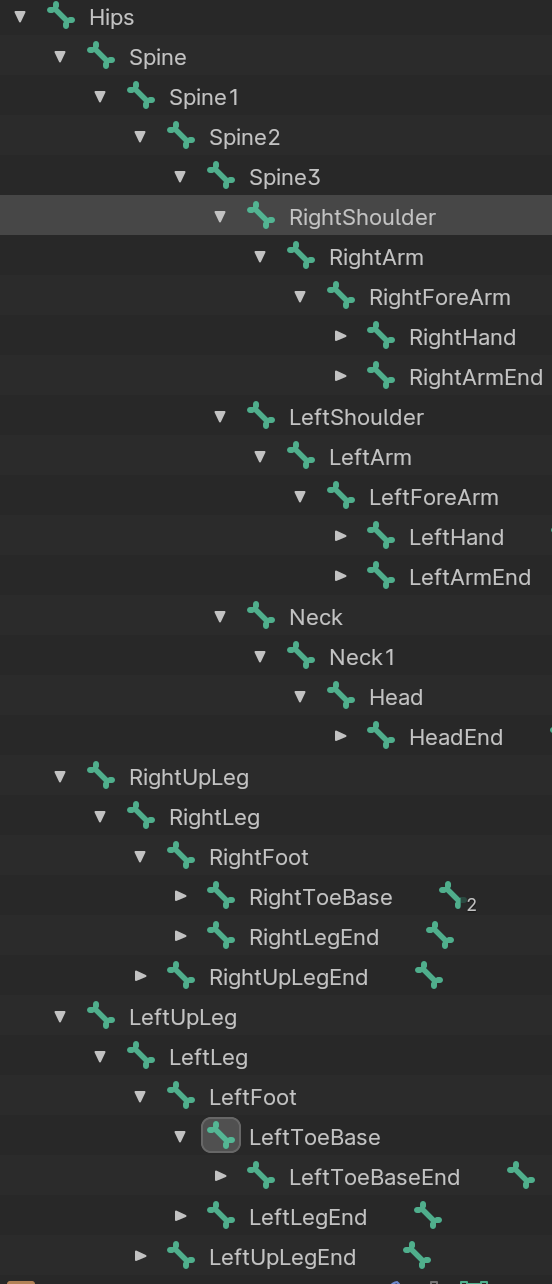
\includegraphics[height=10.5cm]{figures/Bone}
	\caption{Character skeleton}
	\label{fig:Bone}
\end{figure}

\subsection{Structure of a BVH File}
\label{appendix:BVHStructure}

A BVH (Biovision Hierarchy) file is a data format that contains information about the skeleton structure and motion data of bones in a skeletal system. A BVH file consists of two main parts: the skeleton hierarchy declaration and the bone motion data.

\begin{itemize}
	\item \textbf{HIERARCHY}:
	
	\begin{itemize}
		\item Defines the components and names of the skeleton joints, as well as the initial positions of the joints in the T-pose (motion capture actors extend their arms horizontally to form a "T").
		\item Defines the parent-child relationships from the root node to the leaf nodes of the skeleton, typically with the root node being the spine ($\texttt{Spine}$).
		\item Specifies the data to be recorded such as position or rotation angles along $X, Y, Z$ axes of each joint over time.
	\end{itemize}
	
	\item \textbf{MOTION}: A sequence of movements frame by frame, where each frame contains bone movement data as defined in the HIERARCHY section (e.g., rotation angles or positions).
\end{itemize}

\begin{figure}[htbp]
	\centering
	\begin{subfigure}{0.49\linewidth}
		\centering
		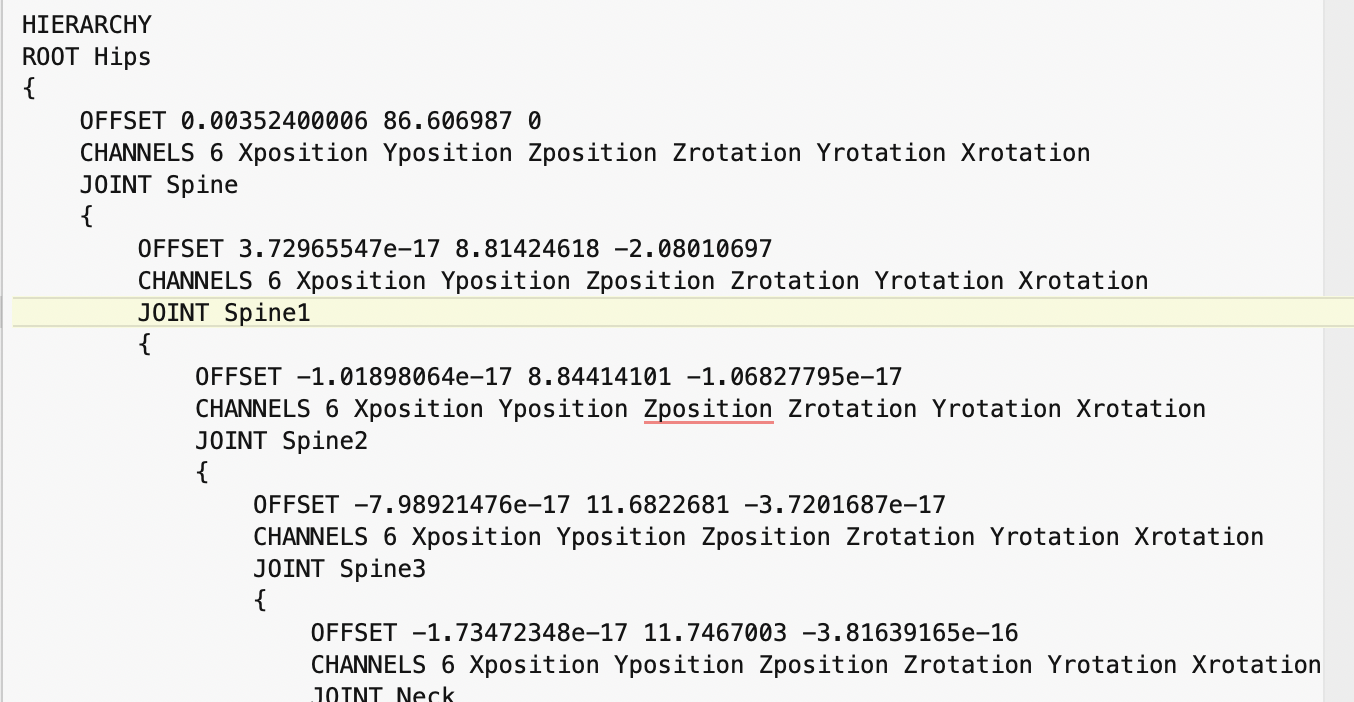
\includegraphics[width=\linewidth]{figures/BVH1}
		\caption{HIERARCHY in BVH file}
		\label{fig:BVH1}
	\end{subfigure}
	\hfill
	\begin{subfigure}{0.49\linewidth}
		\centering
		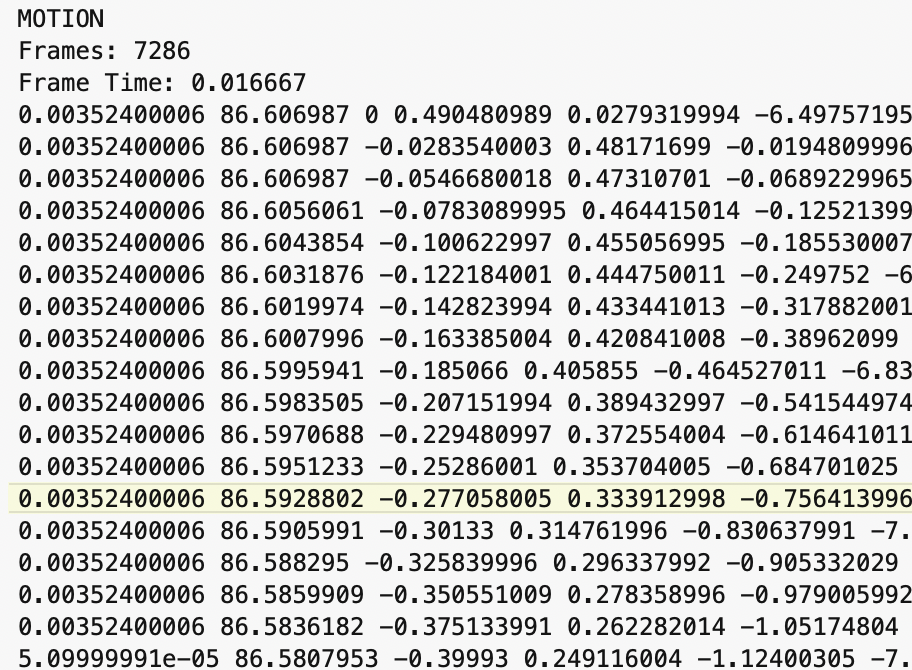
\includegraphics[width=\linewidth]{figures/BVH2}
		\caption{MOTION in BVH file}
		\label{fig:BVH2}
	\end{subfigure}
\end{figure}

$\mathbf{rotation}_i^{\operatorname{local}} = \{ \alpha ,\beta , \gamma \}$ represents the rotation angles around the $Z$, $Y$, and $X$ axes, respectively. The combined rotation in Euler space is:

\begin{equation}
	R = R_Z(\alpha) R_Y(\beta) R_X(\gamma)
\end{equation}

Where:

1. \textbf{Rotation matrix around axis \(Z\)}:

\[
R_Z(\alpha) = 
\begin{bmatrix}
	\cos(\alpha) & -\sin(\alpha) & 0 \\
	\sin(\alpha) & \cos(\alpha) & 0 \\
	0 & 0 & 1
\end{bmatrix}
\]

2. \textbf{Rotation matrix around axis \(Y\)}:

\[
R_Y(\beta) = 
\begin{bmatrix}
	\cos(\beta) & 0 & \sin(\beta) \\
	0 & 1 & 0 \\
	-\sin(\beta) & 0 & \cos(\beta)
\end{bmatrix}
\]

3. \textbf{Rotation matrix around axis \(X\)}:

\[
R_X(\gamma) = 
\begin{bmatrix}
	1 & 0 & 0 \\
	0 & \cos(\gamma) & -\sin(\gamma) \\
	0 & \sin(\gamma) & \cos(\gamma)
\end{bmatrix}
\]

To compute the motion coordinates of a character, the following operation is applied:

\begin{equation}
	\mathbf{position}_{\text{global}} = R \cdot \mathbf{position}_{\text{local}} + \mathbf{t}
\end{equation}


\subsection{Conversion from Euler Angles to Quaternions}
\label{appendix:BVHQuaternion}

To avoid Gimbal lock, Euler angle data must be converted into quaternion representation. Each bone's rotation from Euler angles in the ZYX order is represented as a quaternion $q = (q_w, q_x, q_y, q_z)$, with components calculated as follows:

First, compute the $\cos$ and $\sin$ values of half the rotation angles for each axis:

\begin{itemize}
	\item $c_{\alpha} = \cos\left(\frac{\alpha}{2}\right), \quad s_{\alpha} = \sin\left(\frac{\alpha}{2}\right)$
	\item $c_{\beta} = \cos\left(\frac{\beta}{2}\right), \quad s_{\beta} = \sin\left(\frac{\beta}{2}\right)$
	\item $c_{\gamma} = \cos\left(\frac{\gamma}{2}\right), \quad s_{\gamma} = \sin\left(\frac{\gamma}{2}\right)$
\end{itemize}

Based on the values above, the quaternion components are computed as:

\begin{itemize}
	\item $q_w = c_{\alpha} c_{\beta} c_{\gamma} + s_{\alpha} s_{\beta} s_{\gamma}$
	\item $q_x = c_{\alpha} c_{\beta} s_{\gamma} - s_{\alpha} s_{\beta} c_{\gamma}$
	\item $q_y = c_{\alpha} s_{\beta} c_{\gamma} + s_{\alpha} c_{\beta} s_{\gamma}$
	\item $q_z = s_{\alpha} c_{\beta} c_{\gamma} - c_{\alpha} s_{\beta} s_{\gamma}$
\end{itemize}

With the computed quaternion $q$, the global position of the bone $\mathbf{p}_{\text{global}}$ is determined by rotating the local position $\mathbf{p}_{\text{local}}$ using the formula:

\begin{equation}
	\mathbf{p}_{\text{global}} = q \cdot \mathbf{p}_{\text{local}} \cdot q^{-1} + \mathbf{t}
\end{equation}

where $\mathbf{t}$ is the origin position of the bone in global space.

 
\section{Sampling Process}

\begin{figure}[h]
	\centering
	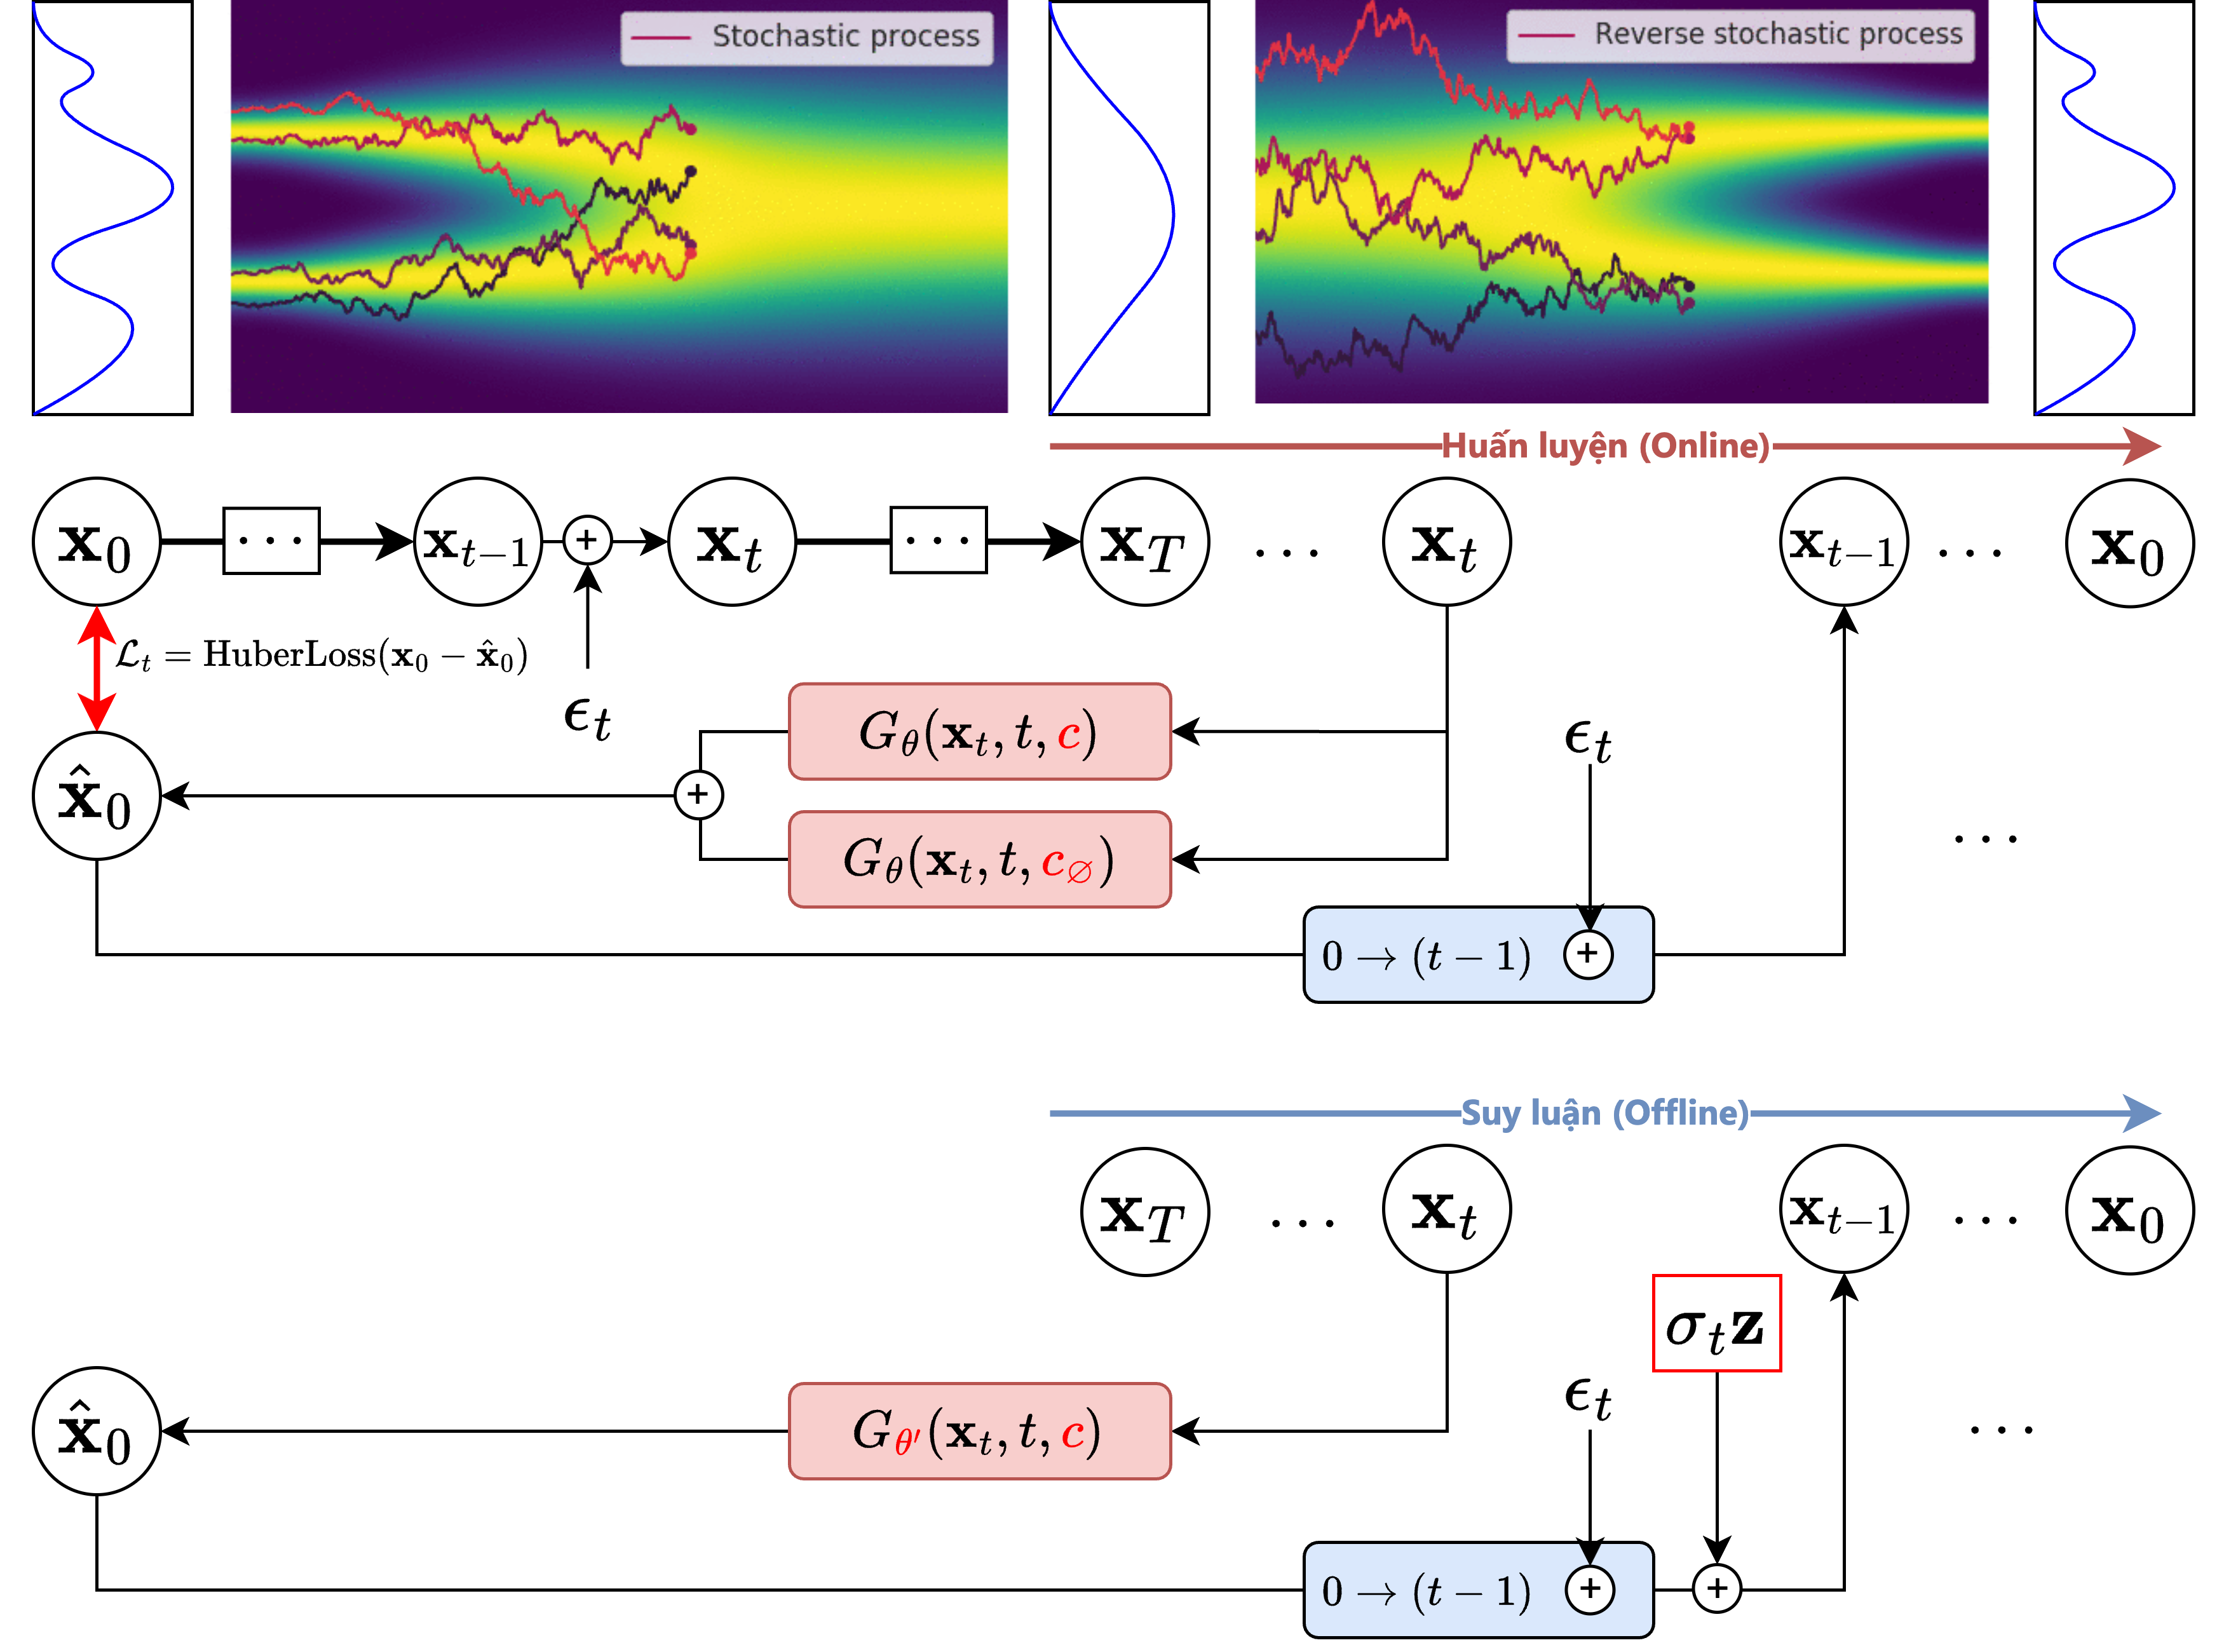
\includegraphics[width=0.8\linewidth]{figures/OnlineAndOffline}
	\caption{Offline (Training) and Online (Inference) Phases}
	\label{fig:OnlineAndOffline}
\end{figure}

\vspace{-5mm}

To generate gestures of arbitrary length, the original sequence is segmented into clips of length $M$.
During training, the seed gesture can be chosen by randomly selecting a gesture from the dataset or by averaging the clipped segments-here, the mean rotation angles are used.  
Generated frames are processed sequentially, with the last $N=8$ frames taken as the seed for the next iteration.  
For each clip, the gesture $\bx_{t}$ is denoised via $\hat{\bx}_{0} = G_{\theta'}(\bx_{t}, t, c)$; noise is re-added to obtain $\bx_{t-1}$, and the procedure repeats until $t=1$, yielding $\bx_{0}$.

\begin{algorithm}[h]
	\caption{Sampling in DeepGesture}
	\label{alg:sampling}
	\setlength{\baselineskip}{10pt}
	\begin{enumerate}
		\item Initialize with noise: $\mathbf{x}_T \sim \mathcal{N}(0, \mathbf{I})$.
		\item Retrieve $\sqrt{\alpha_t}$, $\sqrt{1 - \alpha_t}$, and $\sqrt{\bar{\alpha}_t}$ from training; precompute $\sigma_t$ from $\alpha_t$ for each timestep $t: 1 \rightarrow T$.
		\item Split each 4-second speech segment into $\mathbf{a} \in \mathbb{R}^{64000}$.  
		The initial seed gesture $\mathbf{s}$ is the data mean and later updated from the inferred gesture segment.  
		Select the desired emotion, obtain the transcript $\mathbf{v}$ from speech $\mathbf{a}$, and form the condition $c = [\mathbf{s}, \mathbf{e}, \mathbf{a}, \mathbf{v}]$.
		\item For each timestep, take $t$ \textbf{sequentially} from $[T, \dots, 1]$.
		\item Sample random noise $\mathbf{z} \sim \mathcal{N}(0, \mathbf{I})$.
		\item Infer $\hat{\mathbf{x}}_0^{(t)} = G_{\theta'}(\mathbf{x}_t, t, c)$.
		\item Diffuse $\hat{\mathbf{x}}_0^{(t)}$ from step $0 \rightarrow t$ to obtain $\hat{\mathbf{x}}_{t-1}^{(t)}$.
		\item Add noise: $\hat{\mathbf{x}}_{t-1} = \hat{\mathbf{x}}_{t-1}^{(t)} + \sigma_t \mathbf{z}$.
		\item Return to step 4.  
		When $t = 1$, output the denoised gesture $\hat{\mathbf{x}}_0$.
	\end{enumerate}
\end{algorithm}


\autoref{alg:sampling} starts by initializing the noisy gesture $\mathbf{x}_T$ from $\mathcal{N}(0, \mathbf{I})$.  
The values $\sqrt{\alpha_t}$, $\sqrt{1-\alpha_t}$, and $\sqrt{\bar{\alpha}_t}$ obtained during training, together with $\sigma_t$, are employed at each timestep (1 … $T$).  
Each 4-second speech segment is represented by $\mathbf{a}$, and the seed gesture $\mathbf{s}$ is taken as the data mean or from the previously inferred segment.  
The desired emotion and the transcript form the condition $c = [\mathbf{s}, \mathbf{e}, \mathbf{a}, \mathbf{v}]$.  
The algorithm proceeds sequentially from $T$ to 1: random noise $\mathbf{z}$ is generated, the model predicts $\hat{\mathbf{x}}_0^{(t)}$ from $\mathbf{x}_t$, $t$, and $c$, then $\hat{\mathbf{x}}_{t-1}^{(t)}$ is computed and perturbed with noise.  
This loop continues until $t=1$, after which the algorithm outputs the final denoised gesture $\hat{\mathbf{x}}_0$.


\end{document}

